\chapter{A unified model of the tension feasible set}
\label{chapter:3}

\usection{Introduction}
The force feasible set $\mathcal{F}$ can be modelized very differently depending on the context. Most representations are based either on an ellipsoid or a polytope (\cite{skuricOnLineFeasibleWrench2022}, \cite{rezzougUpperLimbIsometricForce2021b}, \cite{laisneGeneticAlgorithmsForce2023}, \cite{hernandezImprovingUpperlimbForce2017a}, \cite{bosscherWrenchfeasibleWorkspaceGeneration2006a}). Of strong interest is Chiacchio's force manipulability ellipsoid \cite{chiacchioForcePolytopeForce1997}. When a serial kinematic chain of $n$ degrees-of-freedom is considered, it is defined as $\mathcal{F}_{\text{Chiacchio}} := \{\mathbf{f}\in\mathbb{R}^3 \mid J^T\mathbf{f} = \tau,\quad \tau^T\tau\leq 1\}$
where $J^T$ is the transpose of the Jacobian matrix $J\in\mathbb{R}^{3\times n}$ expressed at the end-effector, and $\tau\in \IRn$ are the feasible torques. In Chiacchio's model, it is assumed that the torque feasible set is delimited by a sphere of radius $1$ ($\tau^T\tau \leq 1 \iff \|\tau \|_2 \leq 1$). In other words, the produced force ellipsoid described in the torque space corresponds geometrically to the central section of a unit $n$-dimensional sphere with $\im J^T$, the vector space spanned by the column of $J^T$. To express this intersected sphere in the Cartesian force space, it is sufficient to apply $(J^T)^+$, the Moon-Penrose pseudo-inverse of $J^T$ onto this set. Indeed, the pseudo-inverse acts as the classic inverse as long as the considered elements belong to $\im J^T$.

\begin{figure}[!htb]
    \captionsetup{justification=centering}
        \centering
        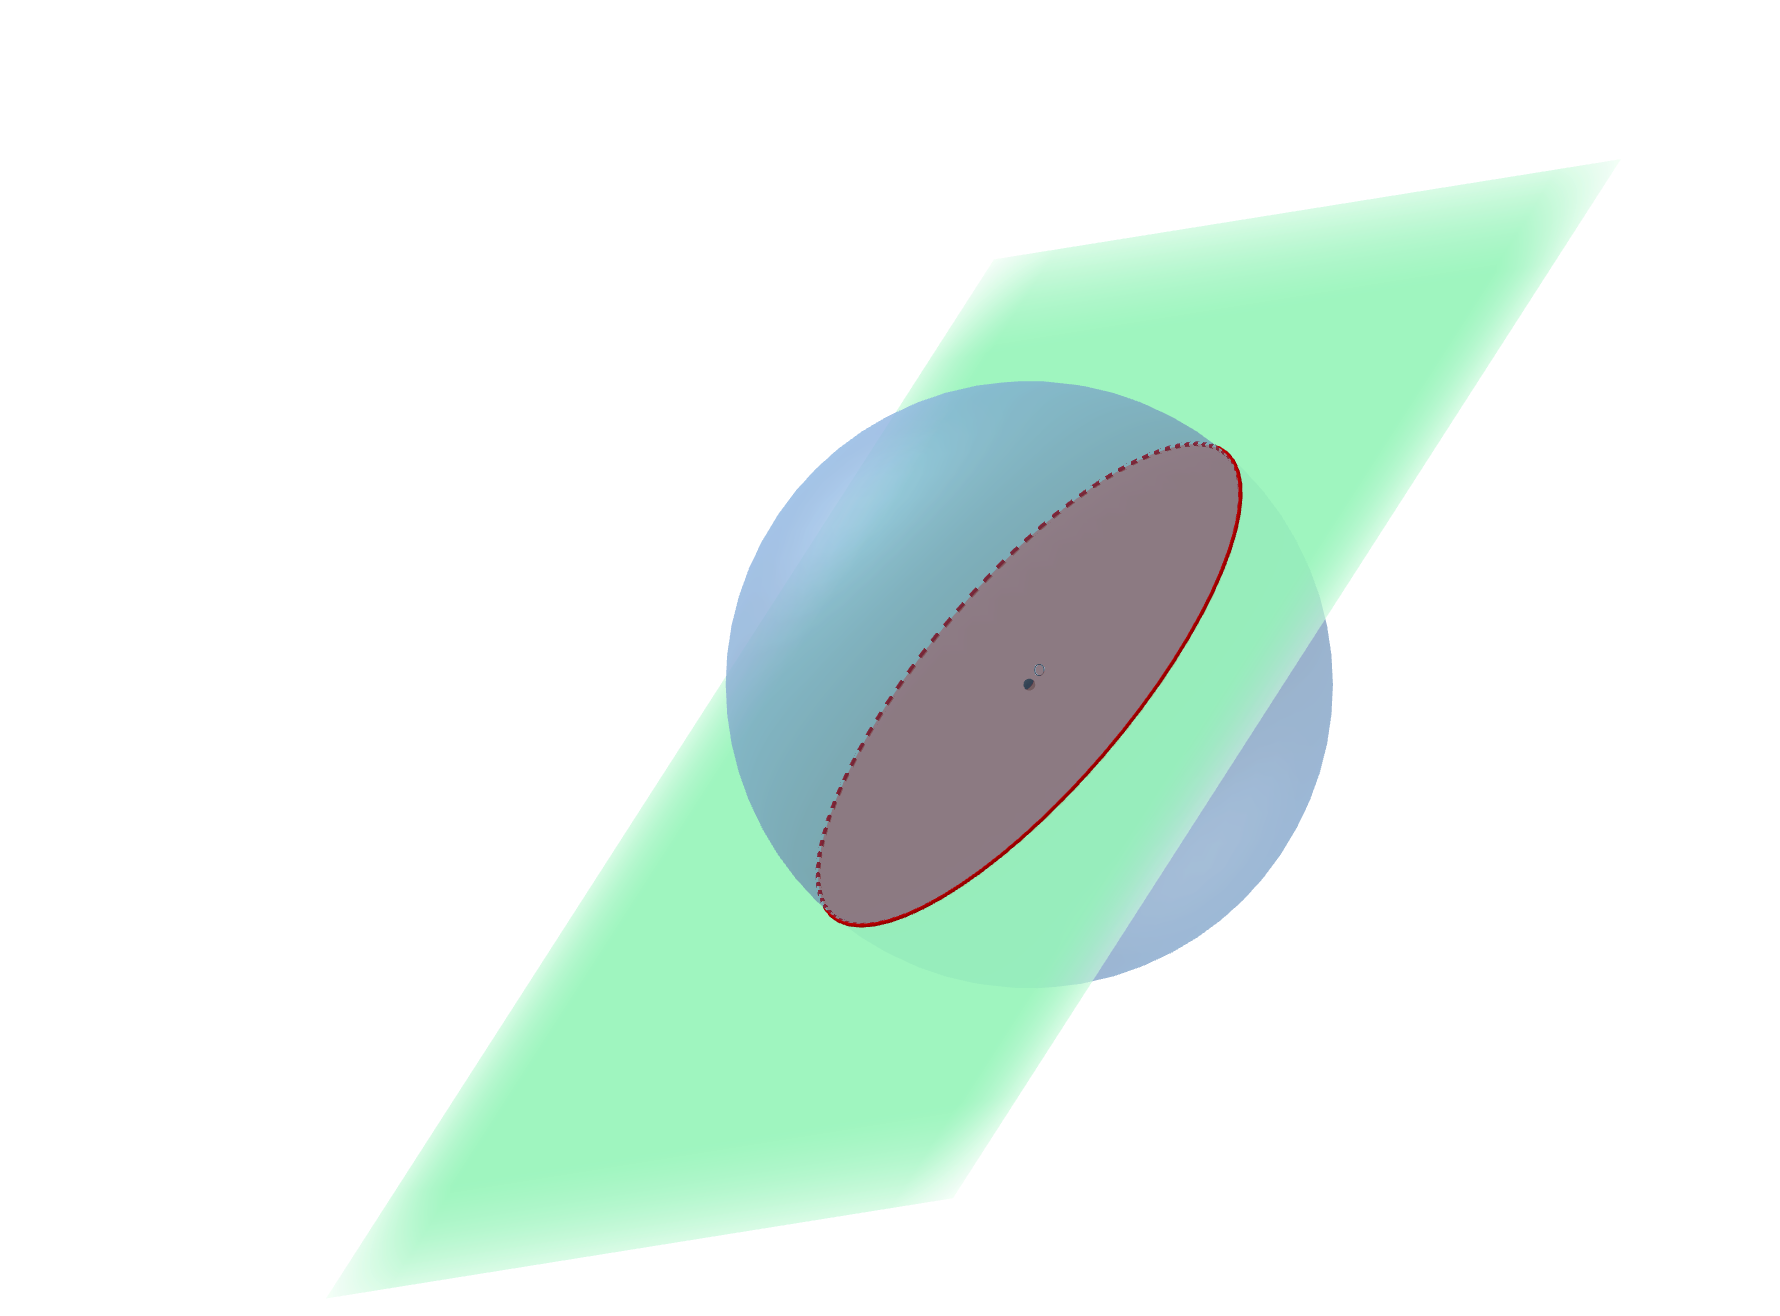
\includegraphics[trim={80 20 50 120}, clip, width=0.5\linewidth]{img/chapter_3/chiacchioellipsoid.png}
    \caption{Chiacchio's force ellipsoid expressed in the torque space (in red) \cite{chiacchioForcePolytopeForce1997}. The feasible torques (in blue) are modeled as a ball of radius 1. The intersection with $\im J^T$ (green plane) produces a lower-dimensional sphere (in red) defining Chiacchio's force ellipsoid in the torque space.}
    \label{fig:chiacchio_ellispoid}
\end{figure}

However, Chiacchio's construction lacks muscle considerations, which can be leveraged by adjusting the radius of the torque feasible sphere to ensure compatibility with experimental data \cite{rezzougUpperLimbIsometricForce2021b}. It may be relevant to ask ourselves if, contextually, this \emph{scaling} process sufficiently translates how muscles act on joint torques. Our approach is to consider \emph{all} possible models for the force feasible set and deduce general results which apply for any model choice. 

Let us consider the more general model of the static force feasible set. For $p \leq n \leq m$ integers, the force feasible set $\mathcal{F}$ of a $n$ degrees-of-freedoms of a $p$-dimensional kinematic chain equipped with $m$ muscles is defined for a specific posture as 
$$\mathcal{F} = \left\{ \mathbf{f}\in\IRp \mid J^T\mathbf{f} = -L^T\mathbf{t} - \mathbf{G},\quad \mathbf{t}\in\mathcal{T}\right\}$$
for $J^T\in\IRnp$ the transpose of the Jacobian matrix describing the mapping of end-effector forces onto the joint torques, $L\in\IRmn$ the lever-arm matrix such that $-L^T$ describes the mapping of the $m$ muscle tensions onto the joint torques, $\mathbf{G}\in\IRn$ the gravitational torque vector and $\mathcal{T}\subset \IRm$ the set of possible muscle tension combinations.

It is easily seen that Chiacchio's ellipsoid corresponds to the case in which: gravity is not considered; the tension set $\mathcal{T}$ is a centered sphere in $\IRm$ of radius 1; and $-L^T$ is an orthogonal projection from the tension space to the torque space. In other words, there are many assumptions on how muscles act onto joints. However, this general formulation has three major drawbacks: 1) the muscle geometry should be known in order to compute the lever arms in  $-L^T$; 2) the minimal and maximal tensions of each muscle should be known in order to estimate the possible values taken by $\mathbf{t}$ and finally, 3) the neuromuscular behavior should be understood to properly modelize the shape of $\mathcal{T}$. Indeed, the tension set can be also seen a linear transformation of the set of all possible muscle activations. Since muscles may be activated according to the activation of neighbour muscles (called muscular grouping), or activated according to a flexor-extensor relationship with another muscle, this is equivalent to assume a relation between muscles two-by-two. So the global shape of the tension set is determined by a linear transformation of the activation set. To summarize the construction:

\begin{figure}[!ht]
    \centering
    \captionsetup{justification=centering}
    \begin{tikzcd}
        \mathcal{F}' \subset \mathbb{R}^p & \mathcal{F} \subset \mathbb{R}^n \arrow[l] \arrow[l, "(J^T)^+"] & \mathcal{T}_o\subset \mathbb{R}^n \arrow[l, "\cap \im J^T"] & \mathcal{T}\subset \mathbb{R}^m \arrow[l, "-L^T - \mathbf{G}"]
    \end{tikzcd}
    \caption{Description of the geometric operations to derive the force feasible set in isometric conditions. The set of muscle tensions $\mathcal{T}$ is projected and translated onto the torque space to create the torque feasible set $\mathcal{T}_o$. It is then intersected with a vector space ($\im J^T$) to produce the force feasible set $\mathcal{F}$ described in the torque space, or conveniently in the Cartesian force space using $(J^T)^+$. In practice, we prefer to express $\mathcal{F}$ in the torque space since $(J^T)^+$ is a bijection between $\mathcal{F}$ and $\mathcal{F}'$.}
    \label{fig:formula_}
\end{figure}

A simple application of this general formula is when all muscles are considered to be all fully-activable at the same time. In other words, $\mathcal{T}$ is the transformation of a cube and we call it an \emph{orthotope}. In this case, $\mathcal{T}$ is projected onto the torque space to describe all feasible torques under the shape of a zonotope. The force feasible set is thus a polytope (intersection of a zonotope). With the orthotopic assumption over the tension set, we shall say that the force feasible set is modelized as a $\mathcal{T}_{\infty}$ model. If $\mathcal{T}$ is assumed to be a transformation of a sphere, then we call it a $\mathcal{T}_2$ model. A simple example is described in the figure \ref{fig:tension_models}.
\clearpage
\begin{minipage}{0.4\linewidth}
    \centering
    In a $\mathcal{T}_{\infty}$ model, $\mathcal{F}$ is a polytope.
\end{minipage}
\hfill
\begin{minipage}{0.4\linewidth}
    \centering
    In a $\mathcal{T}_2$ model, $\mathcal{F}$ is an ellipsoid.
\end{minipage}
\begin{figure}[!htb]
    \centering
    \captionsetup{justification=centering}
    \begin{minipage}{0.49\linewidth}
        \centering
        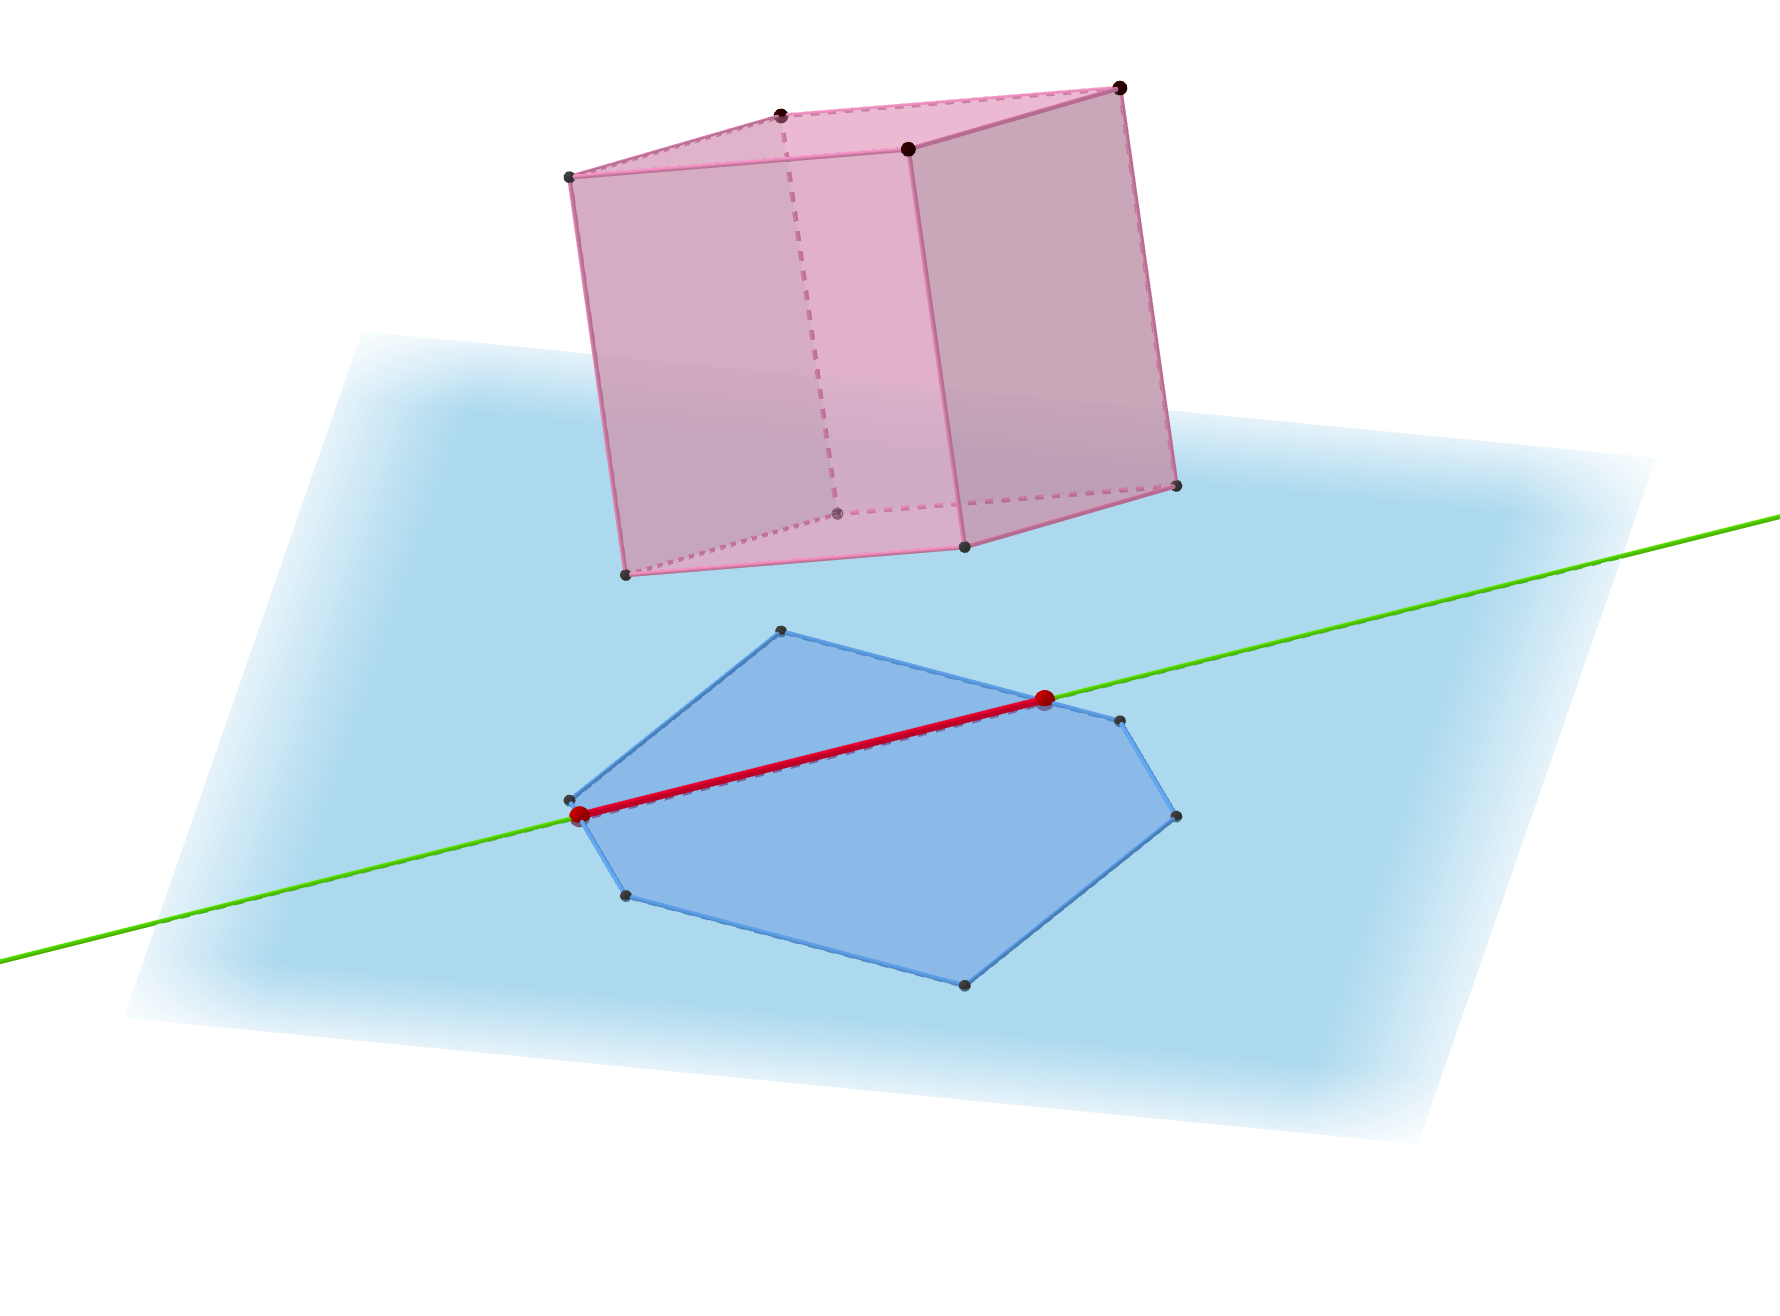
\includegraphics[trim={50 150 50 70}, clip, width=1\linewidth]{img/chapter_3/polytope_better_ggb.png}
    \end{minipage}
    \hfill
    \begin{minipage}{0.49\linewidth}
        \captionsetup{justification=centering}
        \centering
        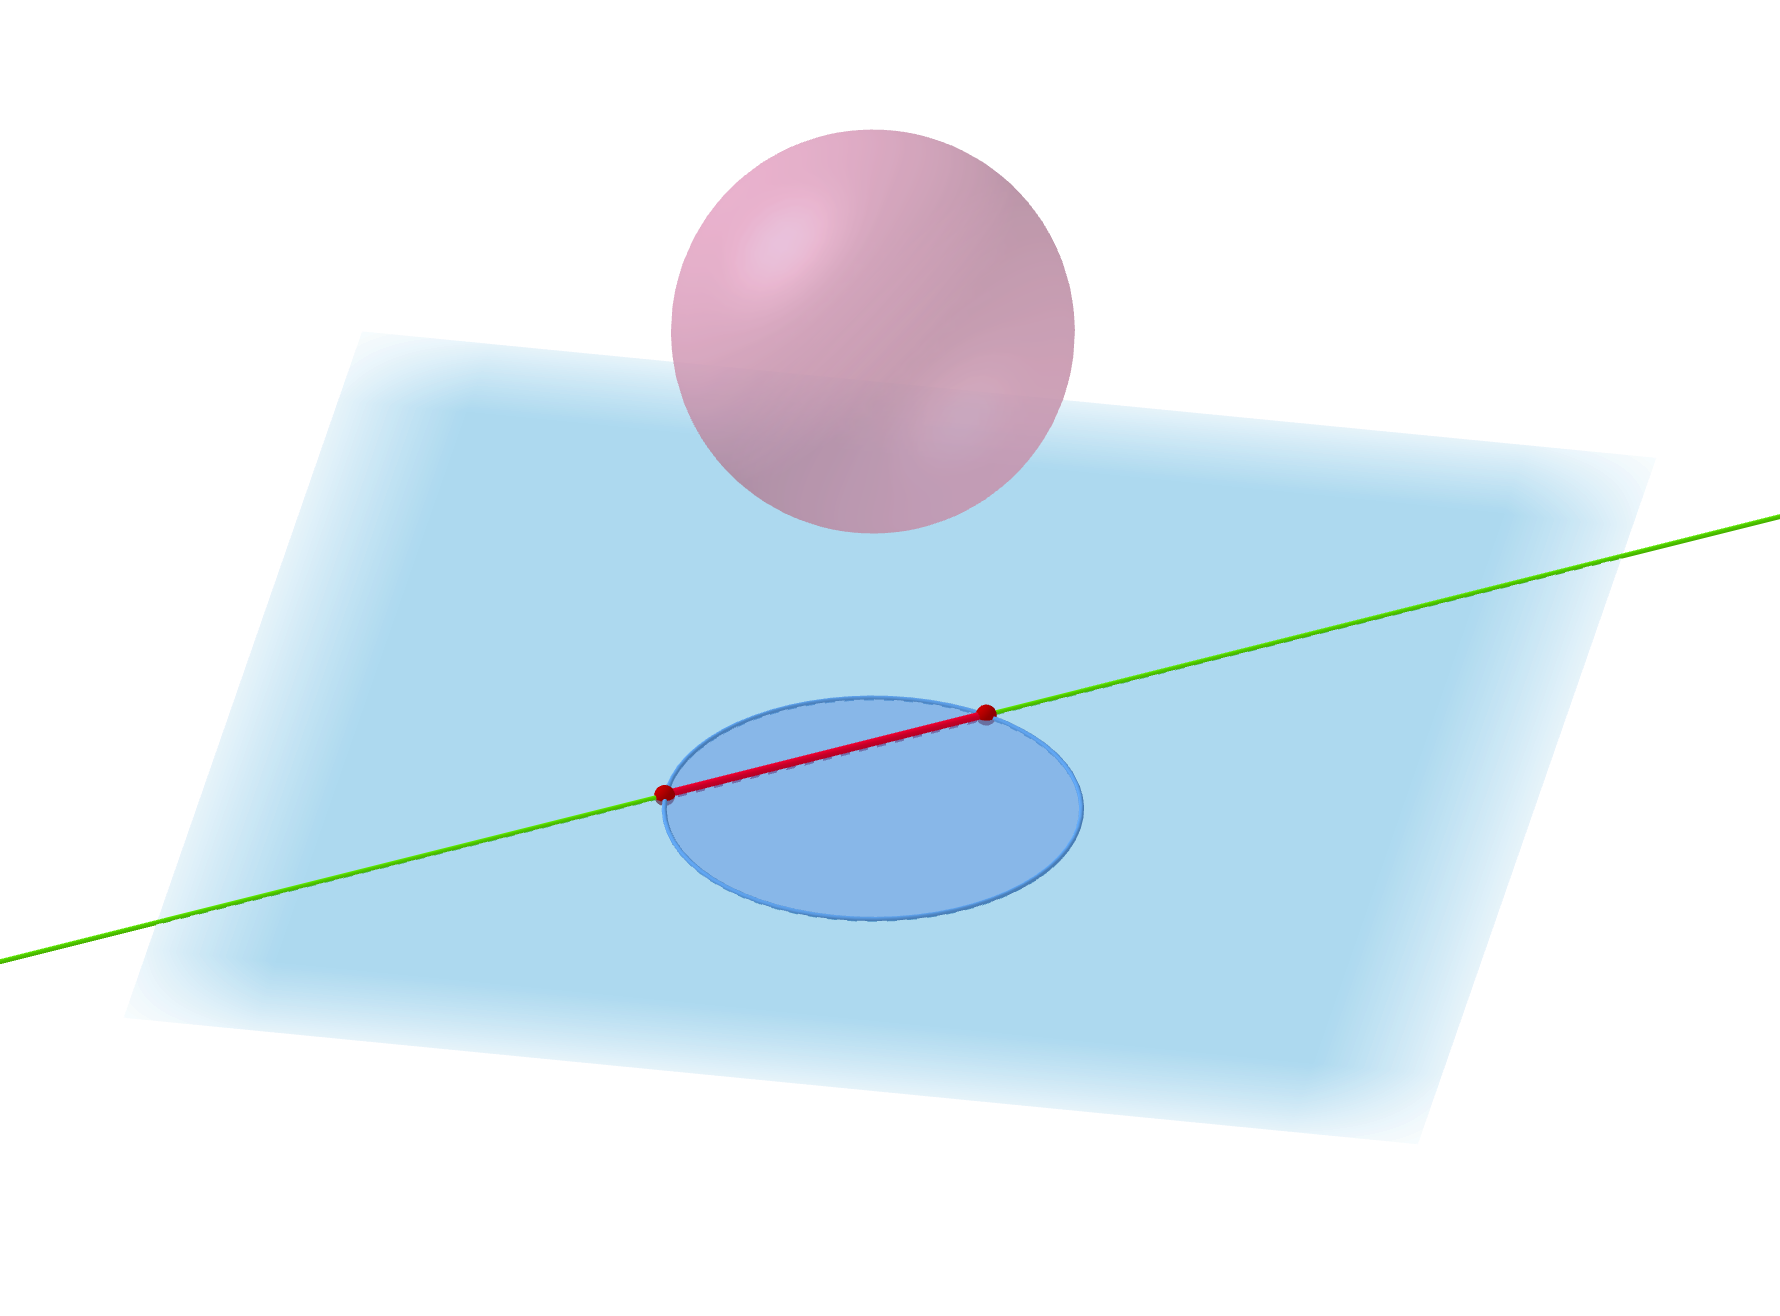
\includegraphics[trim={50 150 50 70}, clip, width=1\linewidth]{img/chapter_3/polytope_from_sphere_ggb.png}
    \end{minipage}
    \caption{Differences between the shape of the force feasible set $\mathcal{F}$ (in red) according to the modeling choice of the tension set $\mathcal{T}$ (in pink). A $\mathcal{T}_{\infty}$ model means that $\mathcal{T}$ is the transformation of a cube (\emph{i.e.} an orthotope), whereas a $\mathcal{T}_2$ model is the linear transformation of a sphere (\emph{i.e.} an ellipsoid). The force feasible set $\mathcal{F}$ can be constructed in two steps: first, $\mathcal{T}$ (in pink) is projected onto the torque space (light blue plane) and forms the torque feasible set $\mathcal{T}_o$ (in dark blue). Then, $\mathcal{T}_o$ is intersected by a subspace (green line). All elements in this intersection correspond to the force feasible set $\mathcal{F}$ described in the torque space.}
    \label{fig:tension_models}
\end{figure}

Unfortunately, it was suggested through experimental measurements of maximal force exertions at the hand that such a scaled Chiacchio's ellipsoid underestimates the measurements while the polytope overestimates them \cite{rezzougUpperLimbIsometricForce2021b}. These estimations were based on in silico force feasible sets, and required the scaling of a generic upper limb musculoskeletal model. 

\begin{figure}[!htb]
    \captionsetup{justification=centering}
        \centering
        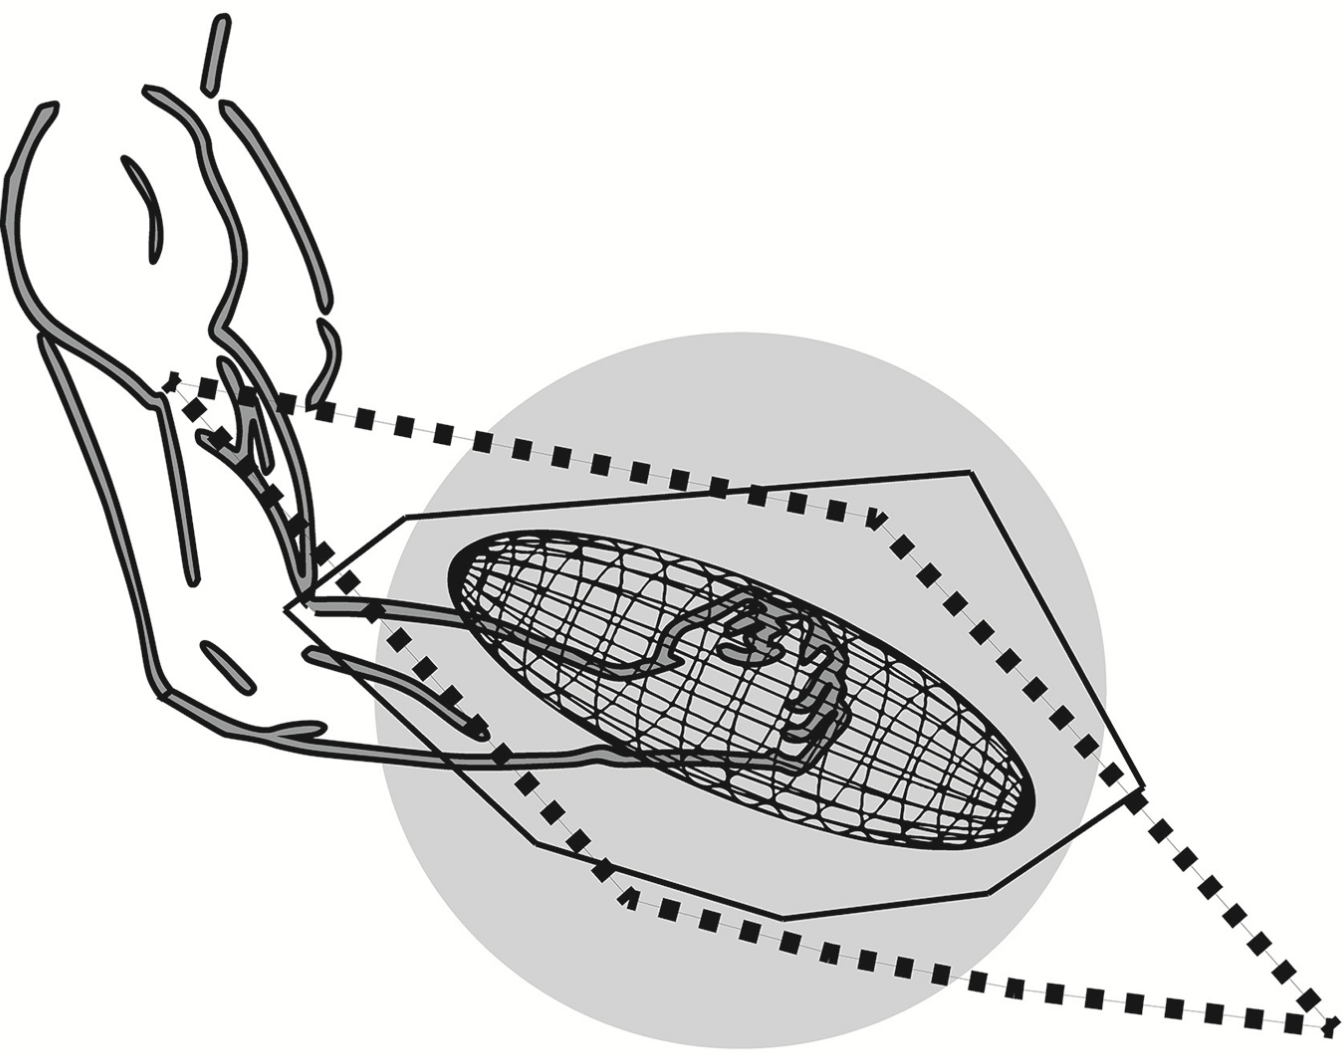
\includegraphics[trim={0 0 0 0}, clip, width=0.5\linewidth]{img/chapter_3/FFSComparisonRezzoug.png}
    \caption{Two modelized scaled force feasible set boundaries compared to experimental data; expressed in the sagittal plane relative to the upper-limb posture of one of the participant. The solid line corresponds to the convex hull of experimentally measured maximal force exertions. The black squares is the in silico force feasible set modelized as a polytope while the wire-frame is the ellipsoid version. The gray circle has a radius of 300N. Image extracted from Rezzoug et al. \cite{rezzougUpperLimbIsometricForce2021b}.}
    \label{fig:rezzoug_exp}
\end{figure}

Consequently, an ellipsoid or a polytope representation of the force feasible set do not seem to properly encapsulate measured experimental force exertions in size. They seem however to be close to global orientation of measured data. Since Chiacchio's ellipsoid does not require the knowledge of muscle lever arms, it may be assumed that it is $J^T$ which is at the core of this orientation property.

Now, in the above-mentionned $\mathcal{F}$ representations, they were chosen arbitrarily but they all have one common point: $\mathcal{T}$ is assumed to be convex and symmetric. A spherical shape is computationally practical, but does underestimate the expected size. A cubical shape leads to combinatorial issues to express the force feasible set, overestimates the expected size, and lead to unreasonnably sharp edges in the context of human. 

This chapter has three main objectives deriving from a deeper understanding of the mathematical formulation of the force feasible sets:
\begin{enumerate}[noitemsep]
    \item {Separate the notions of \emph{size} and \emph{shape} in $\mathcal{F}$ to better control them when fitting in silico force feasible sets to experimental data. It will be shown that $\mathcal{F}$ has an ellipsoidal shape for any modelization considered, and this approximation is better as the number of muscles considered increases. Also, $\mathcal{F}$'s size approximately depends on a coupling between the mean value of all maximal muscle tensions and the muscle path geometry;}
    \item {Compute how the muscle path geometry alone has an impact onto $\mathcal{F}$, and use it as an application to decide contextually whether are not if the personalization of muscle geometry of a scaled generic musculoskeletal model is a necessary process;}
    \item {Offer more perspectives on how should be modelized force feasible sets depending on context.}
\end{enumerate}

Also, we seek to find the most suitable force feasible set modelization such that their size and shape are coherent with experimental measurements in isometric conditions. Since these properties of depend on the how is modelized the tension set, our approach is to consider the class of all convex symmetric sets possible for $\mathcal{T}$. This is realized using the theory of Banach spaces, which is the focus of section \ref{sec:theory_banach_spaces}. This theory allows us to work in a more practical framework in which symmetric convex sets are considered as vector spaces equipped with different notion of size. 
Section \ref{sec:ellipsoidal_shape_ffs} dives into more depth called the Local Theory in order to show that whatever the choice of modeling of $\mathcal{T}$, there is a high probability of having a force feasible set resembling an ellipsoid. This probability is close to $1$ as the number of considered muscles increases, but the main result is that this is due to the geometric construction of the force feasible set. This section ends with a computable rewritting of the general description of the force feasible set directly in the tension space, so that it is easier to describe how muscle tension combinations contribute to the force feasible set.  However, this ellipsoidal approximation is a theoretical result, and computing it is surprisingly non-trivial and still depends on the model choice of $\mathcal{T}$. To overcome this difficulty, Section \ref{sec:projected_volume_problem} studies another branch of Banach theory, which we call \emph{the projection constant theory}. It is shown that the problem of fitting the size is directly related to the arbitrary modeling choice of the tension set $\mathcal{T}$ and propose an explicit computation for an adapted ellipsoid. Also, all previous sections served as getting familiar with theoretic tools to compare symmetric convex set, we shall apply this knowledge in section \ref{sec:sensitivity} to offer a novel index representing how the personalization of muscle paths geometry (locations of path points and via points) in a musculoskeletal model has an influence on the force feasible set. This index is independent of how $\mathcal{T}$ is modeled. This contextual index seeks to precise if the muscle geometries should be personalized in more details when scaling a generic musculoskeletal model to a subject.
This chapter concludes on summarizing this whole theoretical analysis of the force feasible set, and lead to the next two chapters derived as applications of the theory in a context of musculoskeletal model reconstruction.

\section{The theory of Banach spaces}
\label{sec:theory_banach_spaces}
This thesis considers a set-theoretic approach to modelize exertable forces by an individual. However, such an approach may not seem practical when comparing force feasible sets of two subjects, or understand how muscle tensions and muscle geometry influences the produced force sets. Since mathematics are, in a sense, the science of point of views, we shall consider a different perspective which still encapsulates our set vision. This section concentrates on describing the backbone of \emph{Banach spaces}, which is a structured manner to study the geometry of symmetric convex sets as well as describing how a unit metric transforms onto another.

\paragraph*{Banach space.} If $X$ is a \emph{complete normed vector space}, it is called a Banach space. \emph{Complete} means that every Cauchy sequence of $X$ converges towards a limit in $X$: in a sense, the space $X$ has no holes. It is also a \emph{normed} space, so the notion of \emph{size} exists for any element $x\in X$ and is called the \emph{norm of $x$}. It is denoted by $\|x\|_X$ and the subscript may be omitted when no confusion is possible. To be precise, $(X,\, \|\cdot \|_X)$ is a common notation for a Banach space. In this thesis, we concentrate on \emph{finite dimensional real-valued normed} vector spaces \emph{i.e.} the coefficients of a vector are real and there are a finite number of them. In this case, it is well-known that these kind of spaces are automatically complete, and thus Banach spaces.

In the following, we offer two approaches on the study of Banach spaces: the \emph{geometric} one, which may be the most intuitive and easiest to imagine, and the \emph{metric} perspective, in which a more physical meaning is emphasized:
\begin{enumerate}
    \item {\textbf{Geometrical perspective:} consider a Banach space to be a vector space with inside a symmetric convex set whose center of symmetry is the origin. This convex set can be a ball, an ellipsoid, a zonotope, a cube, etc as long as it is fully-dimensional and centrally symmetric. They are more commonly called \emph{unit balls}. As we would usually do in linear algebra by transforming a vector space onto another, here we should not forget to also \emph{deform} the convex set into another convex set;}
    \item {\textbf{Metric perspective:} a Banach space is essentially a vector space in which the physical notion of \emph{unit metric system} is properly defined. It is thus possible, to some extent, to study how a physical unit measure is transformed into another.}
\end{enumerate}

These two point of views allow us to make a parallel between the geometry components of the force feasible set and its more physical meaning. The choice of a perspective depends on the context: we shall show at some point that when considering a large number of muscles, force feasible sets resemble ellipsoids; but it is proven by showing that the Newton unit used to quantify muscle tension combinations transforms quadratically to become the Newton-meter unit of the torque space.

While a linear algebra background is assumed to be known from the reader, the geometric and metric perspective can be less familiar, especially when dimensions get large. We encourage the reader to adopt, for now, the geometric point of view to ensure a smooth reading. The next paragraphs lie common notions which are the basics of any study about Banach spaces.

\paragraph*{The $p$-norms and $\ell_p^n$ spaces.} Norms are tools for measuring the \emph{size} of $1$-dimensional elements (such as vectors). In $\IRn$, it is usual to consider the norm $\|\mathbf{x}\| = \sqrt{x_1^2 + \dots + x_n^2}$. It is called the \emph{euclidean} norm, or $2$-norm. When $\IRn$ is equipped with $\|\cdot \|_2$, we say that $\IRn$ is $n$-\emph{Euclidean}. However, this is not the only possible norm which can be equipped to $\IRn$. The $p$-norm $\|\cdot \|_p$ is defined as
$$\|\mathbf{x}\|_p = \left(\sum_{i=1}^n \vert x_i \vert^{p}\right)^{1/p}$$
and the euclidean norm corresponds to $\|\cdot\|_2$. It is also useful to define the $\infty$-norm:
$$\|\mathbf{x}\|_{\infty} = \lim_{p\to \infty} \|\mathbf{x}\|_p = \max_{i=1,\dots,n}\vert x_i\vert$$

$p$-norms encode \emph{analytically} the geometry of a specific type of centrally symmetric convex set. In other words, the surface of these sets is described as $\{\mathbf{x}\in \IRn \mid \|\mathbf{x}\|_p = 1\}$. Since we are interested in fitting shapes and understanding the possible shapes of the force and torque feasible sets, having an analytical tool to describe them is convenient.
To distinguish which $p$-norm is considered, we use the notation $\ell_p^n$ to represent the $n$-finite dimensional real vector space $\IRn$ equipped with the $p$-norm $\|\cdot \|_p$. 

\paragraph*{Unit balls.} A norm describes the size of a vector according to a reference value depending on its direction. Also, it depends on the dimension of the ambiant space. In other words, an \emph{arbitrary} choice of a norm onto a Banach space $X$ implies that we are defining how some directions in $X$ may influence the vector size. To consider all the possible influences (since there are infinitely many directions for $n\geq 2$), we can describe the set $\mathcal{B}_X = \{\mathbf{x}\in X \mid \|\mathbf{x}\|_X \leq 1 \}$, which is called the \emph{unit ball} of X. In the case of $\ell_p^n$ spaces, we denote $\mathcal{B}_p^n$ their unit $p$-ball, as shown in figure \ref{fig:pnorms} for $\ell_p^2$ spaces with various values of $p$.
\begin{figure}[!htb]
    \captionsetup{justification=centering}
        \centering
        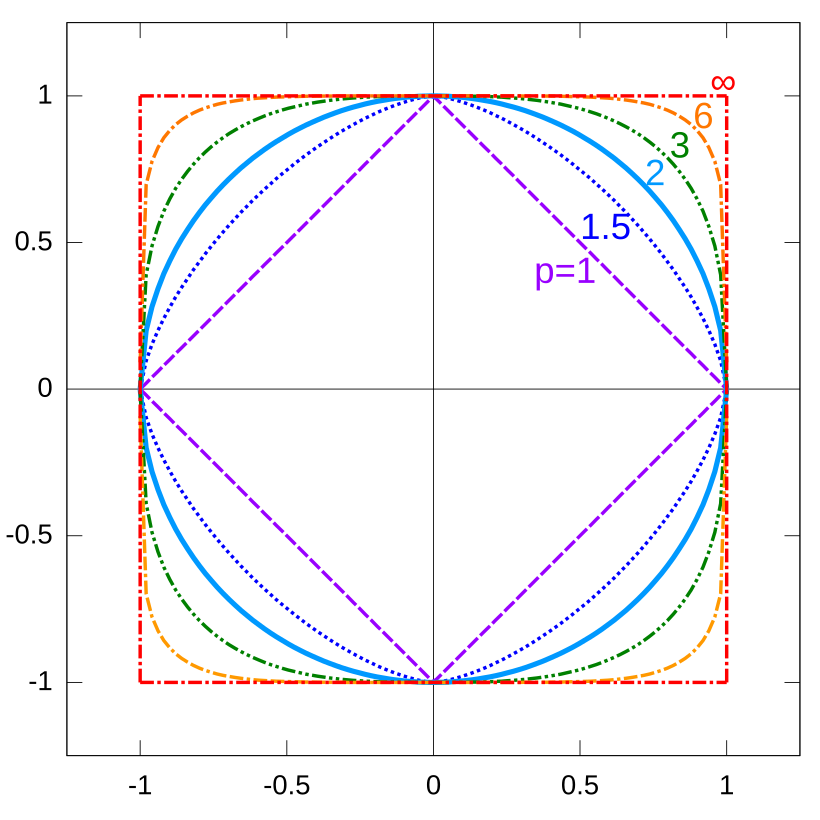
\includegraphics[trim={0 0 0 0}, clip, width=0.4\linewidth]{img/chapter_3/p_norms.png}
    \caption{Various unit balls associated to a $p$-norm in $\mathbb{R}^2$ (from Wikipedia).}
    \label{fig:pnorms}
\end{figure}

% \paragraph*{Symmetric convex sets and $p$-unit balls.}
% In figure \ref{fig:pnorms}, we can see that the most convenient $p$-norm to work with is $p=2$, the euclidean norm: the notion of size in the considered space is the same in any direction (all directions matter). If we consider $p=\infty$, then we are saying that only the principal direction of a vector matters (\emph{i.e.} its largest component in absolute value). Generalizing these interpretations for $2< p <\infty$, the more large $p$ gets, the more importance is given to the principal direction of a vector. A contrario, the more close to $2$ $p$ gets, the less distinction we make between important directions. This is geometrically represented by \emph{how rounded} the unit ball $\mathcal{B}_p^n$ is, with $\mathcal{B}_2^n$ being a purely rounded ball of radius 1 in $\IRn$ and $\mathcal{B}_{\infty}^n$ being a $n$-dimensional cube centered at origin whose edges are of length $2$. Unit balls $\mathcal{B}_p^n$ are necessarily symmetric around the origin of $\IRn$.

% The point of view we are giving to the reader is thus the following: studying $p$-norms of $\IRn$ corresponds to studying the symmetric convex set associated to their unit balls. This is interesting in theory, but there is not much we can do with this.

\paragraph*{Operators.} 
Let $X$ and $Y$ be Banach spaces with norms $\|\cdot\|_X$ and $\|\cdot\|_Y$ respectively. An \emph{operator} $T\,\colon X\rightarrow Y$ is a continuous linear map between $X$ and $Y$. Operators transform Banach spaces into Banach spaces. Linearity ensures that a vector space is mapped to a vector space, and continuity preserves the notion of completeness (\emph{i.e.} the returned space after the transformation has no hole).

If $X$ and $Y$ are finite-dimensional, any operator $T\,\colon X\rightarrow Y$ can be represented in a matrix form. However, this matrix representation only encodes how $X$, as a vector space, is transformed under the map. We require a more powerful tool which allows to study how the norm of $X$ is transformed under $T$. Fortunately, the norm structure $X$ is described as the unit ball of $X$, so we only need to ask ourselves \emph{how does the unit ball of $X$ is transformed through $T$?}. 

This requires more knowledge on $T$. An operator $T\,\colon X\rightarrow Y$ is said to be \emph{bounded} if $T(\mathbf{x})$ is bounded for all $\mathbf{x} \in \mathcal{B}_X$. Since any linear map between normed spaces is continuous if and only if it is bounded, then the operator $T$ is bounded. This implies that the set of operators from $X$ to $Y$ is also a Banach space which can be equipped with a norm called the \emph{operator norm}. It is defined as follows
$$\|T\|_{op} = \sup\left\{\|T(\mathbf{x})\|_Y\mid \mathbf{x}\in \mathcal{B}_X \right\}$$

The direct interpretation of the operator norm is the following: if we consider the unit ball of $X$ and apply $T$ on it, it returns the largest distance between the transformed ball $\{T(\mathbf{x}) \mid \mathbf{x}\in \mathcal{B}_X\}$ and the unit ball of $Y$, as shown in figure \ref{fig:operator_norm}.
\begin{figure}[!htb]
    \captionsetup{justification=centering}
        \centering
        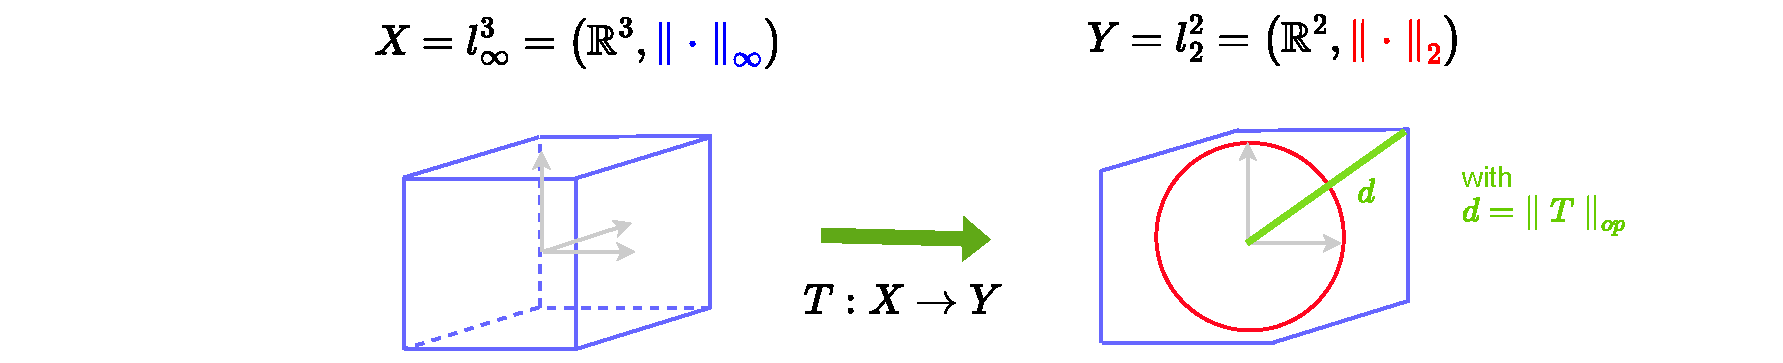
\includegraphics[trim={150 0 70 0},clip, width=1\linewidth]{img/chapter_3/operator_norm.pdf}
    \caption{Geometric interpretation of the operator norm. $T$ projects $\ell_{\infty}^3$ onto $\ell_2^2$, so its norm $\|T\|_{op}$ is the maximal euclidean norm of the vectors describing the surface of the projected unit ball of $\ell_{\infty}^3$. Here, this corresponds to the surface of a zonotope (in blue). This is equivalent to compute in this case the maximal $2$-norm of the zonotope vertices.}
    \label{fig:operator_norm}
\end{figure}

To conclude, the operator norm quantifies the maximal deformation of the transformed unit ball of $X$, relatively to the unit ball of $Y$. We are now fully equiped to dive into the comparison of centrally symmetric convex sets.

\paragraph*{Banach-Mazur distance.} Let's consider two isomorphic Banach spaces $X$ and $Y$, \emph{i.e.} there exists an invertible linear map between $X$ and $Y$. We recall that two finite dimensional real vector spaces are isomorphic if and only if they have the same dimension. In this case, their \emph{Banach-Mazur distance} is defined as 
$$d_{BM}(X,Y) = \inf\{\|T\|_{op} \|T^{-1}\|_{op} \mid T\,\colon X\rightarrow Y \text{  is an isomorphism}\}$$

If $X$ and $Y$ are not isomorphic, we define $d_{BM}(X,Y) = +\infty$.
If the Banach-Mazur distance is $1$, then $X$ and $Y$ are said to be \emph{isometric} (they have the same metric up to isomorphism). In other words, this means that the set of points with a distance of $1$ from the origin in $X$ will correspond exactly to the set of points with a distance of $1$ from the origin in $Y$. More generally, Milman recalls in \cite{milmanDvoretzkyTheoremThirtyYearsLater1992} that for two real finite dimensional spaces $X$ and $Y$ of same dimension with respective unit balls $\mathcal{B}_X$ and $\mathcal{B}_Y$, if $d_{BM}(X,Y) \leq d$, then there is an operator $T\,\colon X\rightarrow Y$ such that
$$\mathcal{B}_X\subset T(\mathcal{B}_Y)\subset d\cdot \mathcal{B}_X$$

This formulation implies that a linear transformation of the unit ball of $Y$ can be encapsulated in between the unit ball of $X$ and its dilation by a factor $d$. In this whole chapter, we will be interested in considering the unit ball of $X$ as an ellipsoid (so $X = l_2^n$) such that the space $Y$ (corresponding to the muscle tension space, or the Cartesian force space) has its unit ball encapsulated by an ellipsoid with $d$ the closest possible to $1$.  

\begin{figure}[!htb]
    \captionsetup{justification=centering}
        \centering
        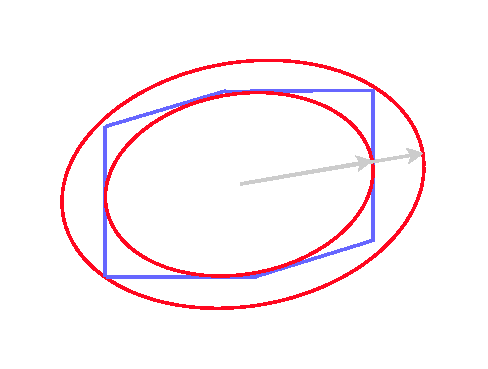
\includegraphics[trim={0 25 0 25},clip, width=0.5\linewidth]{img/chapter_3/banachmazurdvoretzky.pdf}
    \caption{Following figure \ref{fig:operator_norm}, here we can see that the projected zonotope is in between a transformation of the disk (so it is an ellipsoid) and a dilation of this ellipsoid by $1.4$. This means that $d_{BM}(Y, T(X)) \leq 1.4$.}
    \label{fig:banach_mazur_example}
\end{figure}

The Banach-Mazur distance is an entirely theoretic tool: it can not be computed explicitely in most cases. Fortunately, it will be of use in the next sections to show strong approximation results in high dimensions.

In this summary about Banach spaces, we have enunciated some mathematical tools related to the study of a specific class of convex sets: the centrally symmetric sets. Studying convex sets through a more structural approach led to interesting results that we shall describe in the following sections. With the only assumption that the tension set is symmetrically convex, we will show that the \emph{shape} of the force feasible set does not depend on the modeling choice of the tension set, but its \emph{size} does.

Using the \emph{Local Theory of Banach spaces}, section \ref{sec:ellipsoidal_shape_ffs} argues that the shape of the force feasible set is predetermined to be almost an ellipsoid due to its geometric construction. However in practice, there is a need to compute this ellipsoidal shape. Through the \emph{Projection Constant Theory}, section \ref{sec:projected_volume_problem} explitely gives a computational tool to approximate the force and torque feasible set as ellipsoids while considering volume issues related to deforming a norm.

% require more depth, in particular results in what it called the \emph{local theory of Banach spaces}, which focuses on studying infinite-dimensional Banach spaces using only finite-dimensional tools. In particular, we are interested in a major result stating that a specific geometric construction over an initial symmetrically convex set will lead to an ellipsoidal shape.

% , section \ref{sec:ellipsoidal_shape_ffs} will show that due to its geometric construction, the force feasible set has a high probability of resembling an ellipsoid. This result is fundamental because it applies \emph{whatever the choice of the tension set shape}. Even better, this ellipsoidal shape \emph{has to} occur due to the small dimensions of the Cartesian force space and the torque space (which is very different from the other perspective on saying that it occurs du to the large amount of muscles). Section \ref{sec:leveraging_the_projected_volume} will dive much deeper in the \emph{projection constant theory}, including a much more theoretical analysis studying problems related to the projection of a physical unit metric onto a subspace. While these sections are underlyingly studying how convex sets are projected and how muscle tensions are deformed onto torques, the final result is a fast explicit computation of the ellipsoidal approximation of the force feasible set.

\section{The ellipsoidal shape of the force feasible set}
\label{sec:ellipsoidal_shape_ffs}
Results in this section are purely theoretical and are the backbone of the \emph{Local Theory of Banach spaces}. They allow a nicer geometric characterization of the force feasible set, without any assumption on the specific tension set $\mathcal{T}$ shape. However, we \emph{do} assume that $\mathcal{T}$ is convex and symmetric. The symmetry assumption will be leveraged in some cases. Thus, we consider various models of the tension set, noted $\mathcal{T}_p$ models, respectively associated to transformations of unit $p$-balls. A $\mathcal{T}_2$ model implies a purely spherical shape to describe how muscle activations can behave as the same time, while a $\mathcal{T}_{\infty}$ model assumes a cubic shape. For the others $\mathcal{T}_p$, theire curvatures are in between a pure sphere-like shape and a cube, such that we can order these models according to how rounded they are as:
$$\mathcal{T}_2 < \mathcal{T}_3 < \dots < \mathcal{T}_{100} < \dots \mathcal{T}_{\infty}$$

The main result of this section concerns the natural \emph{ellipsoidal} shape of the force feasible set, \emph{i.e.} $\mathcal{T}_p \approx \mathcal{T}_2$ for any $p\geq 2$, but also $\mathcal{T}\approx \mathcal{T}_2$ for any tension set as long as it convex and symmetric. We emphasize this shape with the adjective \emph{ellipsoidal} and not simply \emph{ellipsoid}. This means that globally, the force feasible set resembles an ellipsoid but not perfectly. However, it can be approximated by an ellipsoid which will characterize most of the surface shape: our goal is to compute it (\emph{cf.} next section \ref{sec:projected_volume_problem}) but we have to explain how this phenomenon occurs, and the required conditions to apply such an approximation.

Before diving into the hidden mathematics showing this, let's summarize why such an ellipsoidal shape would be of interest. Firstly, it allows a \emph{much} faster explicit expression, since it requires to only describe the length of the major axes as well a center point and an orientation. The required quantity of parameters is much less than for instance using a polytope representation with many vertices and/or many bounding hyperplanes. Secondly, if in any posture the resulting force feasible set resembles ellipsoids, it can be inferred by geometric construction that the torque feasible set and the tension set shape are ellipsoidal as well, using the fact that ellipsoids are closed under affine transformations. In other words, the tension set $\mathcal{T}$ can be modelized as a $\mathcal{T}_2$ model and allow a much more easier understanding of the relationships between muscle activations: only the mean of maximal tension values characterizes the size of the tension set when seen as a sphere.

All of the following results are non-trivial and require basic understanding of Banach spaces concepts. Besides, they are counter-intuitive and difficult to grasp at first sight, due to the high-dimensional spaces involved in them.

This theory corresponds to the study of infinite dimensional normed spaces using only tools from finite dimensional normed spaces. The name of this theory evolved through the past century, from \emph{Local Banach Theory, Asymptotic Finite-Dimensional Analysis} or even \emph{Probabilistic Geometry} to recently become \emph{Asymptotic Geometric Analysis} \cite{artstein-avidanAsymptoticGeometricAnalysis2015}. Whatever the name and approach, it allows to understand how symmetric convex sets can be approximated by other symmetric convex sets. Metrically, it helps us understand how the tension set physical unit $N$ is transformed onto $N\cdot m$, the physical unit of the torque space when a large number of muscles is considered.
For a full survey on what the local banach theory is, the reader is invited to get acquainted with multiple point of views as described in Pietsch's article \emph{What is local theory of Banach spaces} \cite{pietschWhatLocalTheory1999}. A point of view that would correspond to our current context is the following from Tomczak-Jaegermann (page 5) \cite{tomczak-jaegermannBanachMazurDistancesFinitedimensional1989}:
\begin{quote}
    \emph{``A property [...] is called \emph{local} if it can be defined by a quantitative statement or inequality concerning a finite number of vectors or finite-dimensional subspaces."}
\end{quote}

This section focuses on characterizing the force feasible set \emph{shape}, which is a \emph{global} property. Indeed, the whole shape can be described through its curvature, itself studied through a collection of tangents at each surface point. Those amount to an infinite quantity. A local property requires no infinity: the \emph{size} of a vector is a local property and can be computed in a finite amount of steps. Since it applies for any vector of a vector space, the notion of size itself is a local property of the considered space. The Local Theory tries to study global geometric properties from local ones. In our context, it shall help us understand the force feasible shape by the study of deformation of the various notions of size in between spaces.

However, when dealing with infinity, the major difficulty is counter-intuitivity and the impossibility to have a geometric representation. Fortunately, these difficulties occur also in sufficiently high-dimensional spaces. To get prepared for this journey, let's adopt the counter-intuitive paradigm enunciated by Milman and Yifach \cite{milmanRegularRandomSections2021} as:
\begin{quotation}
    \centering
    \emph{``Existence implies abundance''}
\end{quotation}

Loosely speaking, if it can be shown that there \emph{exists at least one} element of a class of objects having a property in a sufficiently high-dimensional space, then all other elements in this class must share this property. Of course, this does not apply to \emph{any} property. However, the Local Theory is based on the fact that the more complex a normed space is, the more Euclidean it seems to be structured. In other words, if a normed space is equipped with a very complex norm, it still has the structure of a very simple space whose norm is defined by an ellipsoid. As we will show at the end of the section, the force feasible set can be rewritten in a specific way to ensure that it shares this ellipsoidal shape property. 

To guide the reader in the next steps, let's chronoligically summarize the stated results in this section:
\begin{enumerate}
    \item { \textbf{1961 Dvoretzky's theorem \cite{milmanDvoretzkyTheoremThirtyYearsLater1992}:} this is the beginning of the Local Theory. It shows that if you consider a large $m$ and an $m$-dimensional centrally symmetric convex set, then there exists at least one projection onto or one intersection with a $n$-dimensional subspace such that the newly created object resembles an ellipsoid. The dimension $n$ depends on how close the approximation is wanted; }
    \item {\textbf{1971 Milman's abundance \cite{milmanAsymptoticTheoryFinite2001}:} Dvoretzky's theorem is an existence theorem. However, Milman showed that it actually applies for any $n$-dimensional subspace with a high probability. The term \emph{high probability} refers to an increasing probability converging to $1$ as $m$ gets large;}
    % \item { \textbf{1975 Larman and Mani's extension to non-central projection or section \cite{larmanAlmostEllipsoidalSections1975a}:} Dvoretzky's theorem concerns subspaces passing through the origin. Larman and Mani extended his result to a $n$-dimensional subspace passing through any interior point of a $m$-dimensional symmetric convex set. More precise results on the resemblance and how to generalize to abundance have been made by Gordon in 1988 \cite{gordonGaussianProcessesAlmost1988};}
    \item {\textbf{1984 Milman's quotient of subspace (QS) theorem \cite{milmanAlmostEuclideanQuotient}:} For centrally symmetric convex set in $m$ dimension, there exists a subspace of dimension $p$ constructed from a projection then followed by an intersection whose shape resembles an ellipsoid. The main goal of this theorem is to show that the ellipsoidal shape depends on $p$, not on $m$. In other words: it is the geometric construction (projection then intersection) which induces the ellipsoidal shape;}
    \item {\textbf{2021 Milman and Yifrach's quotient of subspace abundance \cite{milmanRegularRandomSections2021}:} The original QS theorem is an existence theorem, which has been generalized to show that it applies for any $p$-dimensional subspace with high probability.}
\end{enumerate}

In our thesis context, the two first theorems show that the more muscles are considered, the closer to an ellipsoid the force feasible set must be. These results apply for the torque feasible set as well. The last two theorems are much more relevant. They state that it is not the number of muscles which defines their ellipsoidal shapes: it is a consequence of the geometric construction. However, all of these theorems are not sufficient to create an ellipsoidal approximation. This will be the objective of the next section \ref{sec:projected_volume_problem}. This short result introduction also shows that all stated theorems are \emph{independant} of the choice a specific norm: we do not assume any shape for the tension set, only that it is centrally symmetric convex.

The next paragraphs describe these results and show that indeed the force feasible set geometric construction can be adapted to correspond to the QS theorem. We shall precise that none of the mentionned theorems will have their proofs described, as they are out-of-scope in this thesis. However, we shall give thorough interpretations.

\subsection{The Local Theory of Banach spaces}
\label{subsec:theoretical_results_local_theory}

\begin{theorembox}{Dvoretzky's Theorem \cite{milmanDvoretzkyTheoremThirtyYearsLater1992}}{dvoretskystheorem}
    For each $\varepsilon > 0$, there is a number $\eta(\varepsilon)>0$ with the following property. Let $E$ be a finite-dimensional Banach space of dimension $m$. Then $E$ contains a subspace $F\subset E$ of dimension $n=\eta(\varepsilon)\log m$ such that $$d_{BM}(F, \ell_2^n) \leq 1+\varepsilon$$
\end{theorembox}
\begin{proof}
    The initial proof has been developped by Dvoretzky himself and is restated in \cite{milmanDvoretzkyTheoremThirtyYearsLater1992}. One approach can be found as the whole Chapter 4 of Pisier's 1989 book about the geometry of Banach spaces \cite{pisierVolumeConvexBodies1989}.
\end{proof}

A direct geometric interpretation of Dvorezsky's theorem is that if we consider a very high (but finite) dimensional normed space $E$ such that $\dim E = m$, then we can always find a normed subspace $F$ of dimension $n$ such that the unit ball of $E$ intersected by or projected onto $F$ is as close as wanted to an ellipsoid. 

Milman conjectured in \cite{milmanDvoretzkyTheoremThirtyYearsLater1992} that for a fixed $n$, we have $m\sim \left(\frac{1}{\varepsilon}\right)^{n/c}$ with $c\sim 2$. Under his hypotheses, the required number of muscles $m$ required such that the torque feasible set in $7$ dimensions \underline{could} have a reasonnable ellipsoidal shape (let's say its Banach-Mazur distance from $\ell_2^7$ is $1.3$) would be $m \sim (1/0.3)^{7/2} \sim 68$ muscles. If we want a better approximation, for $\varepsilon = 0.2$ we would need $m\sim 280$ muscles; for $\varepsilon = 0.1$ then $m\sim 3163$ muscles; and for a very accurate ellipsoid shape assume $\varepsilon = 0.001$, we would need $31622776602$ muscles. These numbers do not take into account the geometric construction of the force feasible set, so the required number of muscles might be \emph{much} lower than these computed bounds.

However, Dvoretzky's theorem is an \emph{existence} theorem, it does not tell us much about how to construct such a subspace $F$. A much stronger result is enunciated with the following theorem due to Milman.
\begin{theorembox}{Milman's abundance \cite{milmanAsymptoticTheoryFinite2001}}{milmantheorem}
    Let $E$ be a finite dimensional Banach space of dimension $m$. Then, any $n$-dimensional subspace $F$ of $E$ has a probability of $1-c(\varepsilon, k, m)$ of having a distance $d_{BM}(F, \ell_2^n) \leq 1 + \varepsilon$, with $\lim_{m\to \infty} c(\varepsilon, k, m) = 0$ for $\varepsilon$ and $k$ fixed.
\end{theorembox}
\begin{proof}
    % The proof is a few dozens of pages long, so we shall only summarize it in a few sentences. The idea is to consider a $n$-dimensional subspace $F$ of $E$ intersecting the unit ball of $E$. Milman used the \emph{concentration of measure phenomenon} which states that in high dimension the majority of the volume of a sphere is located all around an equator. This is a counter-intuitive phenomenon: loosely speaking, it says that most point of sphere are present around a chosen equator, even though we choose any equator. In other words, Milman intersects a high-dimensional unit ball with a lower-dimensional subspace and studies how the newly created points are reparted. He then considers the $n$-dimensional equator passing through these points and show that it can not be very far from the points using the concentration phenomenon. He then computes the volume between an equator and the intersection of a randomly chosen subspace with the unit ball. Now, the notion of volume is strongly related to the notion of measure, itself representing what we usually call \emph{probability}.

    This theorem is actually hidden in Milman's alternative proof of Dvoretsky's theorem and is described in Milman's own book about the Local Theory \cite{milmanAsymptoticTheoryFinite2001}. For a more intuitive approach of the proof, Pisier gives extensive explanations with geometric reasonning of Milman's approach in chapters 2, 7 and 8 of his book \emph{The Volume of convex bodies and Banach space geometry} \cite{pisierVolumeConvexBodies1989}. 
    Also, more insights can be found in the recent survey book \emph{Asymptotic Geometric Analysis, Part I} from Arstein-Avidan, Giannopoulos and Milman \cite{artstein-avidanAsymptoticGeometricAnalysis2015}, especially in chapter 5 for everything related to Dvoretky's theorem and its modern approaches.
\end{proof}

The next theorem is the most fundamental theorem of this chapter. Unfortunately, it is also the most difficult to grasp in this whole thesis. It states that a centrally symmetric convex set intersected with a subspace then orthogonally projected onto a lower subspace has an ellipsoidal shape. The true power hidden in this result resides in the dependency on such approximation can happen: it is the product of the geometric construction, and not necessarily the fact that we consider a high-dimensional space in the first place. However, the theorem is not enunciated this way and requires to understand the notion of \emph{quotient space}.

\paragraph*{Quotient spaces.} Quotient spaces are recurrent mathematical abstract objects appearing in almost all theories. They are usually first encountered in the context of modulo to represent, for instance, how hours are structured on a clock (this is the study of $\mathbb{Z}/12\mathbb{Z}$). We \emph{urge} the reader to not consider any such modulo representation in this thesis context: we prefer a more geometric point of view. Almost everything created in modern mathematics is based on operations on \emph{sets}, through a formalism called the Set Theory. Usually, a particular branch of mathematics will try to express classical operations of sets (union, intersection) into another more adequate form. For instance, natural numbers addition $a+b$ can be seen as the union of two disjoint set $A\cap B$ such that $A$ contains $a$ elements and $B$ contains $b$. The resulting set contains $a+b$ elements. Abstracting classic operations as set operations have the major advantage to better deal with the notions of infinity: loosely speaking, an infinite union of subsets of $\mathbb{N}$ is also a set, while adding infinitely integers returns $+\infty$ which is not necessarily an integer. So, what was noticed is that set theory allows to create abstract objects such that when an operation is applied on them, it is still structured in the same manner.

In linear algebra, the union operation can be transcribed as the union of two vector spaces. However, it is well-known that if $V$ and $W$ are vector spaces, then $V\cup W$ is not a vector space: we must adapt the union operation to ensure that \emph{structure} is kept. This is why the direct sum $V+W := \{v+w\mid v\in V,\, w\in W\}$ is more adapted. The point made is that most mathematical objects have operations which are based on union and intersection of sets, adapted to \emph{ensure} preservation of an underlying structure, simply because it is easier to deal with. 

But there is one more set operation to not forget: the complementary. Still in the vector spaces paradigm, what could possibly be the notion of complementary? The answer lies in the \emph{quotient} operation. The quotient space $V/W$ corresponds to the vectors in $V$ which are not in $W$, while ensuring these vectors are structured and form a vector space. In a simpler context, this corresponds to the notion of orthogonality. $V/W$ can be seen as all vectors of $V$ orthogonal to $W$. We must insist on stating that ``seeing'' $V/W$ as the orthogonal complement of $W$ in $V$ is a point of view: they are not exactly the same spaces. We want to give the reader a full geometric interpretation of $V/W$ but we should always be very careful when directly manipulating the quotient space. In other words, $V/W$ is a totally abstract object not directly representable, but it can be \emph{identified} (\emph{i.e.} the structure is equivalent) to $V\cap \orth{W}$ where $\orth{W}$ is the orthogonal complement of $W$ in $V$. 

Now, let's consider $E$, $Y$ and $X$ be Banach spaces such that $X\subset Y\subset E$. We will describe geometrically the unit balls of $Y$, $X$ and $Y/X$.
A unit ball of $Y$ can be derived directly from the unit ball of $E$: we intersect $\mathcal{B}_E$ with $Y$ and we have $Y$ equipped with $\mathcal{B}_Y := \mathcal{B}_E\cap Y$. For the ball of $X$, we have $\mathcal{B}_X = \mathcal{B}_Y \cap X = \mathcal{B}_E\cap X$ since $Y\subset E$.
What about the unit ball of $Y/X$? Using Pisier's identification in chapter 1 of \cite{pisierVolumeConvexBodies1989}, the ball of $Y/X$ should not be thought through intersection, but through orthogonal linear projection. This means that if $P_X$ is the orthogonal projection from $E$ to $X$, then the unit ball of $Y/X$ is \emph{identifiable} with $P_X(\mathcal{B}_Y)$. Remember that it is only a point of view. Thus, we have that 
$$\mathcal{B}_{Y/X} \longleftrightarrow P_X(\mathcal{B}_E\cap Y)$$

What matters here is the geometric construction of $Y/X$ ball. It is the intersection of a centrally symmetric convex set followed by an orthogonal projection. The previous theorems stated that we can \emph{always} find $Y/X$ such that its unit ball is as close as wanted from an ellipsoid, under the condition of having $\dim E$ sufficiently large. The next theorem goes \emph{much} further: there exists a ball deriving from such a construction $Y/X$ (intersection then projection) that is close to an ellipsoid, no matter how large the dimension of $E$ is. In other words, the culprit of this ellipsoidal shape is the construction. This result is given in its true form in the two next theorems. 

\begin{theorembox}{Milman's quotient of subspace theorem \cite{artstein-avidanAsymptoticGeometricAnalysis2015}}{milman_quotient_subspace_theorem}
    For each $0<\delta<1$, there is a constant $C = C(\delta)$ such that every $n$-dimensional normed space $E$ admits a quotient of a subspace $Y/X$ (with $X\subset Y\subset E$) with dimension $\dim Y/X \geq \delta n$.
    % Let $E$ be an $n$-dimensional normed space. For every $1\leq k < n$, there exists $X$ a subspace of $Y$ with $\dim(Y/X) = n-k$ and 
    % $$d_{BM}(Y/X, \ell^{n-k}_2) \leq C\frac{n}{k}\log\left(C\frac{n}{k}\right)$$
    % where $C>0$ is an absolute constant.
\end{theorembox}

\begin{theorembox}{Milman and Yifach's abundance theorem \cite{milmanRegularRandomSections2021}}{milman_yifach_abundance}
    Theorem \ref{th:milman_quotient_subspace_theorem} applies for any random quotient space with high probability, and with the same deterministic bounds.
\end{theorembox}

\paragraph*{In practice.} If the force feasible set can be written as an intersection followed by a projection, it may have an ellipsoidal shape without any assumption on how the tension set is explicitely modeled, nor how many muscles are considered. Of course, the more muscles there are, the better the approximation is.


A more structural approach stated by Pisier in \cite{pisierVolumeConvexBodies1989} is the following:
\begin{center}
    \emph{``This surprising result gives the impression that in a number of questions, an arbitrary ball in $\IRn$ should behave essentially like an ellipsoid.''}
\end{center}
We shall translate this in a more physical manner: \emph{under intersection-then-projection onto low-dimensional spaces such as the torque space, the unit metric of the tension set (Newton $N$) is deformed quadratically onto the Newton-meters $N\cdot m$ unit.}

Now, there remains two fundamental questions:
\begin{enumerate}
    \item {\textbf{What about non central intersections/projections?} Dvoretzky's theorem concerns subspaces passing through the origin. Larman and Mani extended his result to a $n$-dimensional subspace passing through any interior point of a $m$-dimensional symmetric convex set in \cite{larmanAlmostEllipsoidalSections1975a}. More precise results on the resemblance and how to generalize to abundance have been made by Gordon in 1988 \cite{gordonGaussianProcessesAlmost1988}. It is a strong limit that the quotient subspace theorem has not yet been generalized to affine maps instead of linear, but it seems in practice that similar phenomenons are still occuring in affine cases;}
    \item {\textbf{To what extent does the force feasible set satisfy the quotient of subspace theorem?} The next paragraphs will show that the force feasible set formulation, initially seen as a projection then intersection problem, can be rewritten as an intersection first followed by a projection.}
\end{enumerate}

\subsection{Rewritting the force feasible set geometric construction}
\label{subsec:rewriting_force_feasible_set}
The following result rewrites the order of the geometric construction of the force feasible set $\mathcal{F}$: instead of the order \emph{projection then intersection}, we have an equivalent description as \emph{intersection then projection}. The key idea is to find the largest dimensional affine subspace $K$ of $\IRm$ such that $K\cap \mathcal{T}$ will directly map to $\mathcal{F}$. In a more meaningful manner, we are showing that the force feasible set is produced from muscle tensions which are linearly constrained, and we explicit these constraints. Note that this can be considered as an extension of Scott et al.'s work on polytopes described as a section of a zonotope, \emph{i.e.} a section of a projection of a cube \cite{scottConstrainedZonotopesNew2016}.
\begin{theorembox}{Rewritting the force feasible set}{convex_section}
    Let $p \leq n \leq m$ be integers and define the linear map $\phi\colon \IRp \rightarrow \IRn$ to be injective of rank $p$ and the affine map $\psi\colon \IRm \rightarrow \IRn$ to be surjective of rank $n$.
    Let $\mathcal{T}$ be a convex set of $\IRm$.
    Then for any non-empty convex set $\mathcal{F}\subset\IRn$ such that $\mathcal{F} = \im \phi \cap \psi(\mathcal{T})$, we have 
    $$\mathcal{F} = \psi(K \cap \mathcal{T})$$
    with $K = \orth{\psi^T(\orth{(\im \phi)})}\subset \IRm$ an affine subspace of dimension $m-(n-p)$, where $\psi^T \colon \IRn \rightarrow \IRm$ defined as $\psi^T(\tau) = -L\tau + (L^T)^+\mathbf{G}$ denotes the \emph{transpose} mapping of $\psi$ and the operator $\orth{A}$ is the orthogonal complement of any subspace $A$. 
\end{theorembox}
\begin{proof}
    This proof is devided into two parts: firstly, let's show that $\psi(K) = \im\phi$ and secondly, show that $\psi(K\cap \mathcal{T}) = \psi(K)\cap \psi(\mathcal{T}) = \im\phi \cap \psi(\mathcal{T}) $ using the result from the first part.

    \underbar{1) $\psi(K) = \im\phi$:}
    This part is proven by construction of $K$ itself. The idea is to find the largest (in dimensions) $K\subset\IRm$ such that the direct sum $K+\orth{K} = \IRm$. Recall that in an euclidean space, we necessarily have $K\cap \orth{K} = 0_{\IRm}$ so that $\dim K + \dim \orth{K} = m$ and consequently $\psi(K+\orth{K}) = \psi(K) + \psi(\orth{K})$.

    For this, we will ensure that $\orth{K}$ is in a one-to-one correspondance with $\orth{(\im \phi)}$: this is one way to ensure the smallest possible dimension for the orthogonal complement of $K$, resulting in $K$ surjecting onto $\im \phi$ and such that $K$ has the largest possible dimension.

    An easily found bijective mapping between the complements can be described by the transpose map $\psi^T$ of $\psi$. In this case, $\psi^T$ is necessarily injective since $\psi$ is surjective, and since the restriction of $\psi^T$ to $\orth{(\im \phi)}$ naturally surjects onto $\psi^T(\orth{(\im \phi)})$, combined with injectivity of $\psi^T$ we have that this restriction is in one-to-one correspondance with $\orth{K}$.

    So let's define $\orth{K} = \psi^T(\orth{(\im \phi)})$. By taking orthogonal complements we have defined $K = \orth{\psi^T(\orth{(\im \phi)})}$ which has the following properties:
    $$\psi(K) = \im \phi \quad \text{and}\quad \psi(\orth{K}) = \orth{(\im\phi)}$$
    
    \underbar{2) $\psi(K\cap \mathcal{T}) = \psi(K) \cap \psi(\mathcal{T})$:}

    This requires recent theoretical results which can be found in Kushnir and Liu 2017's article on linear transformation of union and intersection of convex sets \cite{kushnirLinearTransformationsIntersections}. Let's first define the following:
    a set $C\subset \IRm$ is \emph{convex in direction} $d\in\IRm$ if for all $a, b\in C$ such that $a-b=\alpha d$ for some $\alpha\in \IR$, we have $[a,b]\subset C$.

    \begin{lemmabox}{Theorem 2 from Kushnir and Liu \cite{kushnirLinearTransformationsIntersections}}{kushnir_theorem}
        For a linear transformation $T \colon \IRm \rightarrow \IRn$ and closed convex sets $A$ and $B$ of $\IRm$, if the union $A\cup B$ is convex in every direction $d\in \ker T$, then $T(A\cap B) = T(A)\cap T(B)$.
    \end{lemmabox}

    This result will be applied in the case of $T=\psi$, $A=K$ and $B=\mathcal{T}$. First, $K$ is a closed convex set of $\IRm$ because every Euclidean affine space is closed and convex. $\mathcal{T}$ is a closed convex set of $\IRm$ by definition of $\mathcal{T}$ in this chapter. Now, $\psi$ is not linear: it is affine, so it's a composition of a linear mapping and a translation. It does not invalidate the theorem, as only the linear part can be applied then translate the produced sets. So without loss of generality, let's briefly consider that $\psi$ is linear.

    The key of this proof is that $\ker \psi \subset K$. Firstly, recall that $\ker \psi = \orth{(\im \psi^T)}$ using a classic result relating the four fundamental subspaces generable by a matrix: the column-space of a matrix $A$ equals the orthogonal complement of the null-space of the transpose $A^T$, and the column-space of $A^T$ equals the orthogonal complement of the null-space of $A$. Secondly, we clearly have $K = \orth{\psi^T(\orth{(\im \phi)})} \iff \orth{K} = \psi^T(\orth{(\im \phi)})$ so that $\orth{K}\subset \im \psi^T$. By applying the orthogonal complement in both sides (this requires changing the inclusion order), we obtain
    \begin{align*}
        \orth{(\im \psi^T)} \subset \orth{(\orth{K})} &= K \\
        \iff \ker{\psi} \subset K
    \end{align*}
    To apply lemma \ref{th:kushnir_theorem}, it remains to show that $K\cup \mathcal{T}$ is convex in every direction of $\ker \psi$. Consider $a, b\in K\cup \mathcal{T}$ such that $a-b$ belongs to a $1$-dimensional subspace of $\ker\psi$. Since we previously showed $\ker\psi \subset K$, we naturally have $a-b\in K$. By convexity of $K$, $[a,b]\subset K\subset K\cup \mathcal{T}$ and the lemma can be applied to deduce that $K\cup \mathcal{T}$ is convex in every direction of $\ker \psi$.

    This shows that $\psi(K\cap \mathcal{T}) = \psi(K)\cap\psi(\mathcal{T}) = \im \phi \cap \mathcal{T}$. 
    
    Also, we have 
    \begin{align*}
        \dim \orth{(\im \phi)} &= n - p \\
        \iff \dim \psi^T(\orth{(\im \phi)}) &= n - p \\
        \iff \dim \orth{\psi^T(\orth{(\im \phi)})} &= m - (n-p) \\
        \iff \dim K &= m - (n-p)
    \end{align*}
\end{proof}

Our theoretical result \ref{th:convex_section} showed that force feasible sets are indeed constructed in an intersection then projection pattern. It is sufficient to apply on it Milman's quotient of subspace theorem and confirm its ellipsoidal shape with a high probability. 

As a corollary of this rewritting, there is a surprising biomechanical interpretation of the force feasible set extremal points when using a $\mathcal{T}_{\infty}$ model:
\begin{lemmabox}{Maximal number of muscles fully-activated or not}{maximal_nb_tension_vertex}
    Consider the $\mathcal{T}_{\infty}$ model of the tension set $\mathcal{T}$ of $m$ muscles acting on $n$ joint torques. The force feasible set $\mathcal{F}$ is thus a polytope whose extremal points (vertices) are generated by a tension combination of $m$ muscles. To produce such a combination, there are maximum $n-p$ muscles which are not either fully-activated or not-activated.
\end{lemmabox}
\begin{proof}
    Any vertex of $\mathcal{F}$ is produced from the intersection of a subspace $K$ and a face of the tension set of dimension greater than $m-n+p$. Let's call $F$ such a face and we seek its maximal dimension. We consider a case where $K$ is not parallel to any face of the cube. Since $0$-dimensional intersections (which are points) will map to $0$-dimensional vertices of $\mathcal{F}$, we search for $\dim F$ such that $\dim F\cap K = 0$:
    \begin{align*}
        \dim F\cap K & = \dim F + \dim K - \dim F\cup K \\
        \implies 0 &\geq \dim F + \dim K - m \\
        \implies 0 &\geq \dim F + m-(n-p) - m\\
        \implies n-p &\geq \dim F\\
    \end{align*}

    This means that the tension combinations producing a force polytope vertex are located on some face of the cube $\mathcal{T}$ of dimension less than $n-p$. Hence, there are $m-(n-p)$ coordinates in this combination which are not free (in the mathematical sense): they are either at their minimal or maximal value since this is how the faces of a cube are characterized.
\end{proof}

When considering a large number of muscles, $p=3$ and $n=7$, this implies that to produce a maximal force, each muscle is either fully activated or not activated, and there is only a tiny amount of them which have in-between activations. In this example, this amount is $\leq n-p=4$.

More generally, if $m \gg n$, $m-(n-p) \sim m$, so we could consider that any muscle tension is either fully-activated or not at all. This approximation is however nowhere practical in direct computation since there are always combinatorial issues related to cubes, zonotopes and polytopes, but this result is relevant in showing how the choice of a tension set model can lead to strong biomechanical assumptions. 

\subsection{Ellipsoidal approximation in practice}
\label{subsec:ellipsoidal_approx_in_practice}
While previous theorems allowed us to better understand the force feasible shape, let's compute some $\mathcal{F}$ under a $\mathcal{T}_{\infty}$ model to grasp how it can have an ellipsoidal shape. Since all unit balls $\mathcal{B}_p^m$ for $2 \leq p < \infty$ are inscribed in the unit cube $\mathcal{B}_{\infty}^m$ and also more rounded than the cube, if the force feasible set resulting from a $\mathcal{T}_{\infty}$ model is indeed ellipsoidal, then necessarily all $\mathcal{T}_p$ models would lead to much more correct ellipsoidal approximations (with a $\mathcal{T}_2$ leading to \emph{exactly} an ellipsoid).

Let's consider a first musculoskeletal model with $7$ degrees-of-freedom, with $m = 11$, $20$ or $50$ muscles crossing all joints. This means that the lever arm transpose matrix $-L^T$ has almost no $0$ values in it. Consider a uniformly generated random vector $\mathbf{G}\in \mathbb{R}^7$ representing the gravity torque vectors, whose values range in $[-100,100]$. Likewise, generate uniformly a matrix $-L^T \in \mathbb{R}^{7 \times m}$ with values in $[-1,1]$, a matrix $J^T \in \mathbb{R}^{7\times 3}$ with values in $[-5,5]$. For each muscle, its minimal tension value is defined to be random in $[0,100]$ and its maximal tension value in $[200, 1200]$. This large range allows to consider multiple types of muscles with different maximal forces. The figure \ref{fig:example_ellipsoidal_zonotope_multijoints} shows the produced force feasible sets computed using the \emph{Iterative Convex Hull method} (ICH) from Skuric et al. \cite{skuricOnLineFeasibleWrench2022} with a tolerance of $0.2$, as described in chapter \ref{chapter:2}.

\begin{figure}[!htb]
    \captionsetup{justification=centering}
    \begin{minipage}{1\linewidth}
        \centering
        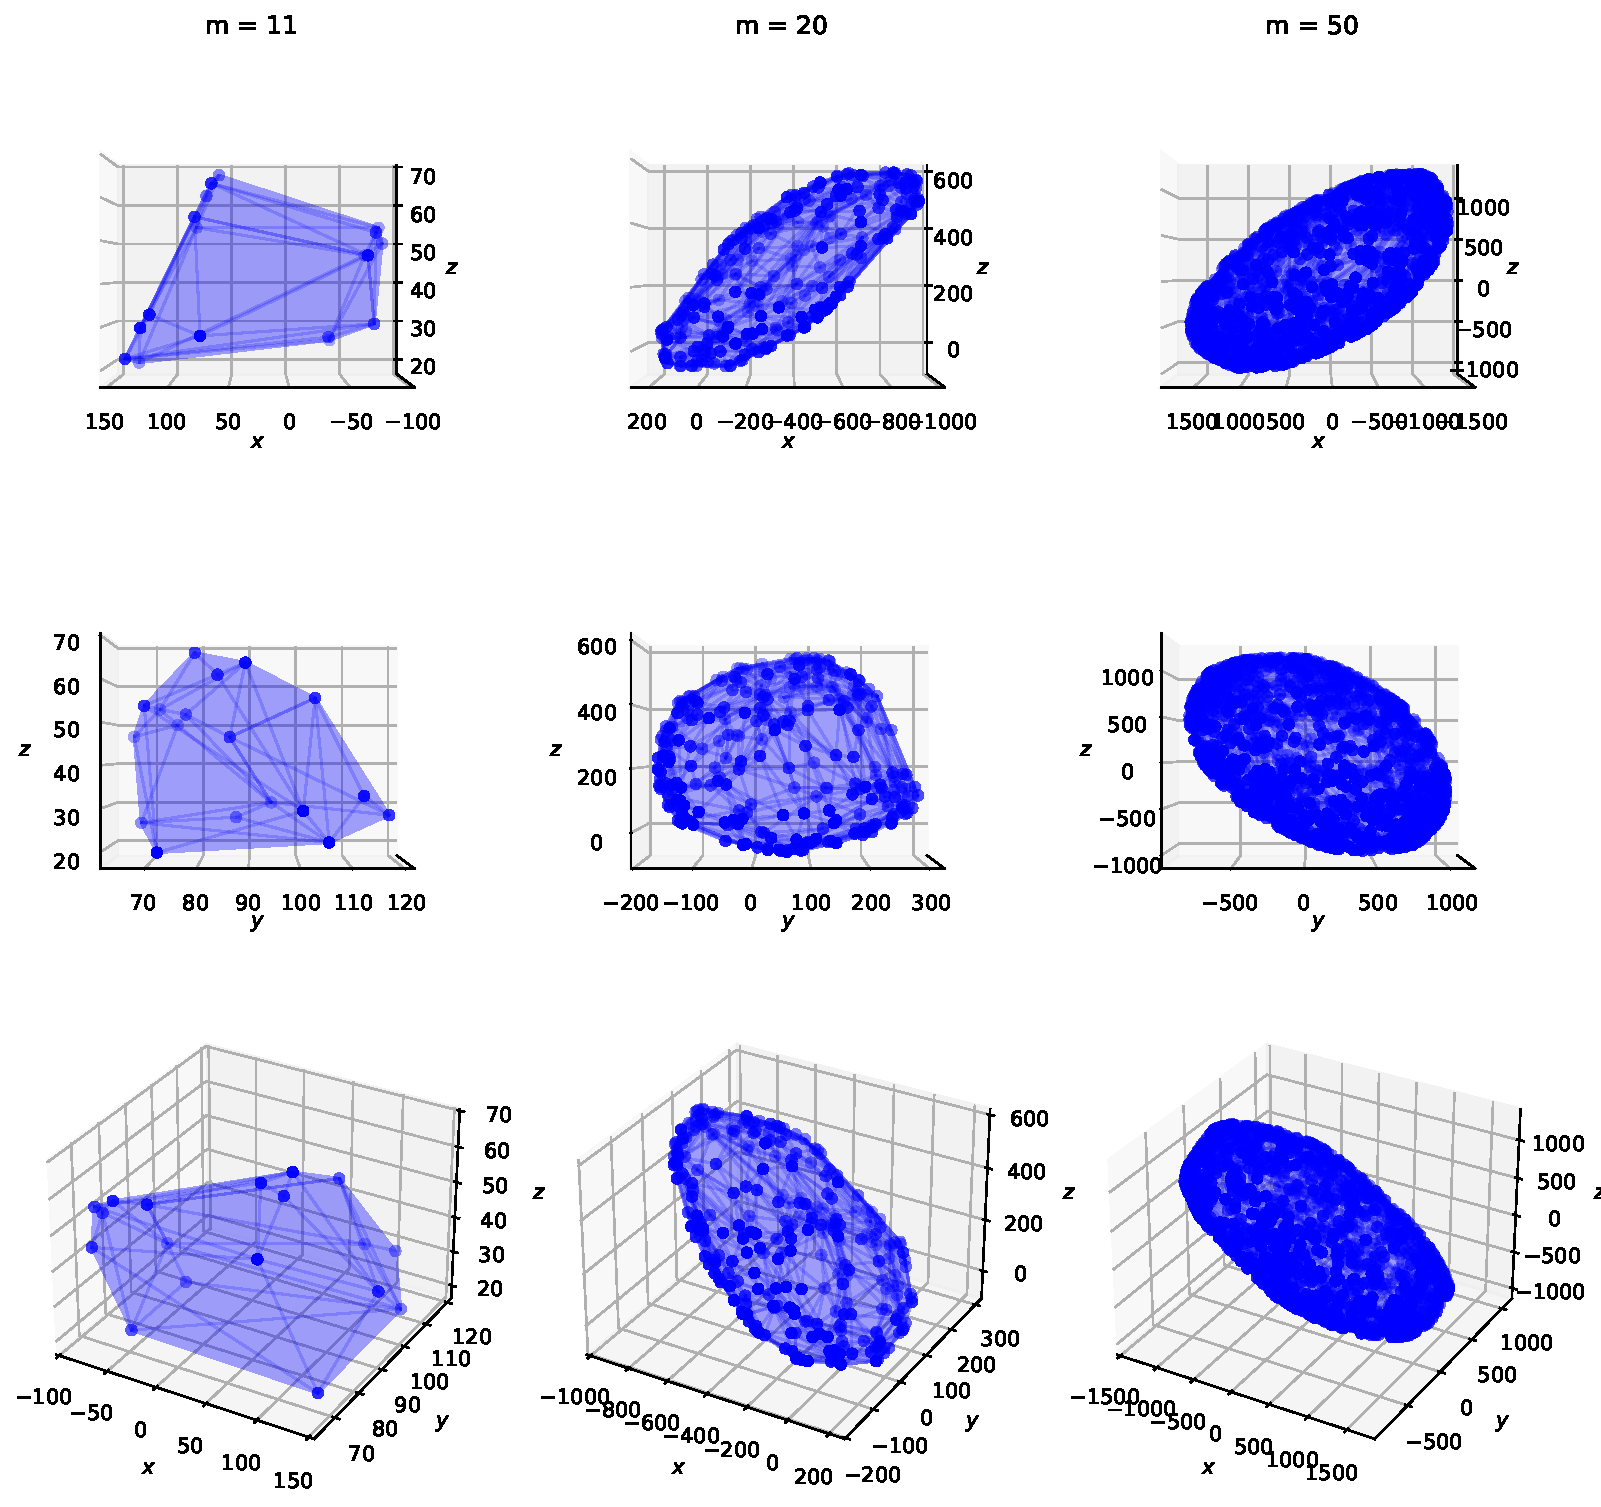
\includegraphics[trim={0 700 0 0},clip, width=0.9\linewidth]{img/chapter_3/zonotopes_looks_like_ellipsoids.pdf}
    \end{minipage}
    \begin{minipage}{1\linewidth}
        \centering
        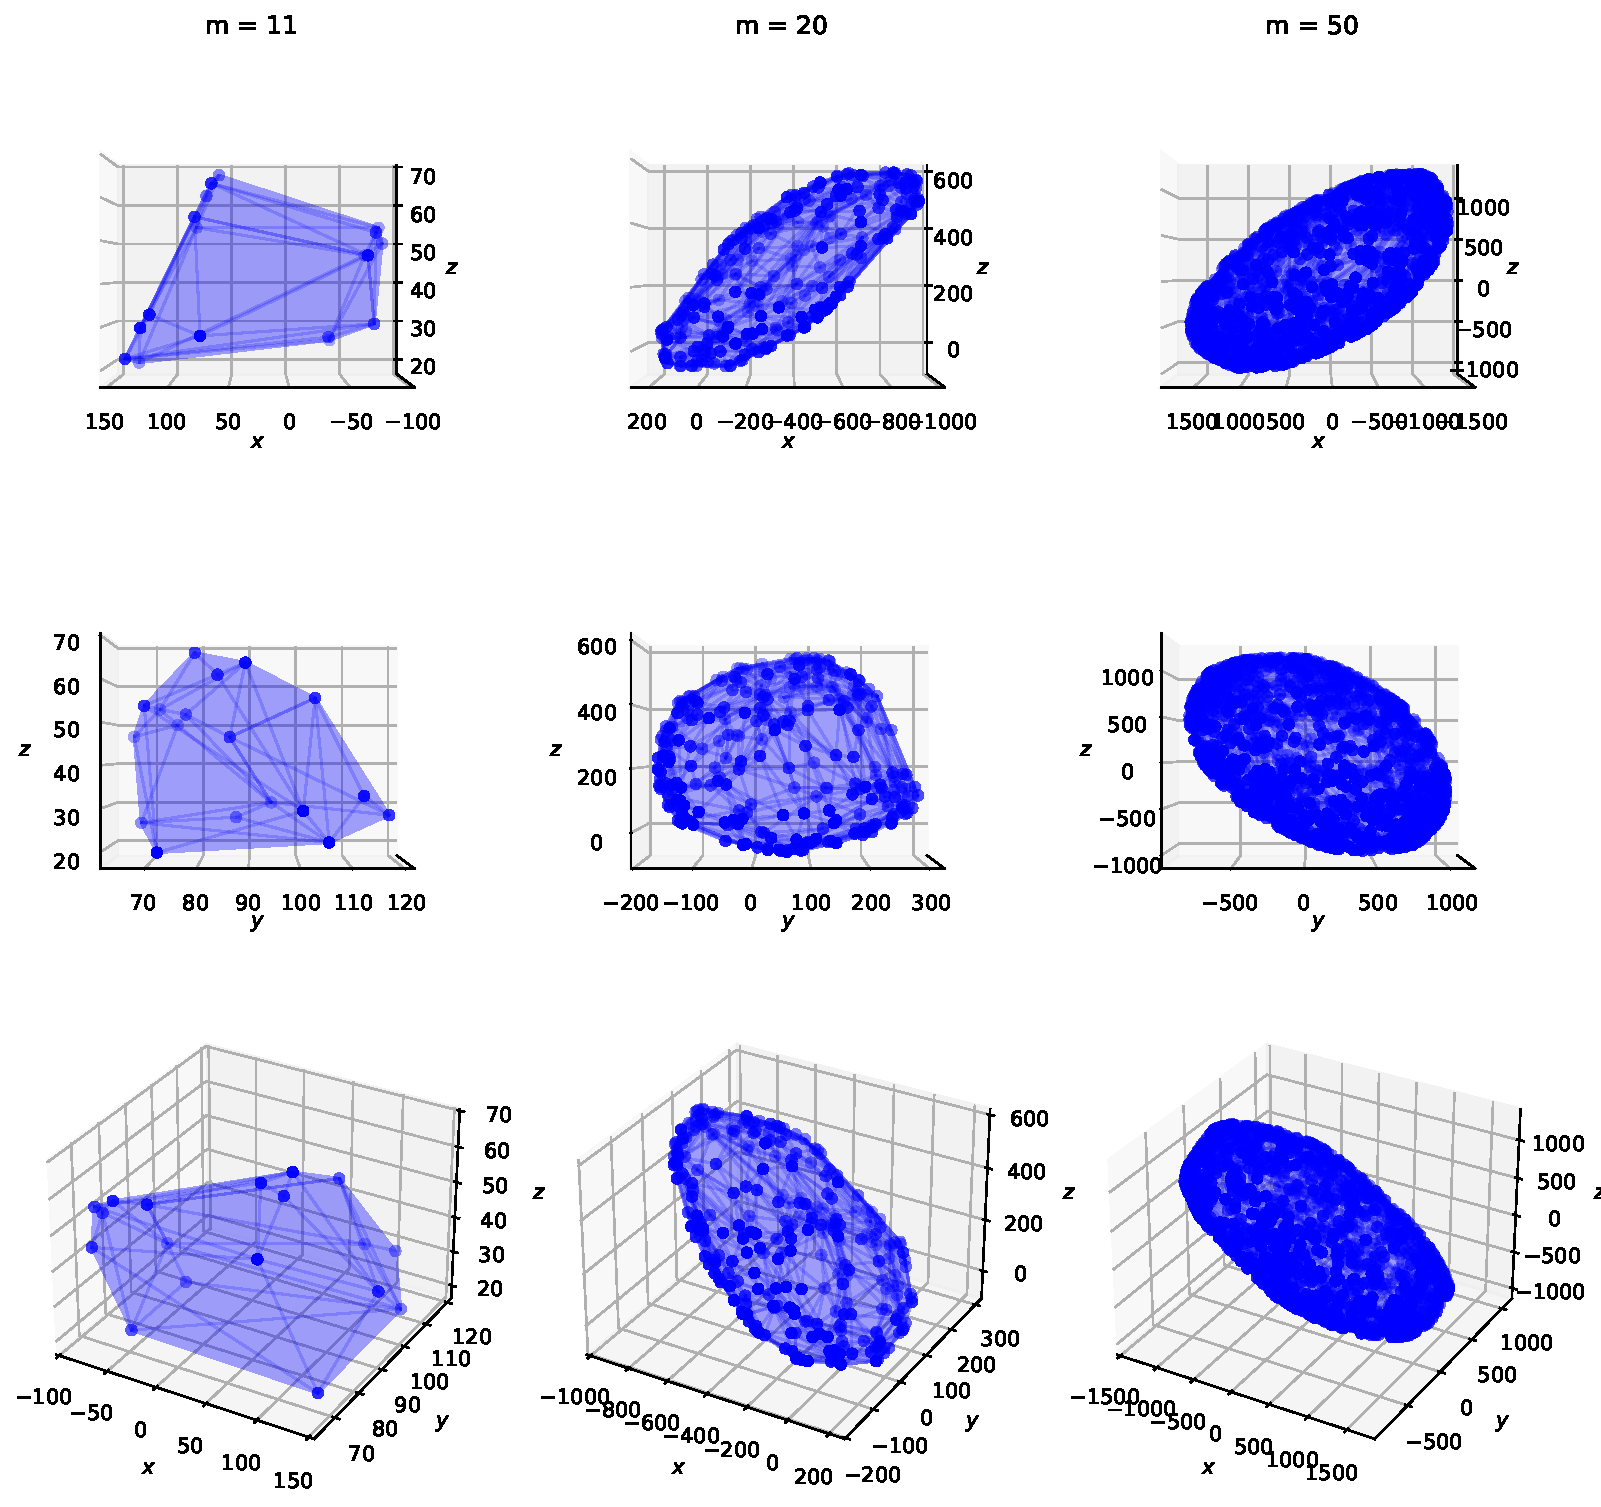
\includegraphics[trim={0 500 0 60},clip, width=0.9\linewidth]{img/chapter_3/zonotopes_looks_like_ellipsoids.pdf}
    \end{minipage}
    \begin{minipage}{1\linewidth}
        \centering
        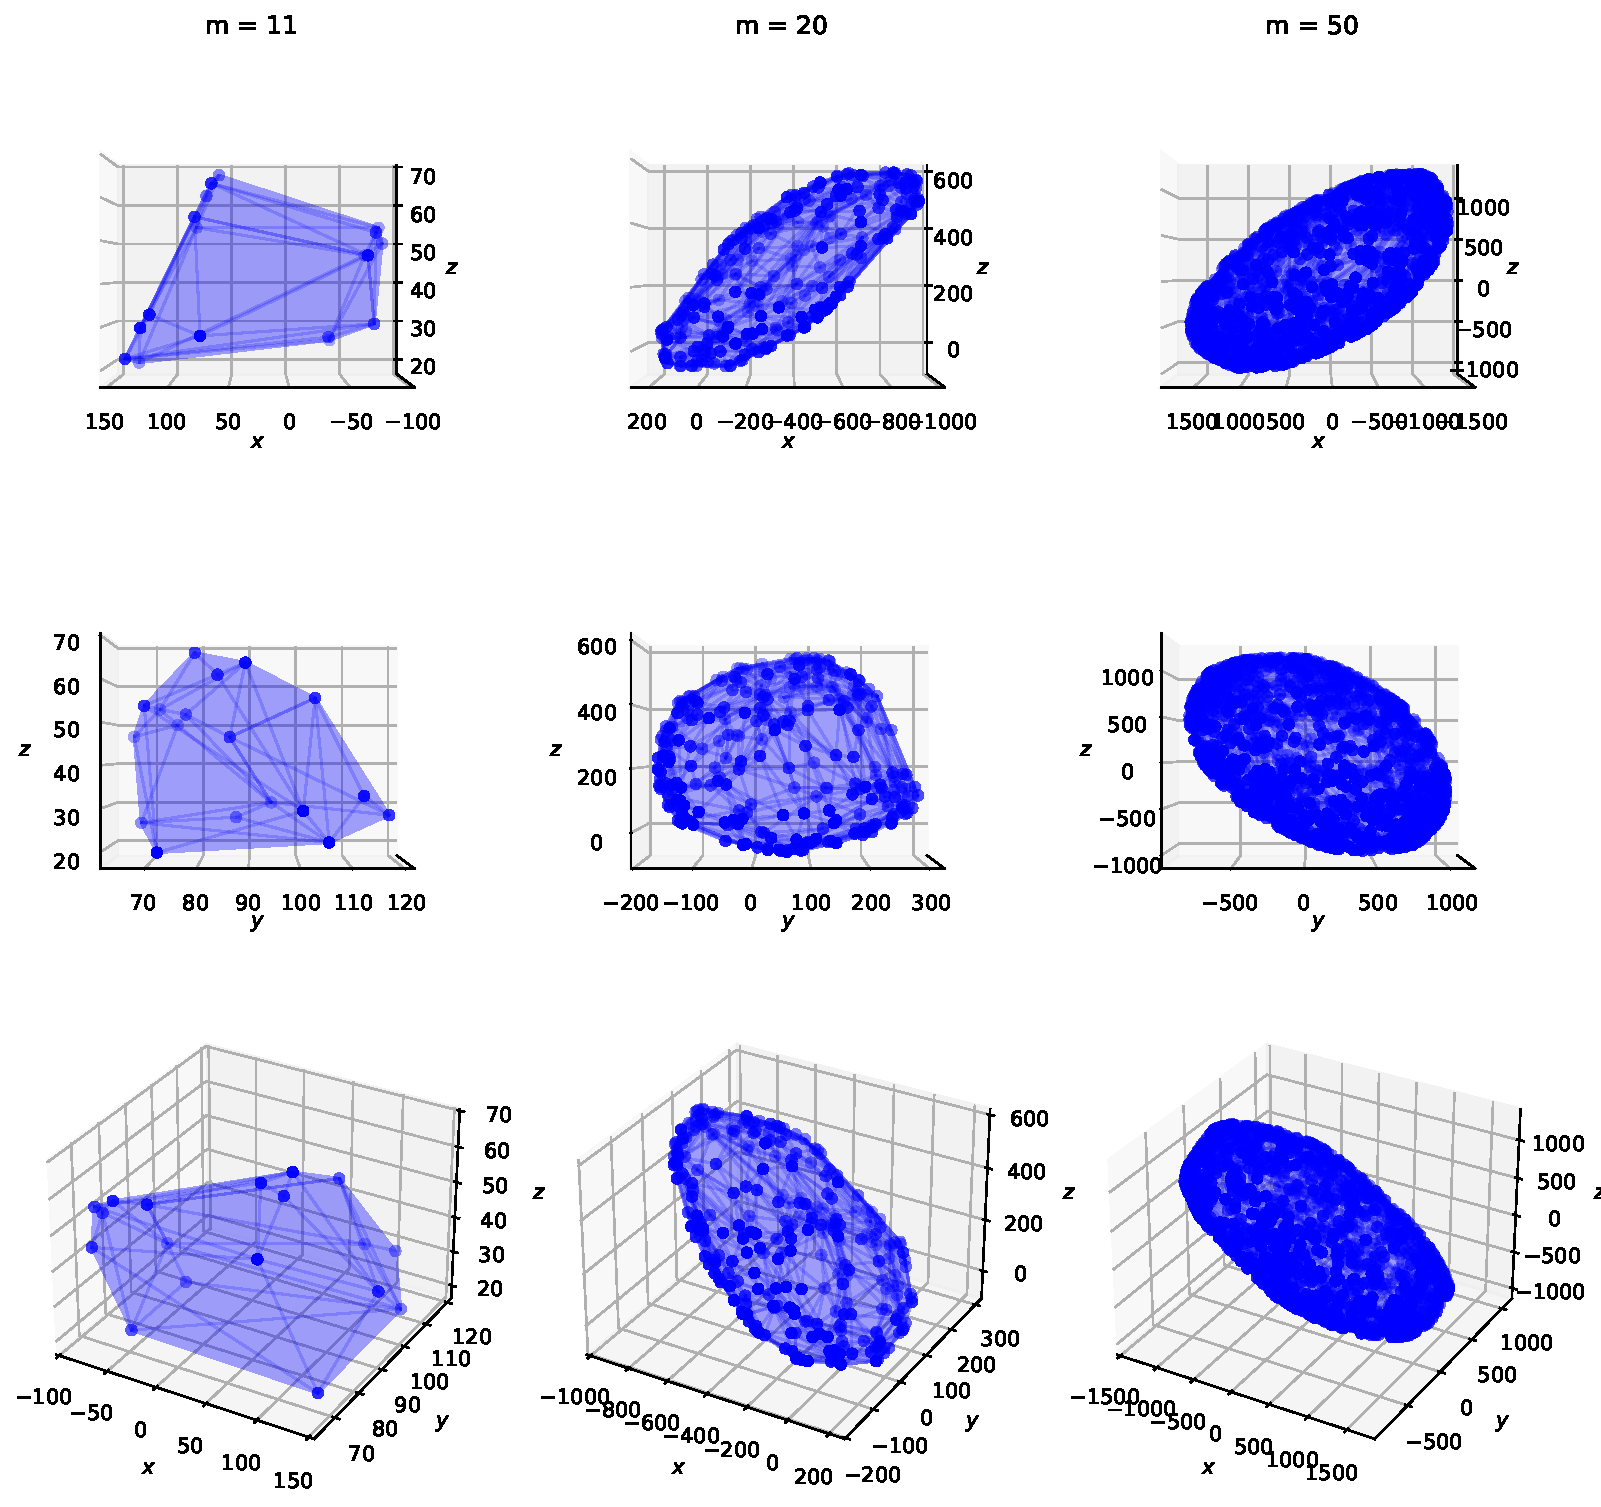
\includegraphics[trim={0 255 0 300},clip, width=0.9\linewidth]{img/chapter_3/zonotopes_looks_like_ellipsoids.pdf}
    \end{minipage}
    \begin{minipage}{1\linewidth}
        \centering
        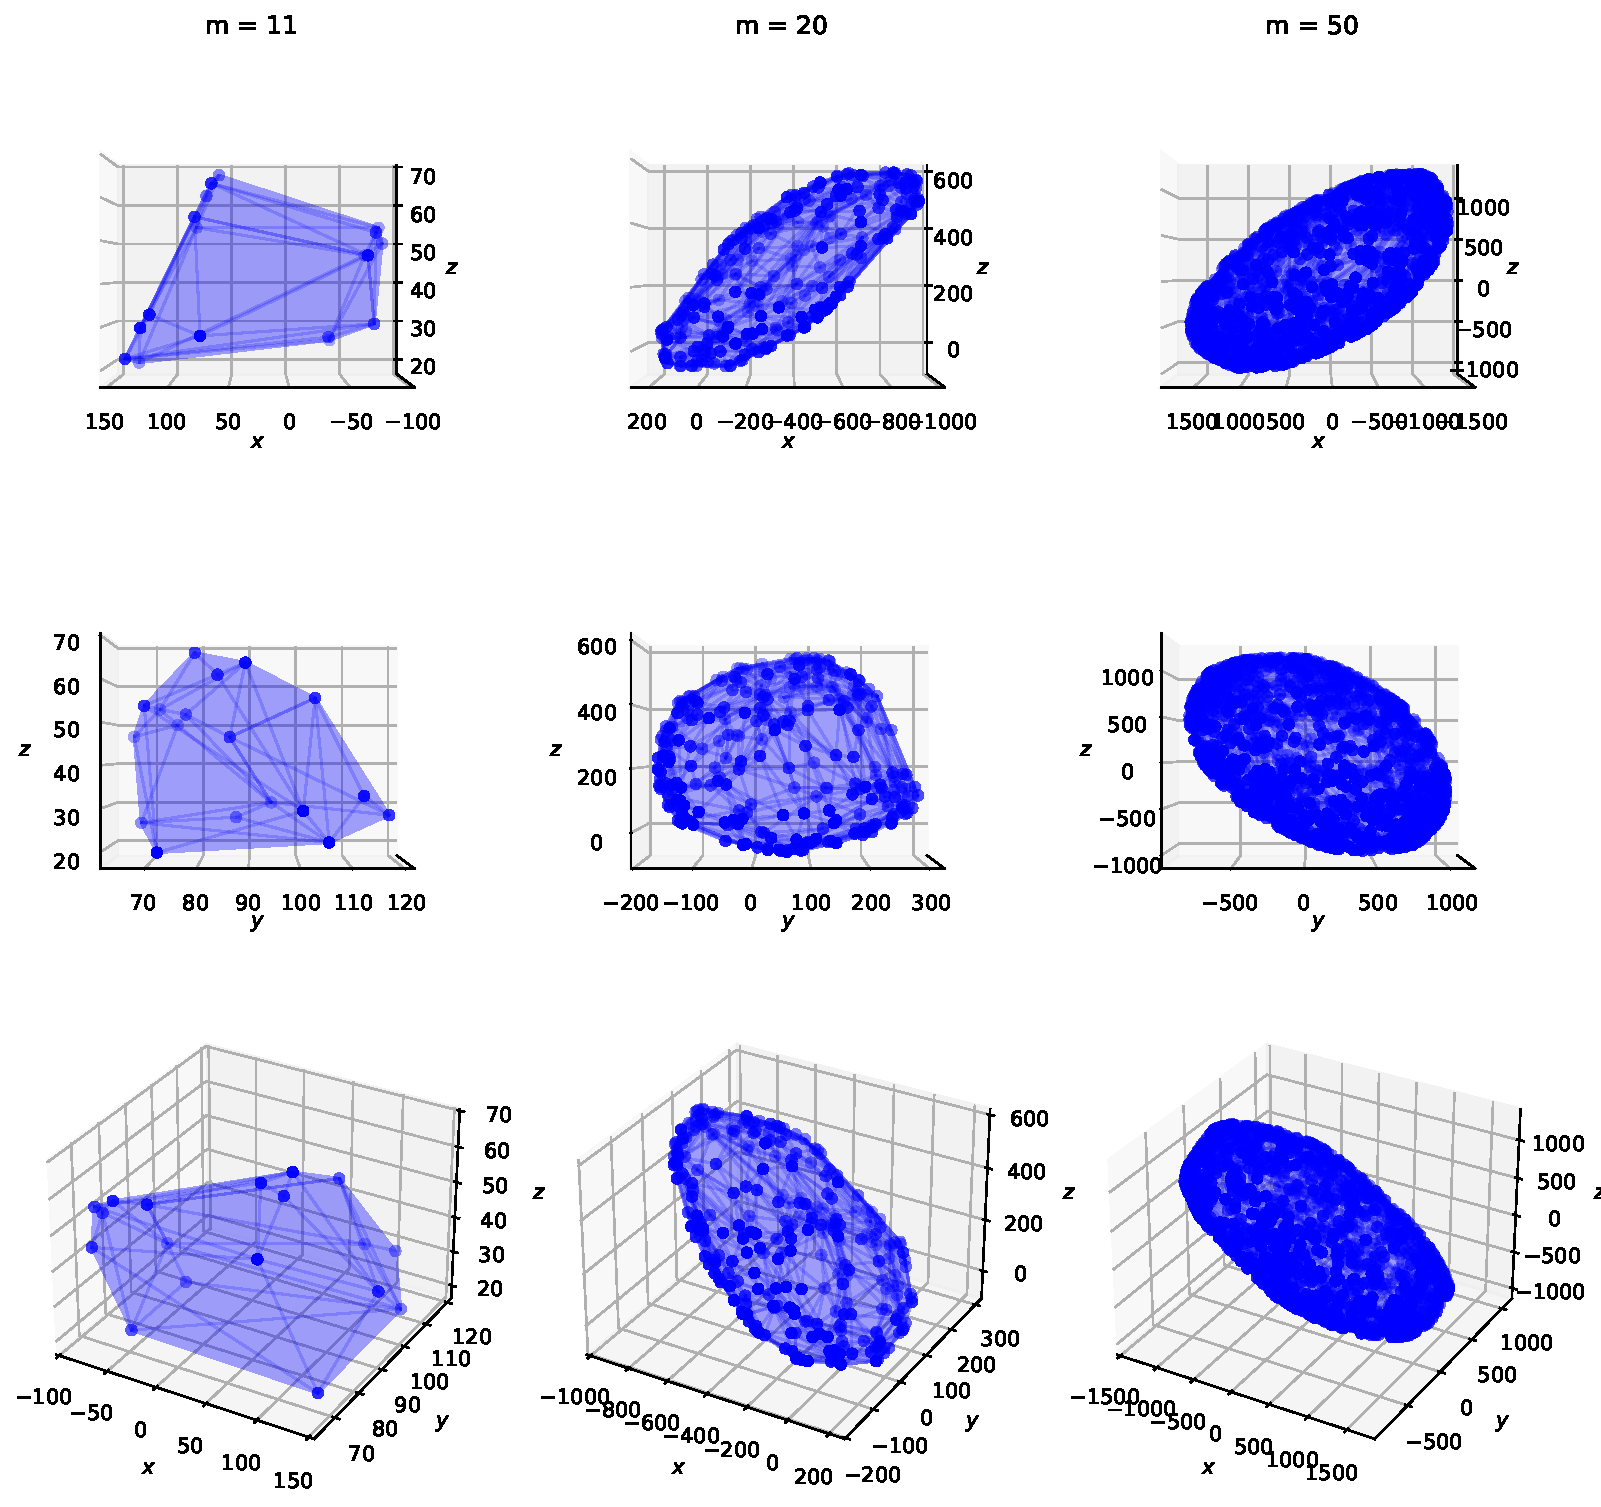
\includegraphics[trim={0 0 0 500},clip, width=0.9\linewidth]{img/chapter_3/zonotopes_looks_like_ellipsoids.pdf}
    \end{minipage}
    
    
    \caption{Each column correspond to a different number of muscles ($m=11$, $20$ and $50$). Each row is a different orientation of the computed force feasible set to better grasp the 3D. 
    Since only the \emph{shape} is of interest in this section, the axes are not the same on each column.Here, the lever arm matrix was considered to be dense (each of its values is different from $0$). This implies all randomly generated muscles act on all of the $7$ joint torques.
    }
    \label{fig:example_ellipsoidal_zonotope_multijoints}
\end{figure}

\begin{figure}[!htb]
    \captionsetup{justification=centering}
    \begin{minipage}{1\linewidth}
        \centering
        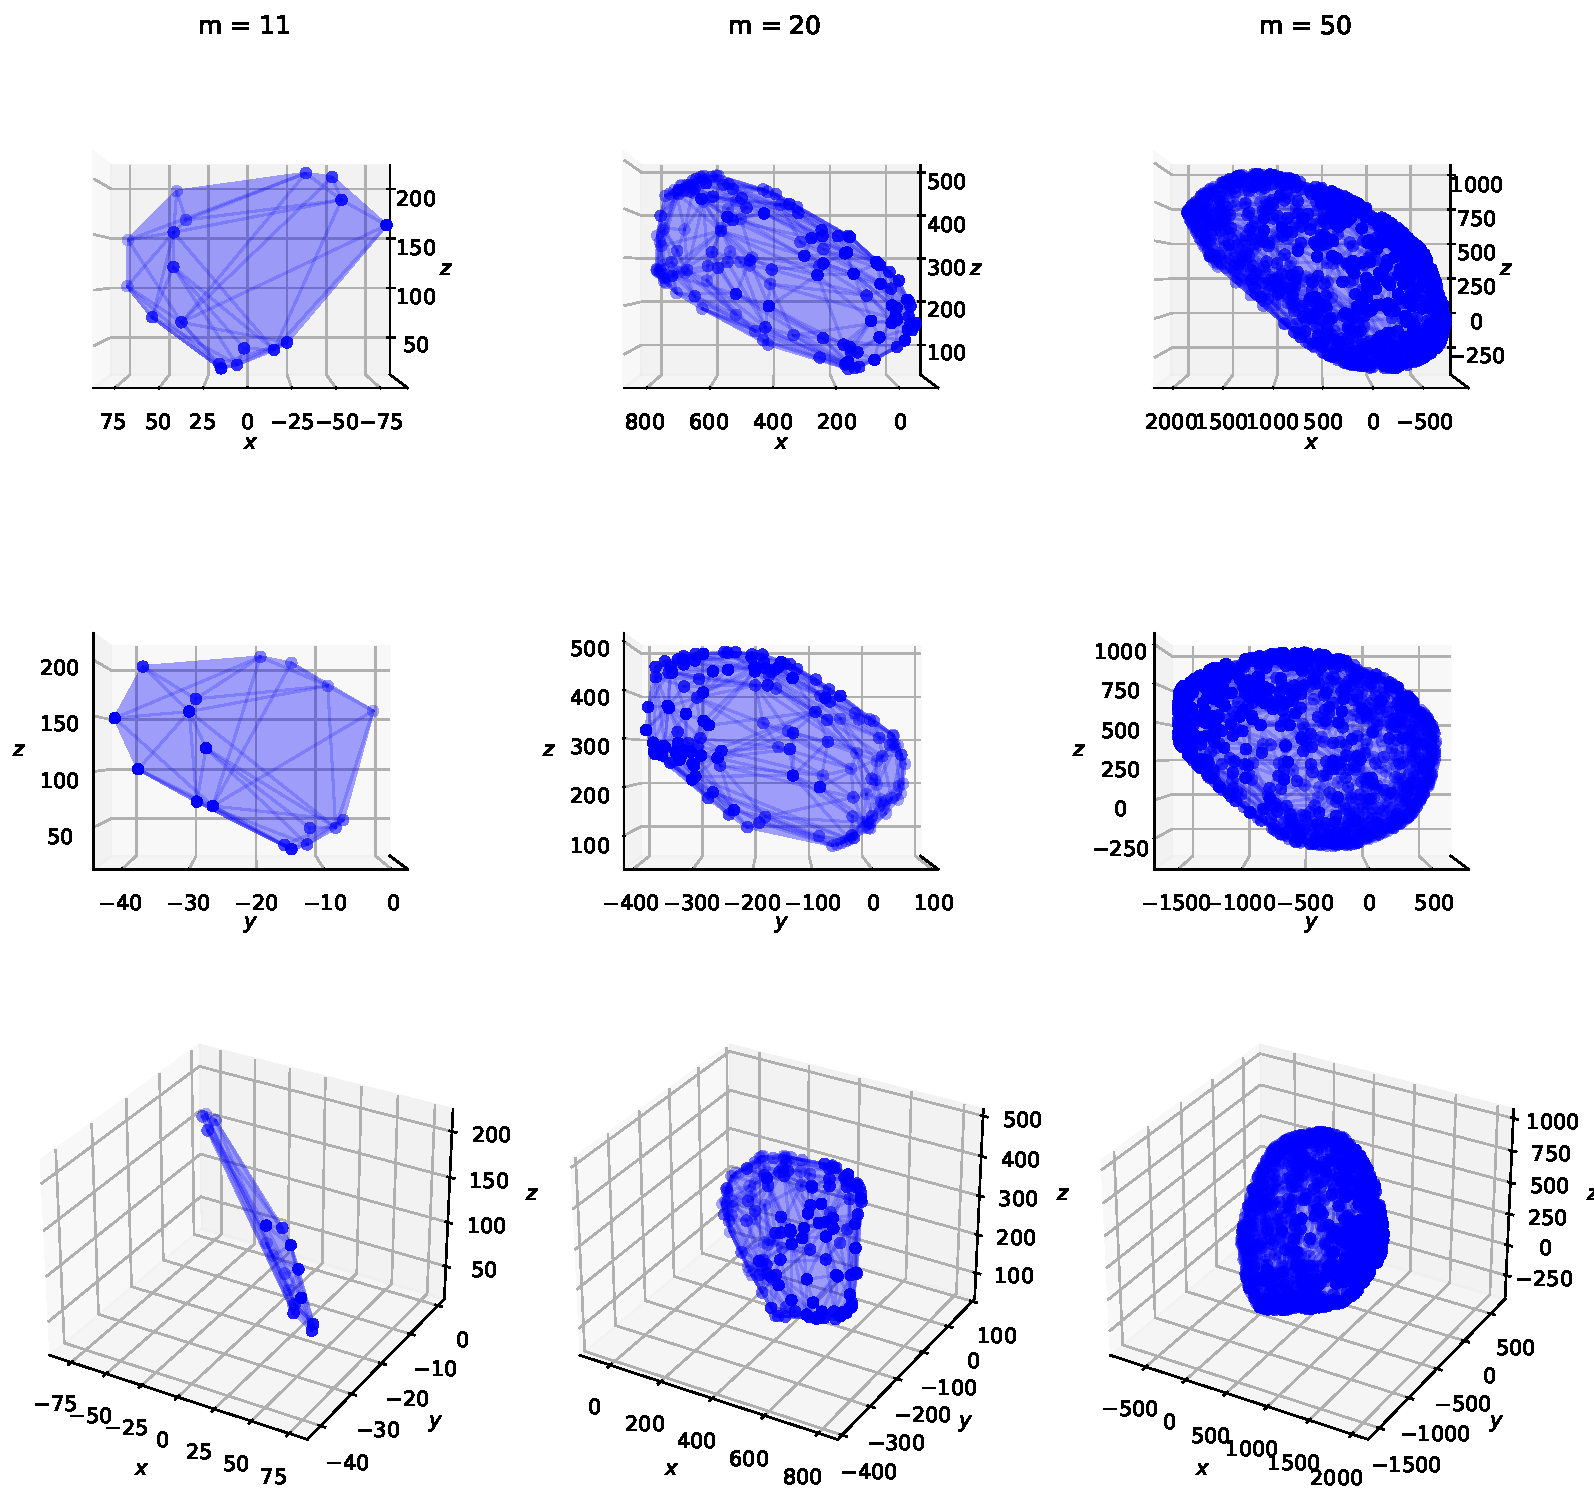
\includegraphics[trim={0 700 0 0},clip, width=0.9\linewidth]{img/chapter_3/zonotopes_looks_like_ellipsoids_2.pdf}
    \end{minipage}
    \begin{minipage}{1\linewidth}
        \centering
        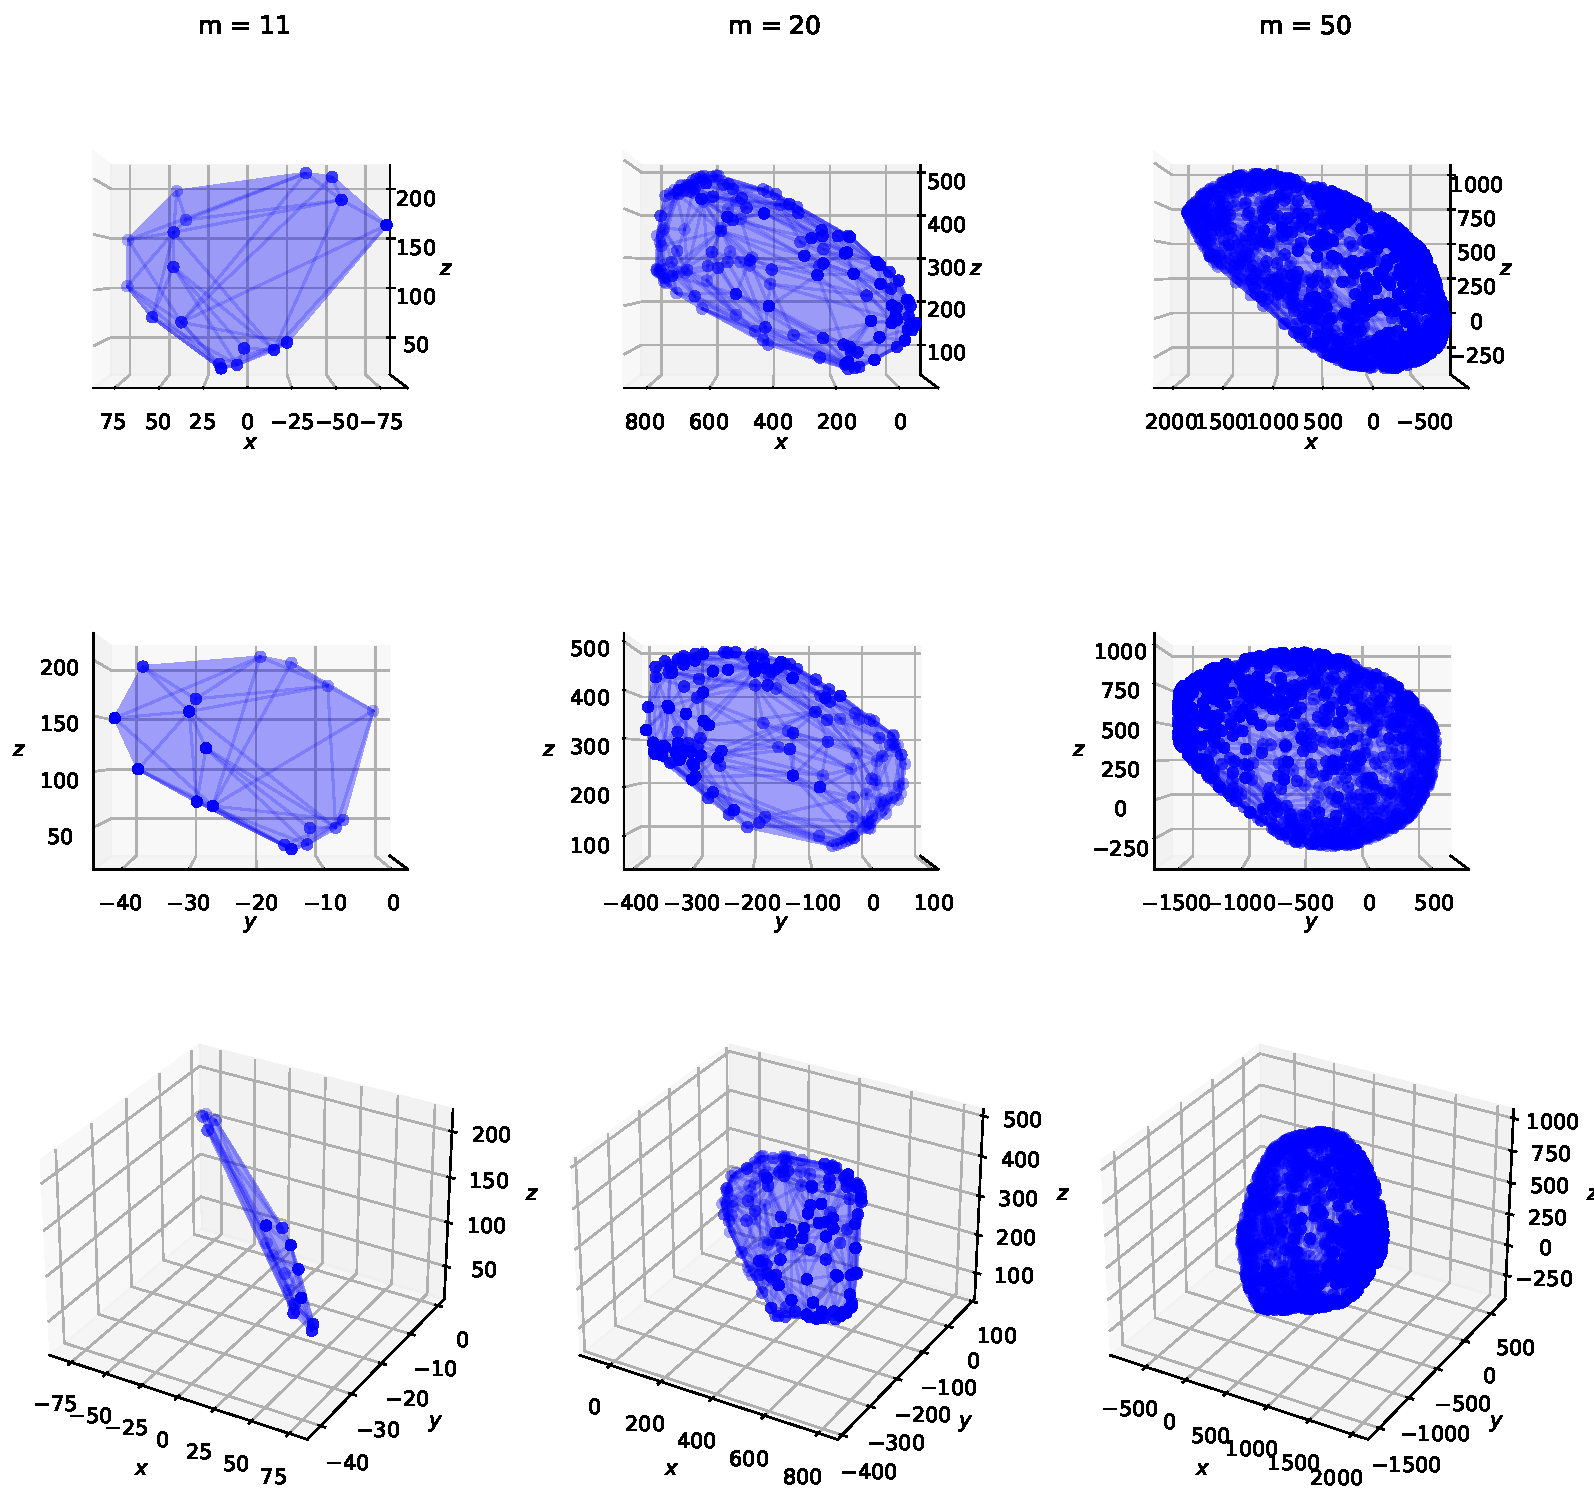
\includegraphics[trim={0 500 0 60},clip, width=0.9\linewidth]{img/chapter_3/zonotopes_looks_like_ellipsoids_2.pdf}
    \end{minipage}
    \begin{minipage}{1\linewidth}
        \centering
        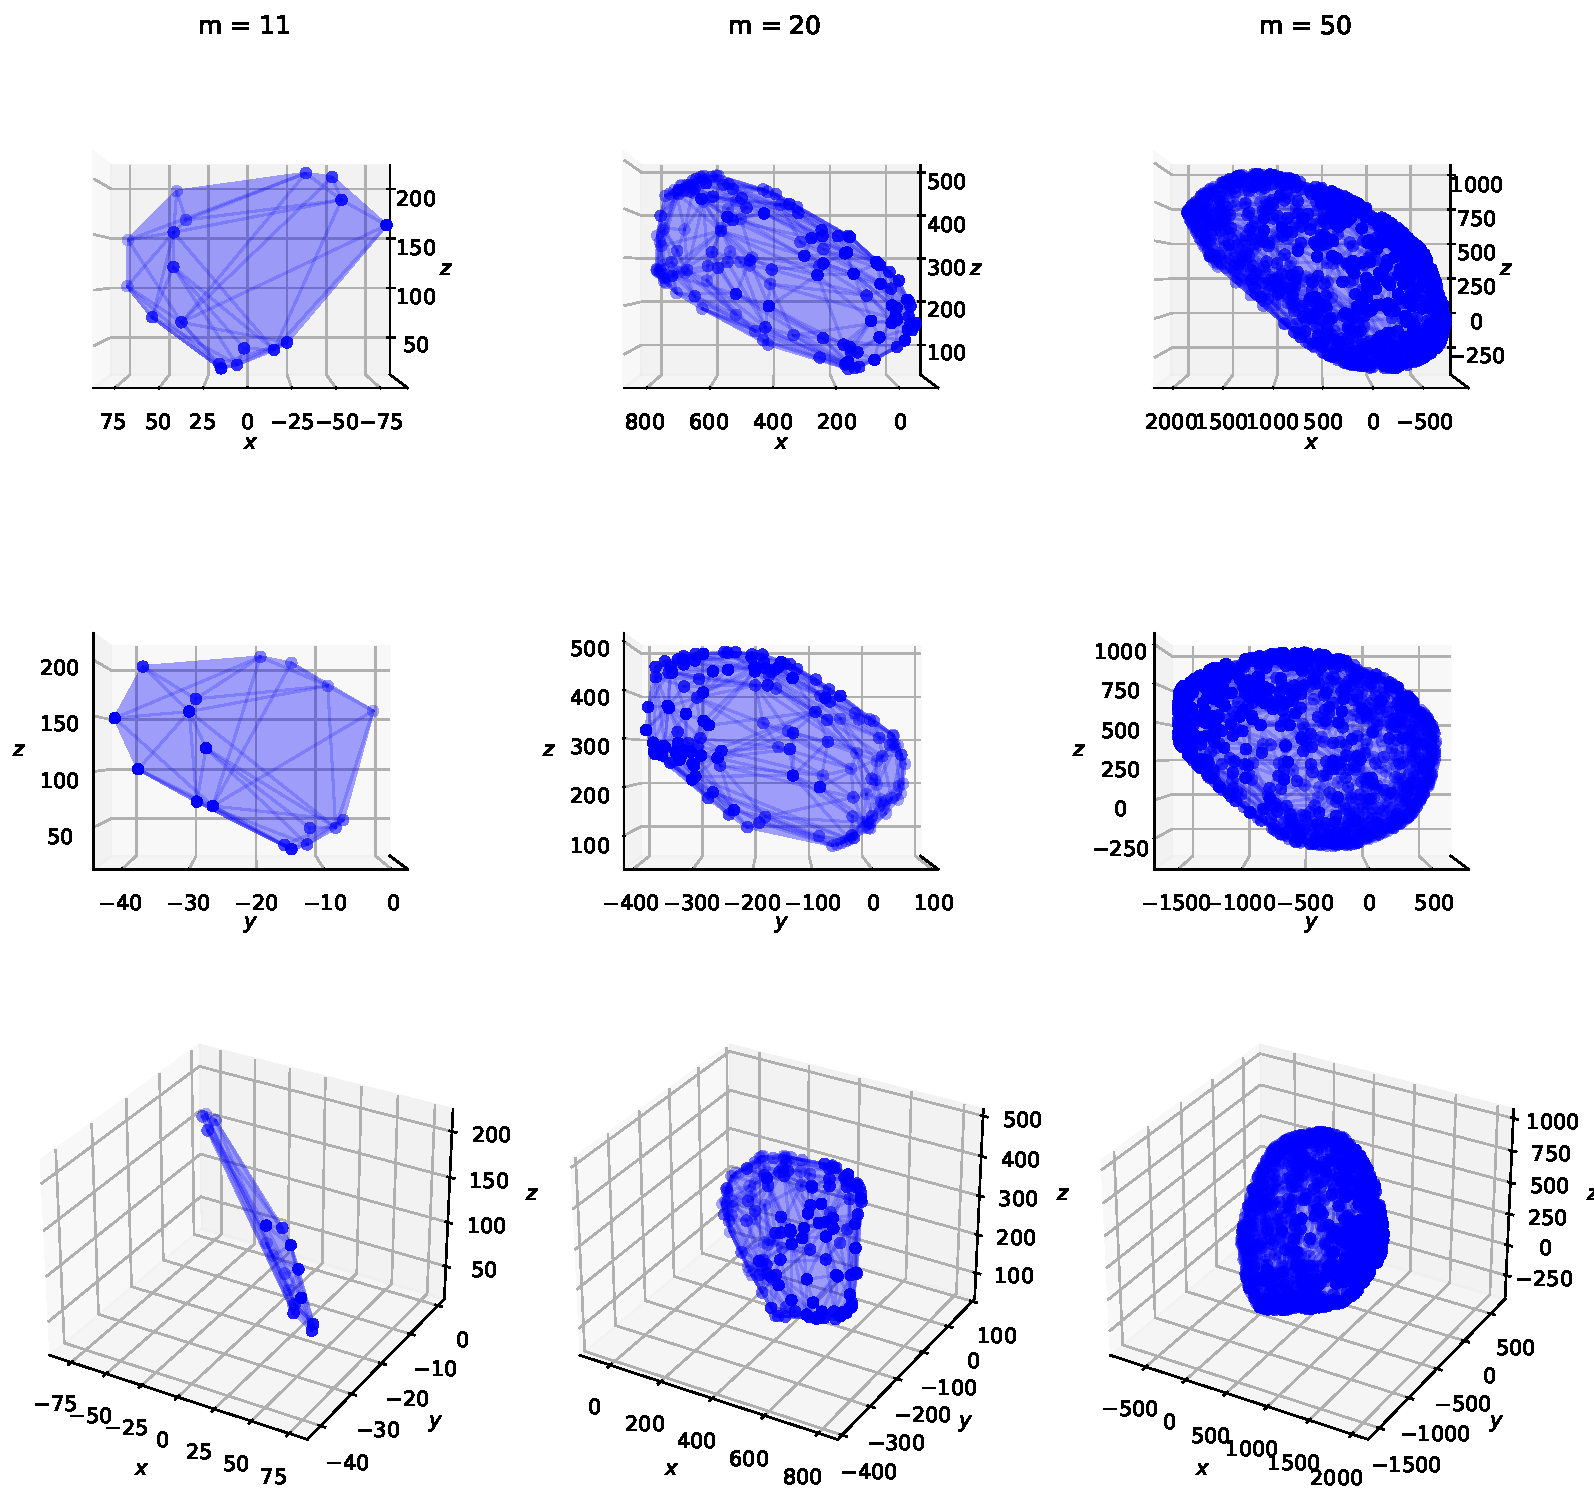
\includegraphics[trim={0 255 0 300},clip, width=0.9\linewidth]{img/chapter_3/zonotopes_looks_like_ellipsoids_2.pdf}
    \end{minipage}
    \begin{minipage}{1\linewidth}
        \centering
        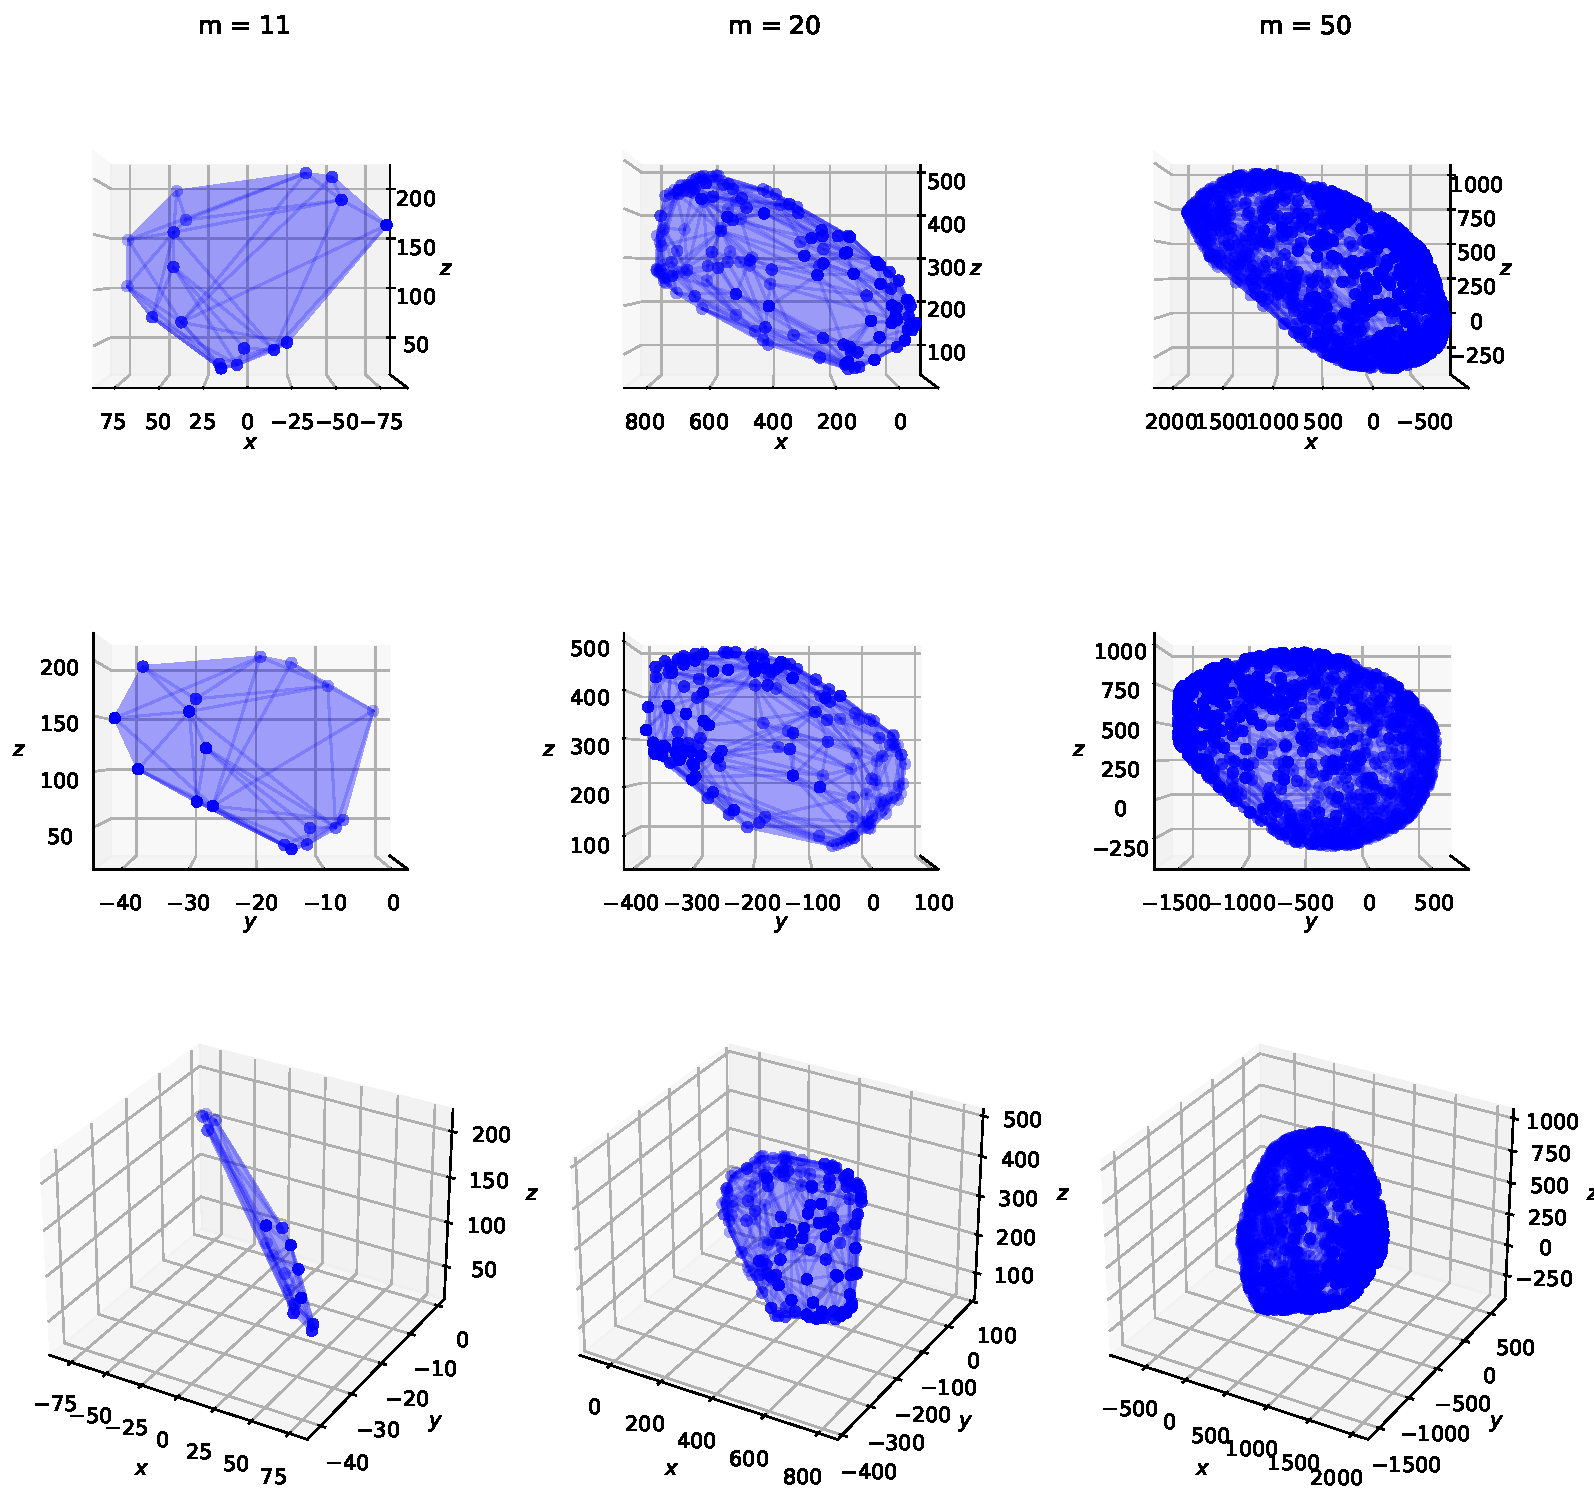
\includegraphics[trim={0 0 0 500},clip, width=0.9\linewidth]{img/chapter_3/zonotopes_looks_like_ellipsoids_2.pdf}
    \end{minipage}
    
    \caption{Each column correspond to a different number of muscles ($m=11$, $20$ and $50$). Each row is a different orientation of the computed force feasible set to better grasp the 3D. Here, the lever arm matrix was considered to describe $7$ degrees-of-freedom over $2$ 3D joints and one pin joint. Each muscle acts on maximally $2$ joints.}
    \label{fig:example_ellipsoidal_zonotope_bijoints}
\end{figure}

This figure shows us how the ellipsoidal shape of a force feasible set can occur. In this example (and actually in almost all cases when $-L^T$ is generated as described), we see that the ellipsoidal shape is qualitatively rather good at $m=50$, which is a lesser bound than expected ($m\geq 68$). We explain this phenomenon by the geometric construction leading to Milman's quotient of subspace theorem \ref{th:milman_quotient_subspace_theorem}. It should be noted that we are observing this ellipsoidal shape by considering a gravity vector, as well as a non-centered tension cube. These two conditions were not explicited in Milman's theorem, even though it was hypothesized.

However, in context we shall never consider muscles acting on \emph{all} joints. There are mono-articular muscles which are acting on only one joint, and bi-articular acting on two joints. In figure \ref{fig:example_ellipsoidal_zonotope_bijoints}, $-L^T$ has been resampled this way: we divide the $7$ rows of $-L^T$ into 3 joints: the first corresponds to the 3 first rows, the second to rows 4 to 6, and the third to the last row (it could represent a pin joint for instance). We will use the term \emph{act} to precise that the values of a column are non-zeros.
The first $15$ muscles (columns) act onto the first joint only (so on the three first rows), the $5$ next on the first and second joint, the $15$ next on the second joint only, the $10$ next on the second and third joint, and the $5$ last muscles act on the third joint. These choices are arbitrary; the core idea is to consider mainly mono- and bi-articular muscles. The results are described in figure \ref{fig:example_ellipsoidal_zonotope_bijoints}, and it can be observed that an ellipsoidal shape is also appearing from $20$ muscles.

\subsection*{Conclusion}

To conclude this section, one of the thesis goal is to understand the shape of the force feasible set. In the litterature, it is often represented under the shape of a polytope or an ellipsoid. This implies that the underlying tension set is modelized in a cube-like manner or a sphere. What we argued is that no matter how the the tension set is modeled, if a sufficiently large amount of muscles are considered then the force and torque feasible sets have a high probability to resemble ellipsoids. This property is due to their geometric constructions.

However, there is a very strong difference in \emph{size} for different tension set models, even though at the end everything resembles an ellipsoid. One way to account for this difference in size would be to compute directly an ellipsoid approximation of the produced force feasible set when using a $\mathcal{T}_{\infty}$ model. 

Let's describe some of these approximations and see how they are computationally not worth. The inner and outer Löwner-John ellipsoids are two ellipsoids commonly used to approximate a convex body. For a $n$-dimensional convex body $C$, its associated inner ellipsoid (or John ellipsoid) refers to the $n$-dimensional ellipsoid of maximal volume inscribed in $C$. The outer ellipsoid (or Löwner ellipsoid), is the circumscribed ellipsoid of minimal volume.
A strong result, initially proven by John, shows that the inner ellipsoid is \emph{unique} to the convex body. Similarly, the outer one is also unique \cite{henkLownerJohnEllipsoids2012}. However, there is one major drawback: as Cerny mentionned in \cite{cernyGoffinAlgorithmZonotopes2012}, Löwner-John ellipsoids can not be found algorithmically in general cases, so that there is a need to approximate them. In context, we shall collect maximal exerted force measurements, which are then considered as point in the Cartesian space.
\begin{itemize}[noitemsep]
    \item The inner ellipsoid is constructed from a set of bounding hyperplanes;
    \item The outer ellipsoid is constructed from a set of points.
\end{itemize}

Constructing them for a set of experimental forces is possible. But trying to fit a musculoskeletal model reproducing the experimental ellipsoid is not tractable: this would mean that the vertices of the torque zonotope should be computed (and transformed into hyperplane inequalities), then the inner or outer ellipsoid can be computed. The combinatorial nature of enumerating these vertices being time-consuming (cf. \ref{chapter:2}), this is not envisageable.

Another drawback is when the tension set $\mathcal{T}$ is derived from a $p$-ball: when projected onto the torque space, except in the cases $p=1,\,2$ or $\infty$, there is no \emph{explicit} description of the surface of the newly created convex body. While a sampling method could be used, if the number of muscles is large, the sampling of the unit $p$-ball would require so much points and the probability that we sample an extremal point of $\mathcal{T}$ projecting onto an extremal point of the torque feasible set is 0.

% \paragraph*{Goffin's ellipsoid \cite{goffinVariableMetricRelaxation1984} adapted=\cite{cernyGoffinAlgorithmZonotopes2012}.}
% We could also consider Gasmann et al. ellipsoid approximations \cite{gasmannScalableZonotopeEllipsoidConversions2020}

Instead of directly computing ellipsoid approximations of a set of points, we shall better understand how the shape and the dimension of the tension set affects the size of the torque feasible set, and thus the force feasible set. The next section, while theoretic at first, offers a computational tool to compute through a simple formula any ellipsoidal approximation of the force feasible set, when a large number of muscles is considered. This formula does not require any points to be computed, hence we remove any combinatorial issues related to enumerating zonotope vertices and it extends to all possible $\mathcal{T}_p$ models.

\section{Accounting for the projected volume problem}
\label{sec:projected_volume_problem}
Our main goal is to show that if a large number of muscles is considered, any choice of a tension set $\mathcal{T}_p$ modelized from a unit $p$-ball results in force feasible sets whose shape are similar and only differ in volume. This section focuses on the volume problem which \emph{naturally} occurs when projecting convex sets onto much lower-dimensional spaces. Subsection \ref{subsec:proj_unit_p_ball} describes the problem through examples, followed by \ref{subsec:projection_constant} which focuses on how this problem occurs. Using a surprisingly non-trivial modern notions in the theory of Banach spaces, called \emph{projection constants}, we will give a strong computational tool to counteract the volume problem and argue about the choice of a $p$-norm.

\subsection{Projection of unit \emph{p}-balls}
\label{subsec:proj_unit_p_ball}
As an introductory example, consider our previous example \ref{fig:example_ellipsoidal_zonotope_bijoints}. Force polytopes were displayed with different scales in order to emphasize their shapeness and not focus on their size. Figure \ref{fig:example_ellipsoidal_zonotope_bijoints_same_scale} shows their sizes according to the same scale.

\begin{figure}[!htb]
    \captionsetup{justification=centering}
    \begin{minipage}{1\linewidth}
        \centering
        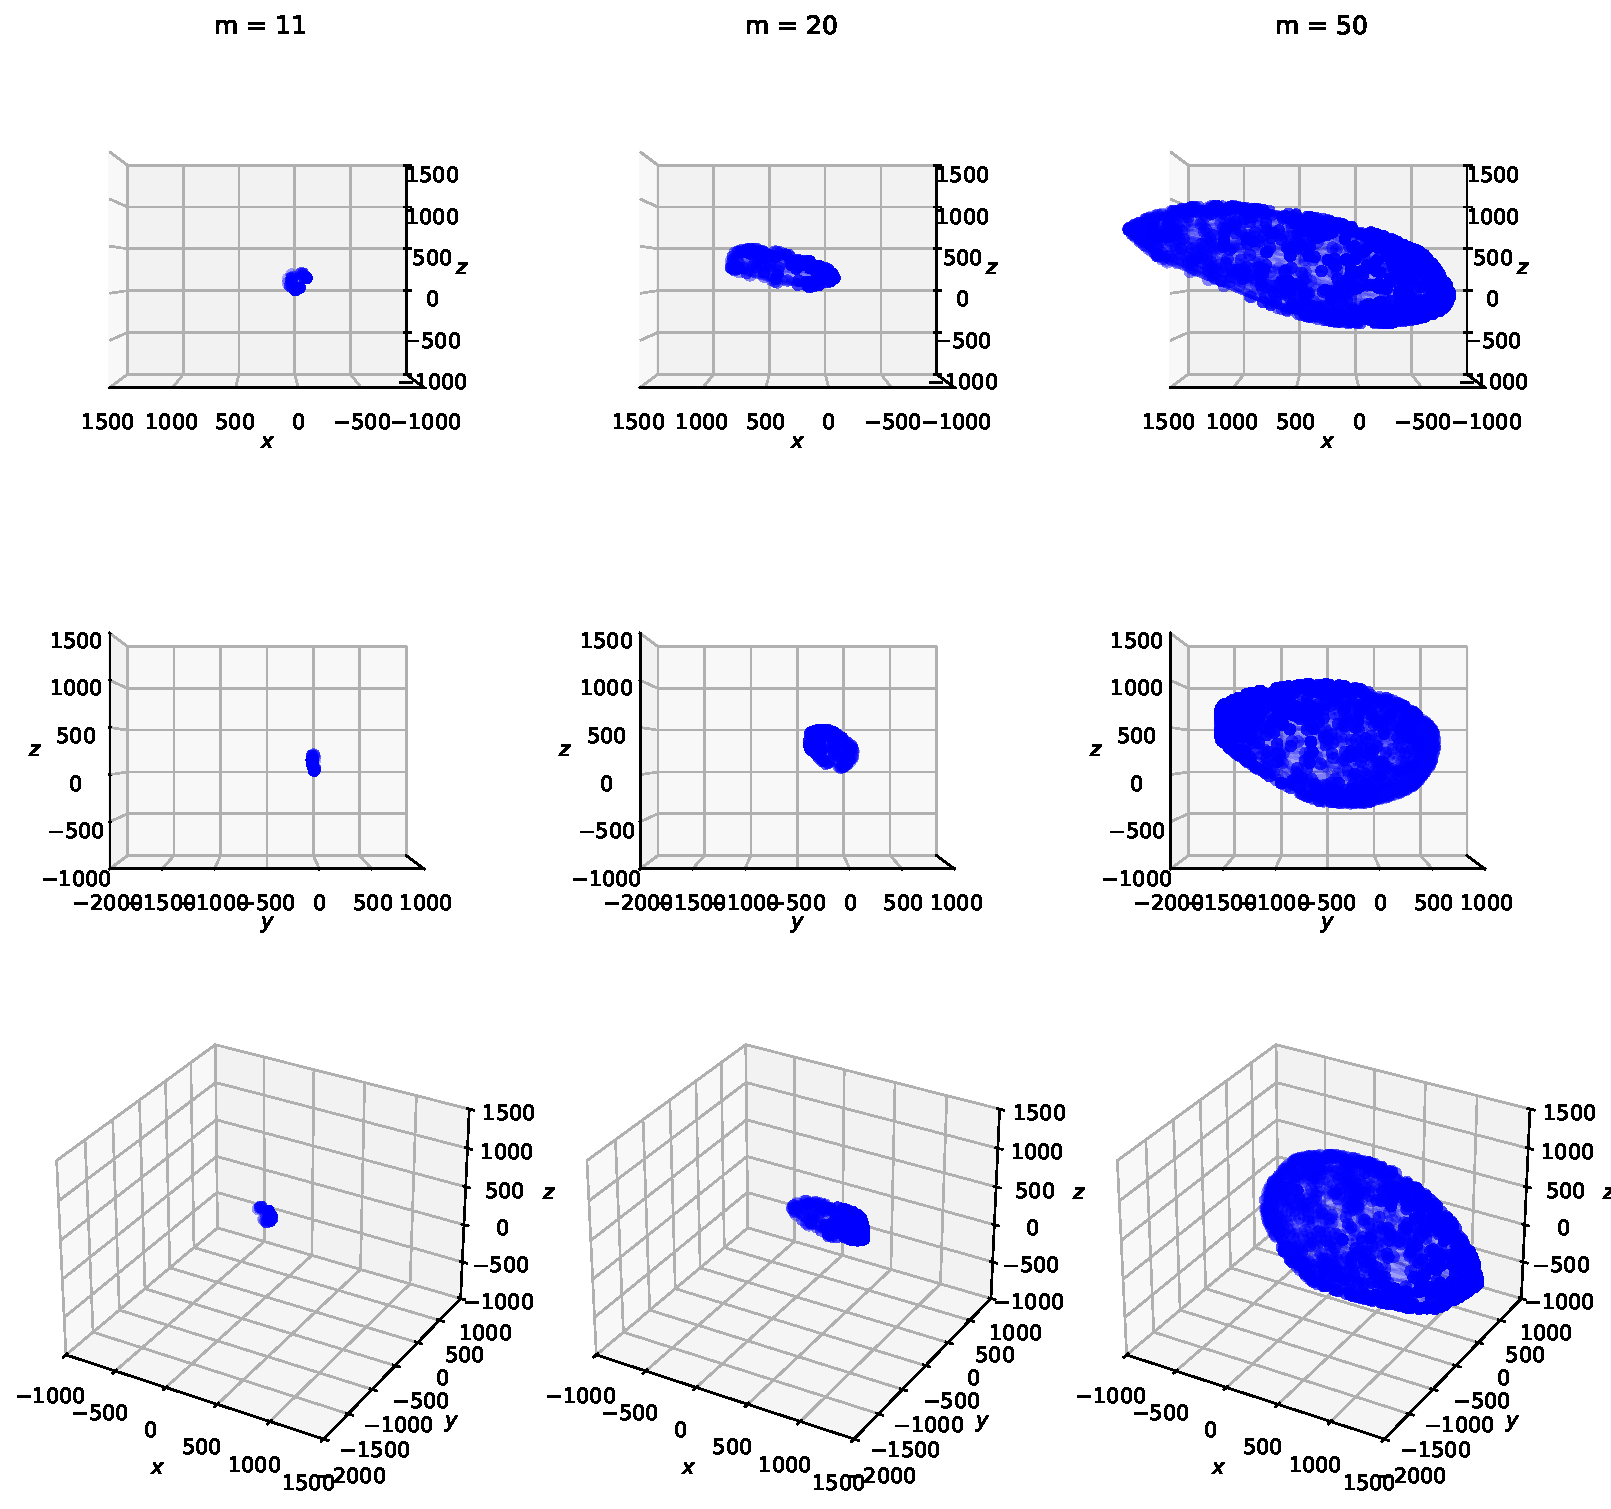
\includegraphics[trim={0 700 0 0},clip, width=0.9\linewidth]{img/chapter_3/zonotopes_looks_like_ellipsoids_2_same_scale.pdf}
    \end{minipage}
    \begin{minipage}{1\linewidth}
        \centering
        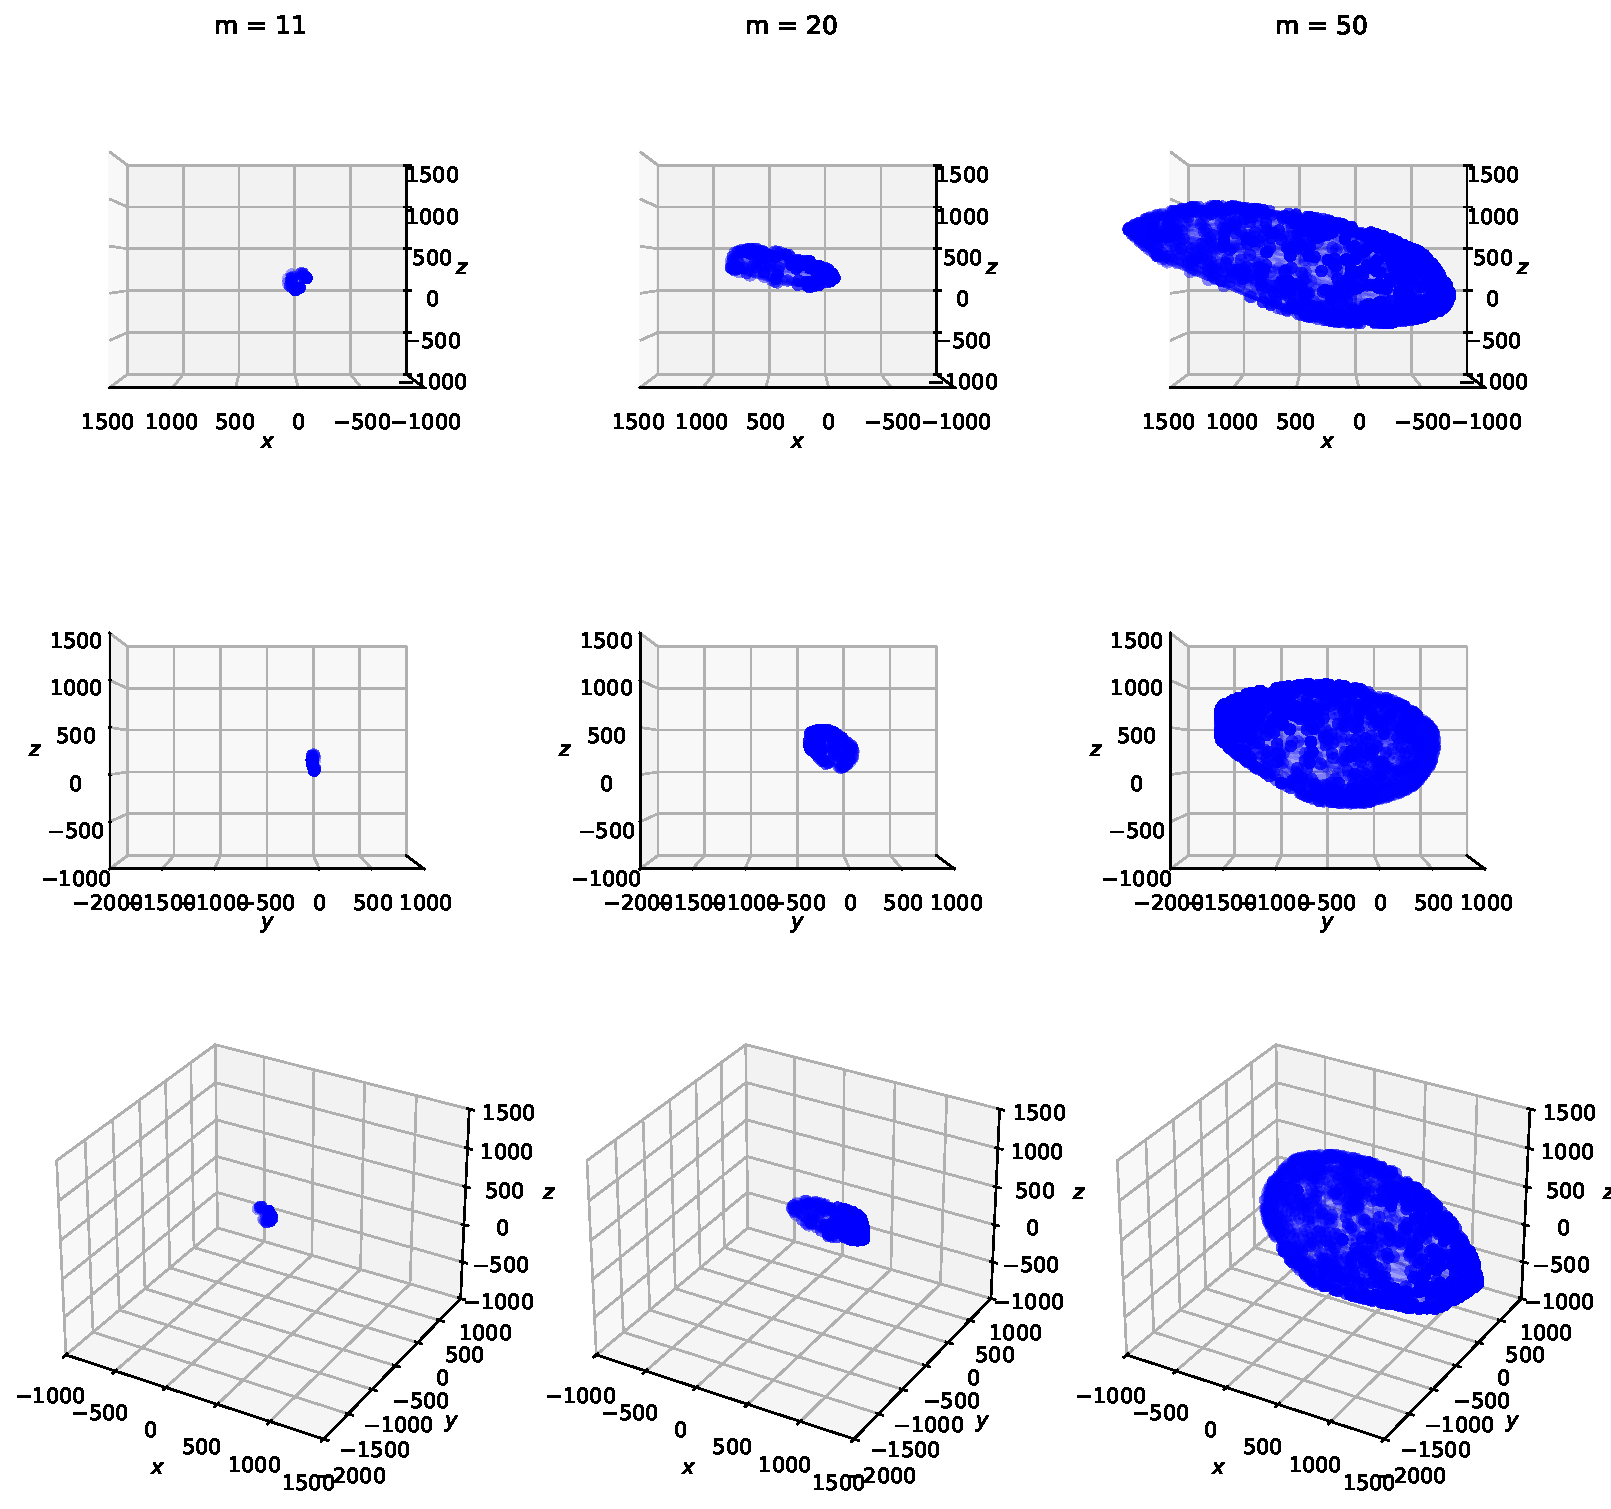
\includegraphics[trim={0 500 0 60},clip, width=0.9\linewidth]{img/chapter_3/zonotopes_looks_like_ellipsoids_2_same_scale.pdf}
    \end{minipage}
    \begin{minipage}{1\linewidth}
        \centering
        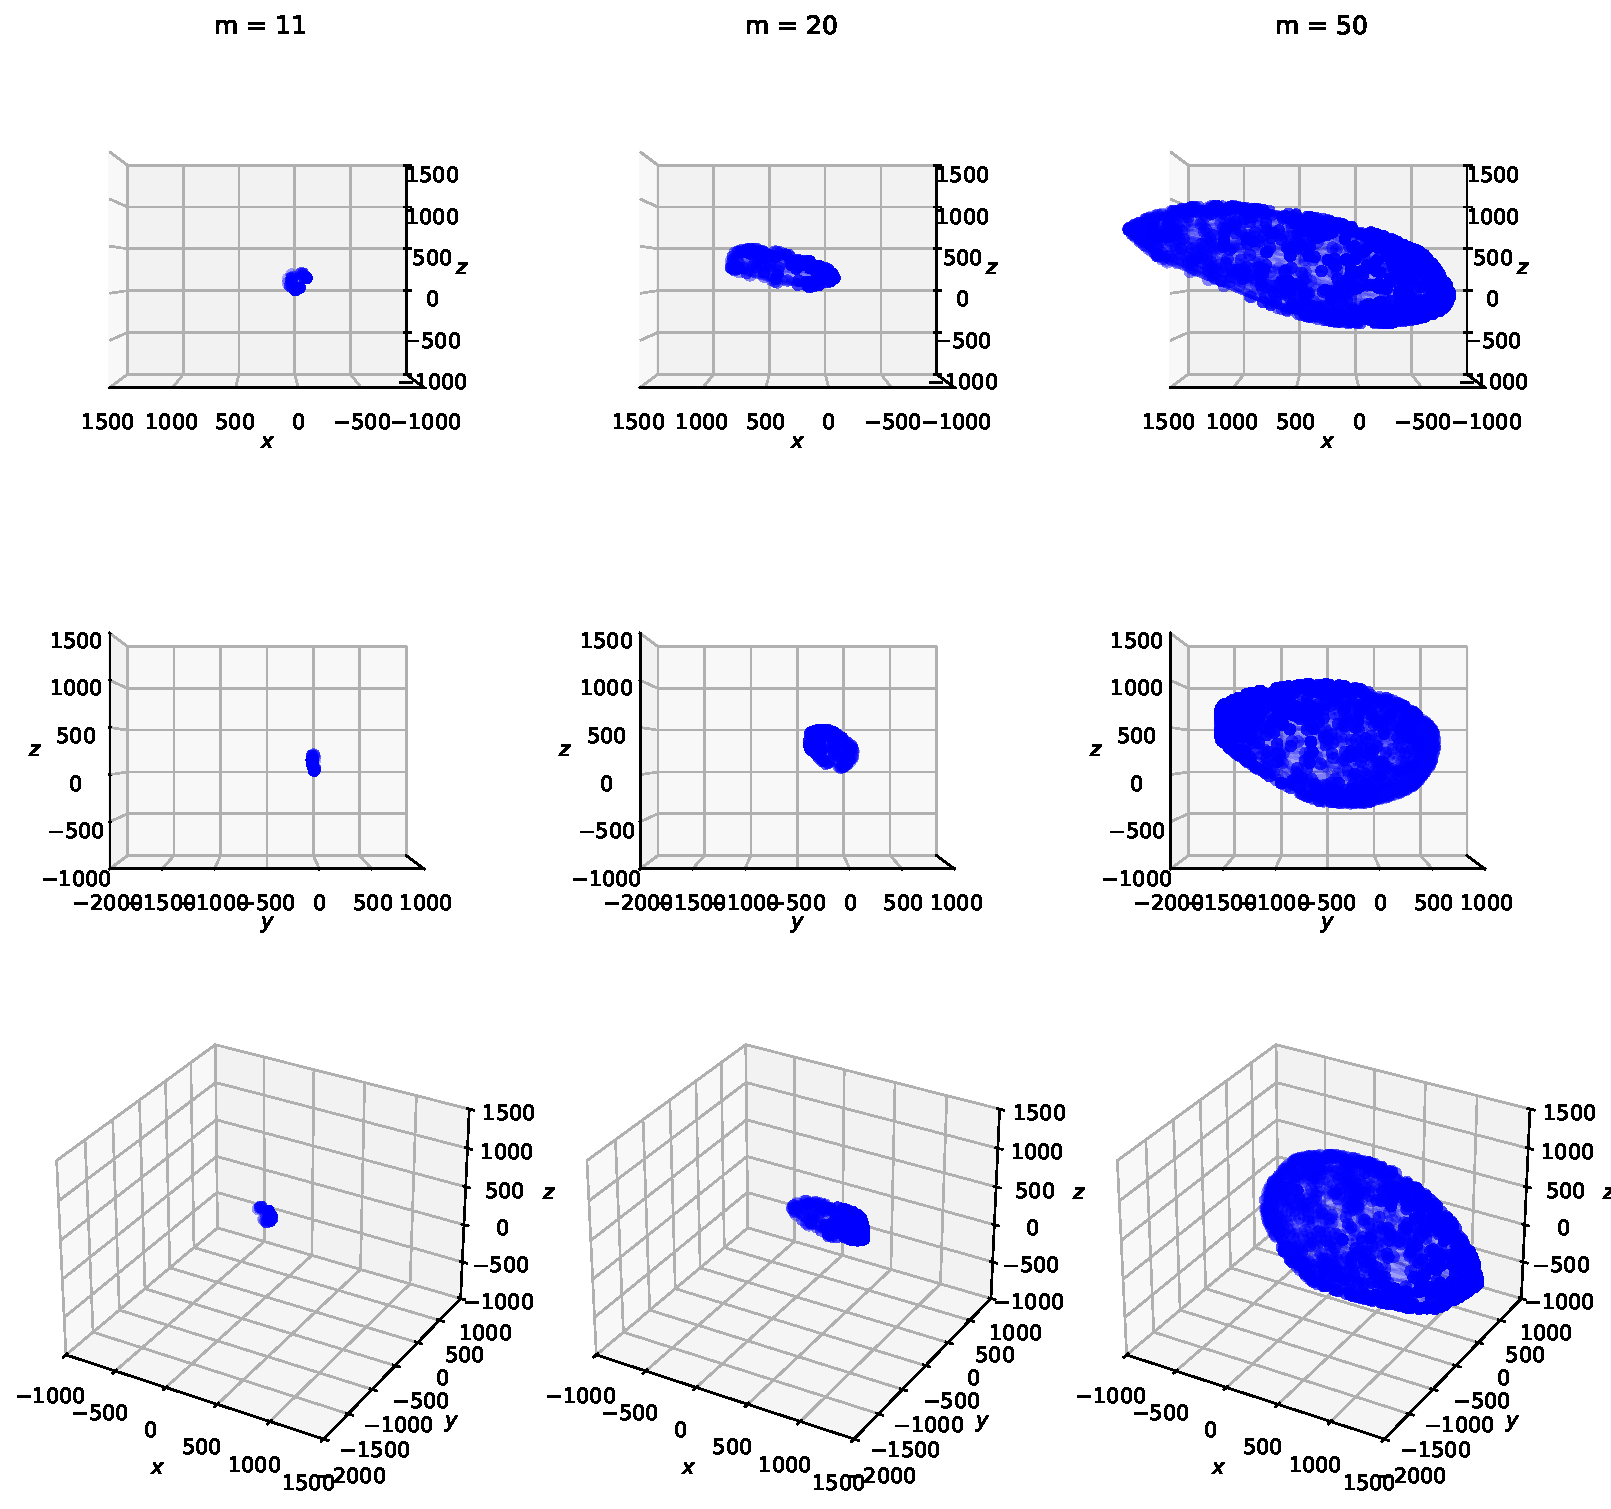
\includegraphics[trim={0 255 0 300},clip, width=0.9\linewidth]{img/chapter_3/zonotopes_looks_like_ellipsoids_2_same_scale.pdf}
    \end{minipage}
    \begin{minipage}{1\linewidth}
        \centering
        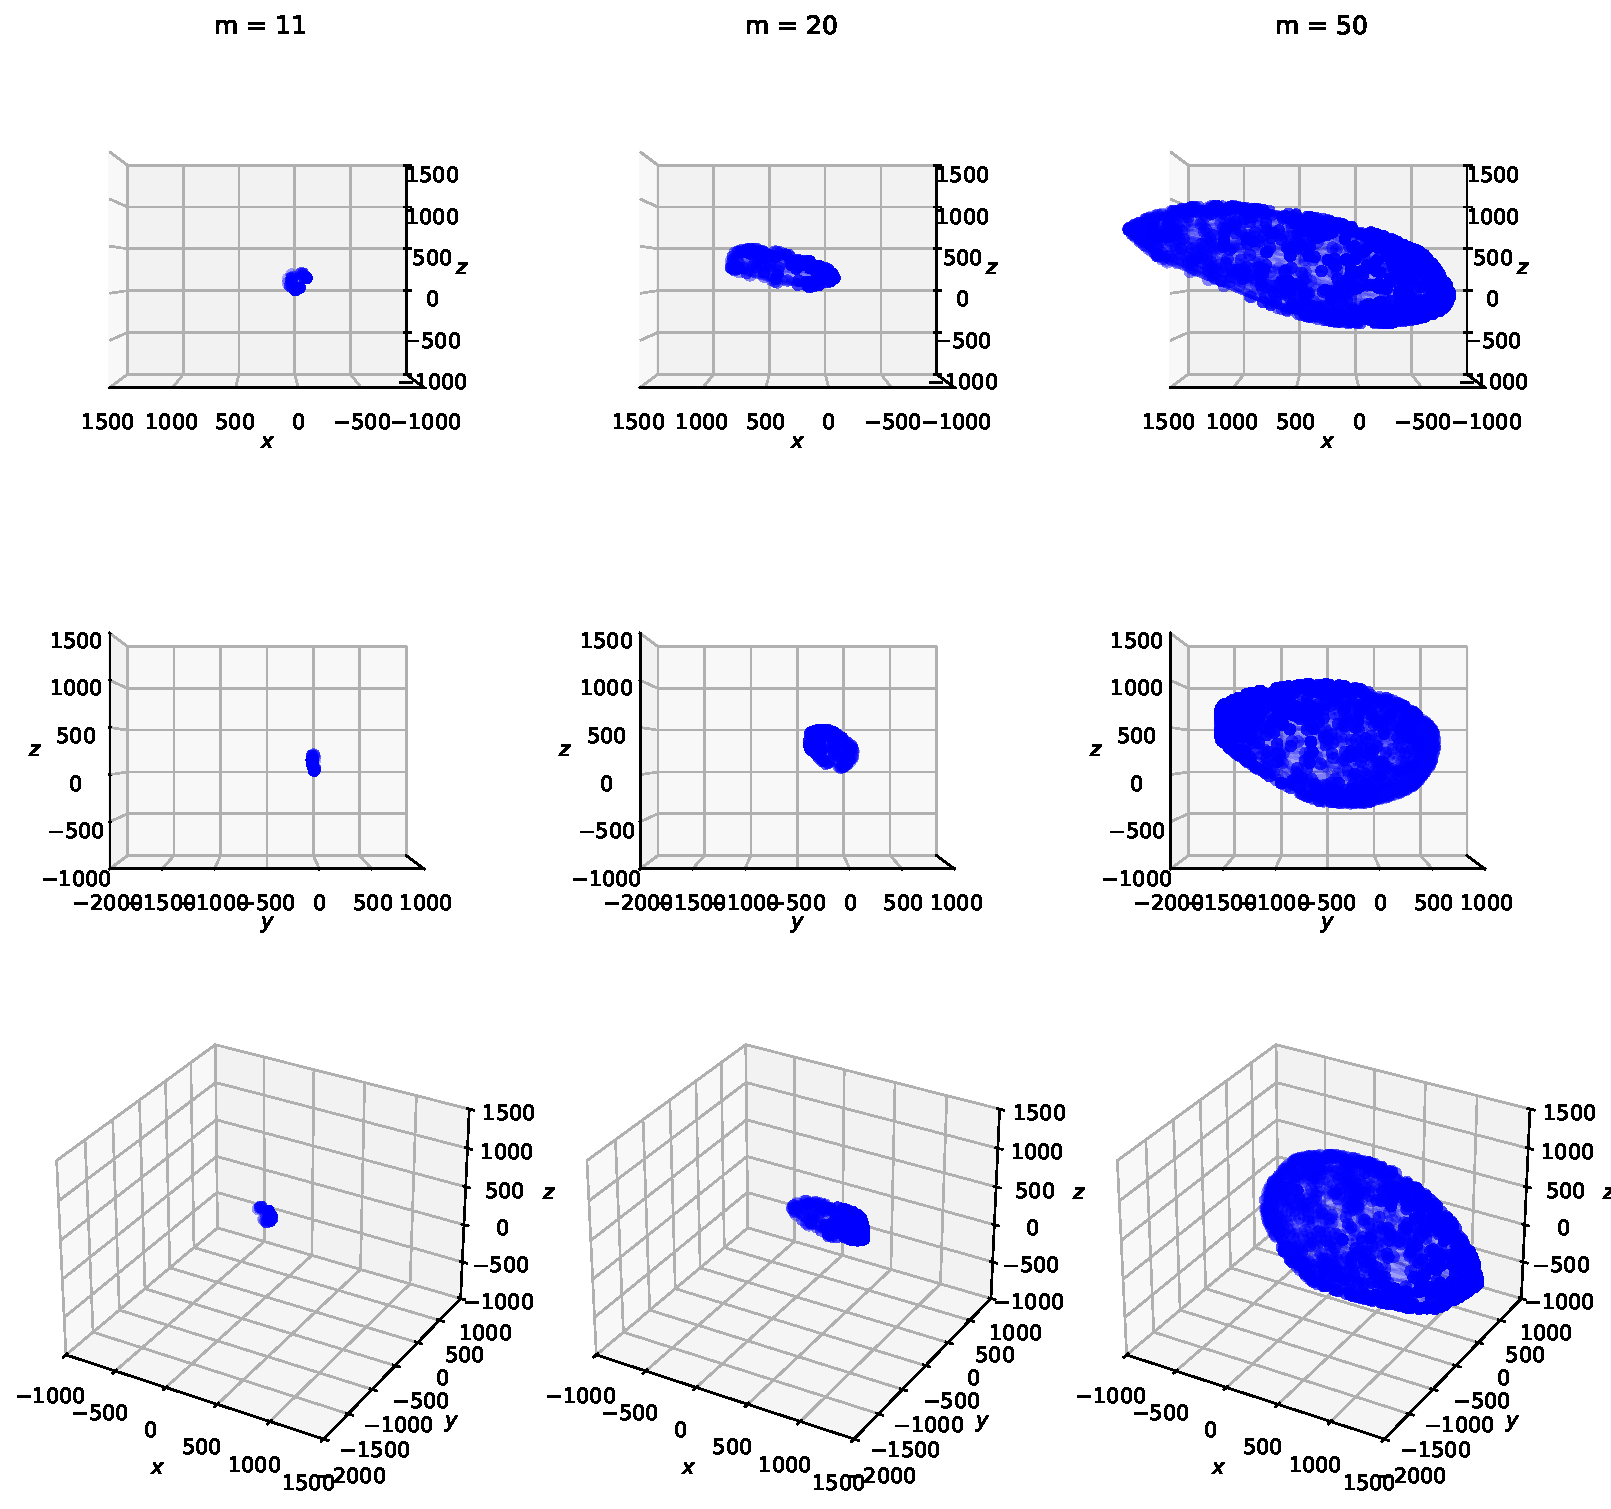
\includegraphics[trim={0 0 0 500},clip, width=0.9\linewidth]{img/chapter_3/zonotopes_looks_like_ellipsoids_2_same_scale.pdf}
    \end{minipage}
    
    \caption{Same example as figure \ref{fig:example_ellipsoidal_zonotope_bijoints} but with the same scale for every force polytope displayed.}
    \label{fig:example_ellipsoidal_zonotope_bijoints_same_scale}
\end{figure}

What should be noticed is that the more muscles are considered, the bigger the produced force feasible set seem to be. Since we used a tension set as a cube, this is explained as a consequence of the Minkowski sum operations involved in projecting a cube to create the torque feasible set as a zonotope. If a sphere was used instead of a cube, it is noticeable that the produced force ellipsoids do not seem to increase their size as rapidly as with a cube model. This is shown in figre \ref{fig:ellipsoid_scale}

\begin{figure}[!htb]
    \captionsetup{justification=centering}
    \begin{minipage}{1\linewidth}
        \centering
        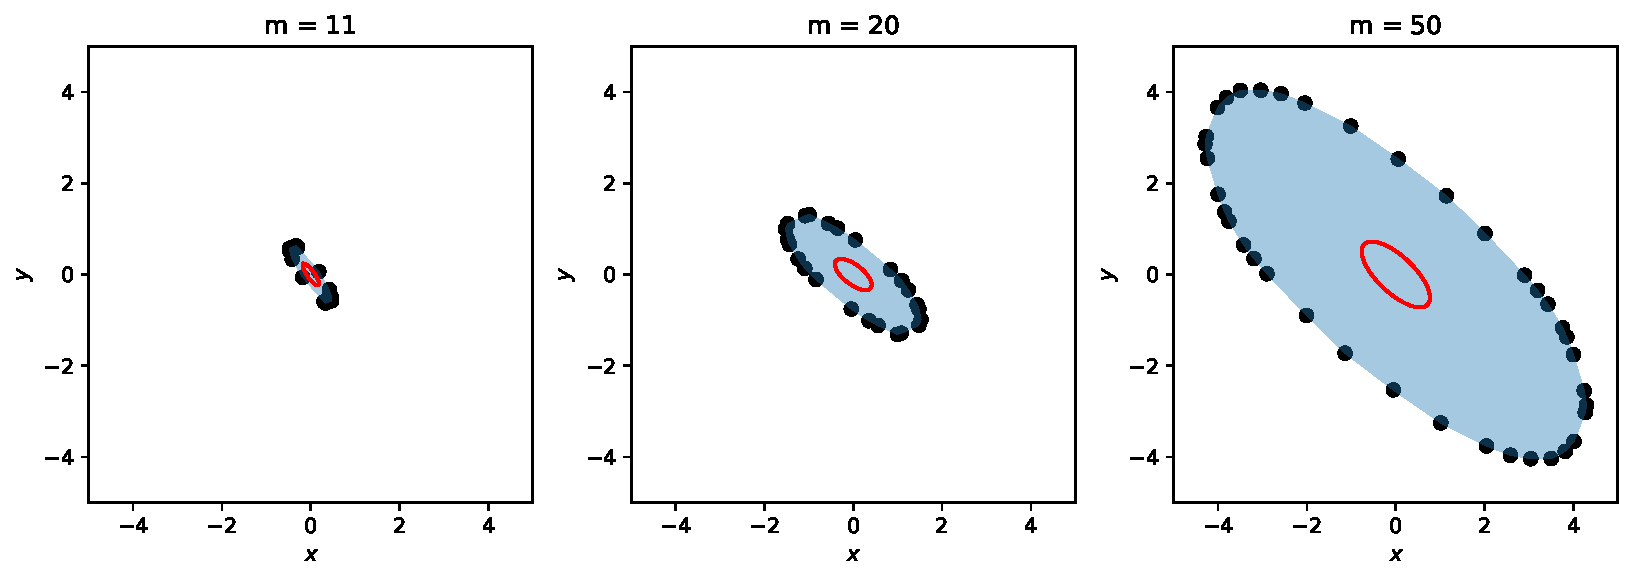
\includegraphics[trim={0 261 0 0},clip, width=0.9\linewidth]{img/chapter_3/ellipsoids_size.pdf}
    \end{minipage}
    \begin{minipage}{1\linewidth}
        \centering
        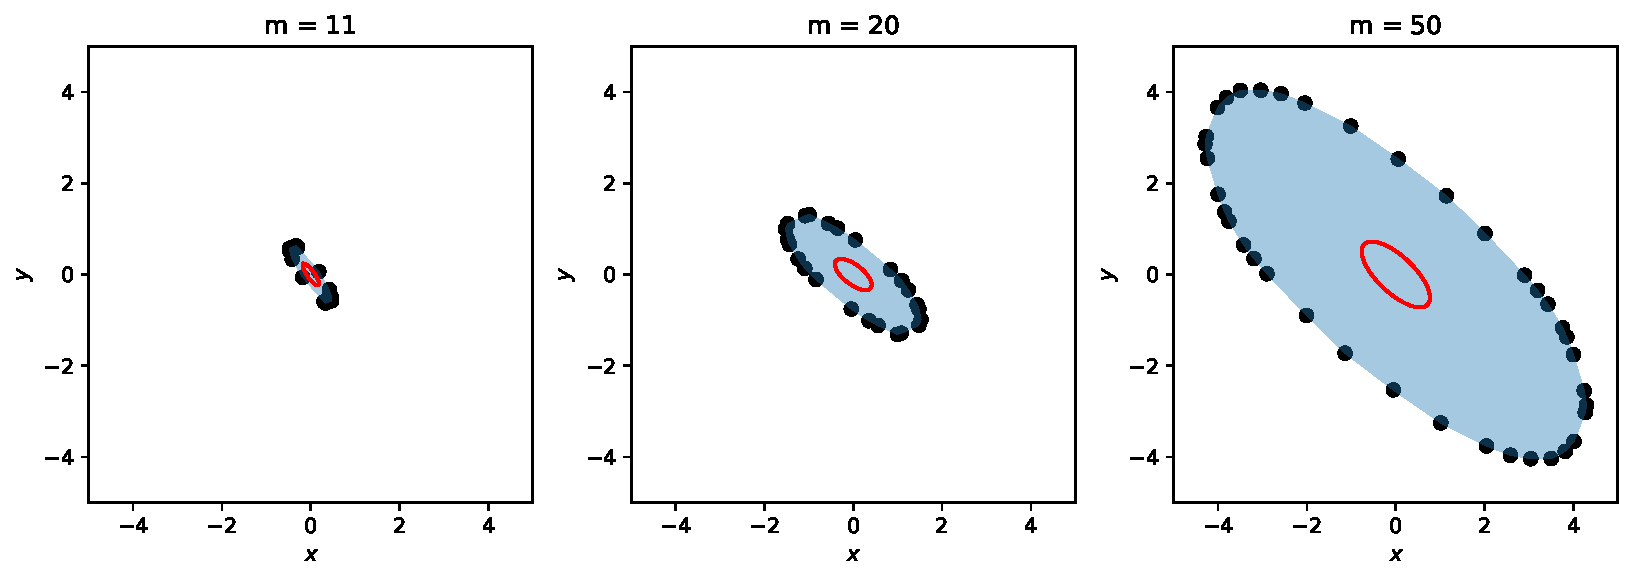
\includegraphics[trim={0 0 0 20},clip, width=0.9\linewidth]{img/chapter_3/ellipsoids_size.pdf}
    \end{minipage}
    
    \caption{Uniformly generated random force feasible sets using a tension set as a sphere (ellipsoids in red) or a cube (polytopes in blue) in $m$ dimension. It seems that the size of the force feasible sets depends on the dimension of the tension set as well as on the choice of its shape.}
    \label{fig:ellipsoid_scale}
\end{figure}

So, how to explain this phenomenon? Since we do want to approximate force polytopes by ellipsoids, we have to increase the size of the given ellipsoid by some coefficient which seem to depend on the tension set dimension. Since the size of a vector leads to the notion of the size of an object, there is necessarily a link to the notion of volume.
Consider in $\IRm$ the unit $2$-ball $\mathcal{B}_2^m$ and $\infty$-ball $\mathcal{B}_{\infty}^m$, \emph{i.e.} respectively an Euclidean ball of radius $1$ and a hypercube of edge length $2$. For $n < m$, consider also a surjective linear map $\psi\colon \IRm\rightarrow \IRn$ of rank $n$ to represent the linear projection from the tension space to the torque space.

For real Banach spaces, John's theorem \cite{johnExtremumProblemsWithInequalities1948} states that $m^{-1/2}\mathcal{B}_{\infty}^m \subset \mathcal{B}_2^m \subset \mathcal{B}_{\infty}^m$ , where $m^{-1/2}\mathcal{B}_{\infty}^m$ denotes the $\infty$-ball with radius $m^{-1/2}$. Since a linear (or affine) map preserves containment, we also have $m^{-1/2}\psi(\mathcal{B}_{\infty}^m) \subset \psi(\mathcal{B}_2^m) \subset \psi(\mathcal{B}_{\infty}^m)$. In other words, the sphere in $\IRm$ can be encapsulated by a cube and the reverse too. 
To ensure our force ellipsoids are rougly the same size as our force polytopes, it was first thought that we could increase the tension set sphere radius to match its volume to the cube volume. In this case, the ratio between volumes of the two tension sets is $1$. To compute the radius of a sphere whose volume equals the volume of the cube, note $V_2^m(R)$ the volume of the $m$-dimensional Euclidean ball of radius $R$. We have
\begin{align}
\label{formula_volume_nsphere}
    V_2^m(R) = \frac{\pi^{m/2}}{\Gamma\left(\frac{m}{2} + 1\right)}R^m
\end{align}
where $\Gamma$ denotes the Euler gamma function, which is an extension of the factorial function to positive real number since $\Gamma(n)=(n-1)!$ if $n$ is a strictly positive integer.

Since the volume $V_p^m(R)$ of a $m$-cube of edge length $2R$ is given by $V_{\infty}^m(R) = (2R)^m$, we can ensure that our $2$-ball has a radius $R'$ of 
\begin{align}
\label{formula:cube_sphere_same_radius}
R' = \left(\frac{\Gamma\left(\frac{m}{2} + 1\right)}{\pi^{m/2}}V_{\infty}^m(1)\right)^{1/m} = \frac{2}{\sqrt{\pi}}\Gamma\left(\frac{m}{2} + 1\right)^{1/m}
\end{align}
and consequently both balls have the same volume in $\IRm$ \emph{i.e.} $V_2^m(R') = V_{\infty}^m(1)$.

However, the ratio between the volumes is not necessarily preserved under a linear map, as seen in figure \ref{fig:ellipsoid_scale_same_volume}.

\begin{figure}[!htb]
    \captionsetup{justification=centering}
        \centering
        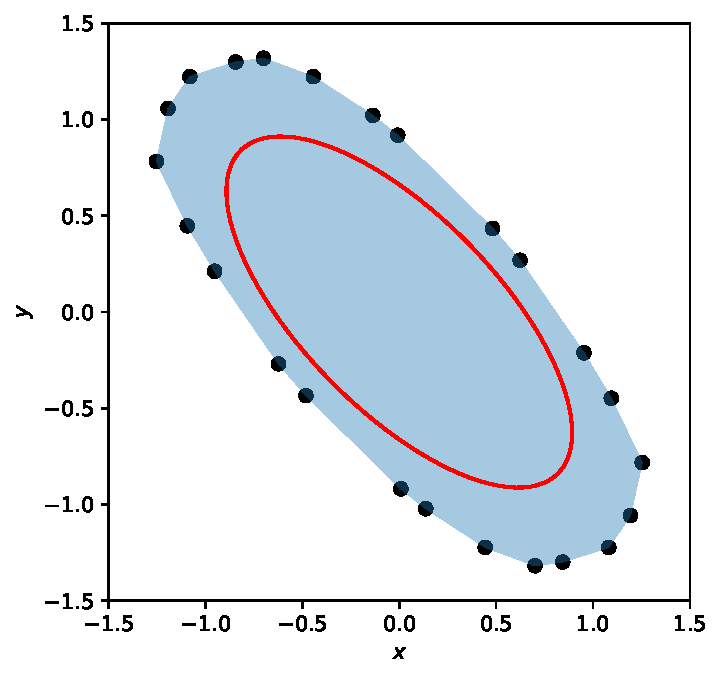
\includegraphics[trim={0 0 0 0},clip, width=0.5\linewidth]{img/chapter_3/myIma4_projection_cube_sphere_same_volume.pdf}    
    \caption{The force polytope (in blue) is produced from a $20$-dimensional unit cube of edge length $2$ of volume $1048576$ N$^{20}$ randomly projected over a $7$-dimensional space then intersected with a random plane. Under the same projection-intersection, the force ellipsoid (in red) is produced from a sphere in $\mathbb{R}^{20}$ of radius $\frac{2}{\sqrt{\pi}}\Gamma\left(\frac{20}{2}+1\right)^{1/20}\sim 2.4012$, ensuring a volume equals to the cube's. This figure shows that \emph{clearly} the volumes are not kept under the projection-then-intersection operation.}
    \label{fig:ellipsoid_scale_same_volume}
\end{figure}

Through this example, we showed that the \emph{shape} of the tension set has an influence on the force feasible set volume. It must be kept in mind that volume is not a \emph{linear} notion, so it does not concentrate in the same way everywhere in a space. Formula \ref{formula:cube_sphere_same_radius} hints that the volume of the cube is mainly concentrated around its corners, since if it had no corners (as the sphere), it would have a decreasing volume over dimensions.

However, we must be careful about generalization: the volume of a measurable set (\emph{i.e.} a set in which the notion of measure/volume makes sense) does not rely entirely on its shape. It is also determined relatively to an arbitrarily chosen object which is defined to be of volume $1$. This object is the $m$-cube of edge length exactly $1$, which means that we can always say if another measurable set \emph{takes more place or not} compared to the unit cube. More formally, the usual notion of volume is called the Lebesgue measure. While very handy, this definition induces a major problem: when transforming an object, the domain space and the codomain space (or the arrival space) do not share the same unit cube, so the way of measuring the transformed object is entirely different \emph{i.e.} the notion of volumes in not directly comparable between $\IRm$ and $\IRn$. Interestingly, the determinant of an application can be seen as a way to describe how the transformation of the notion of measurement between two spaces (the domain and codomain) would fail to make sense.

A practical workaround is to, instead of considering both $\IRm$ and $\IRn$ as two different entities, consider them as subsets of a larger ambiant space in which a unique notion of volume is assumed. But these spaces can be equipped with various metrics (describable notably by $p$-norms), so it must be taken into account as well in order to understand how volume \emph{transit} between these two different normed spaces. This is the goal of the next paragraphs, which explain this workaround and how to use it to create an easily computable novel ellipsoidal approximation of a projected unit $p$-ball.

\subsection{Leveraging the projected volume via the projection constant}
\label{subsec:projection_constant}
\emph{Projection constants} are a fairly recent approach (mathematically-wise) in the theory of Banach spaces, whose first appearance can be found in Murray's paper from 1937 \cite{murrayCOMPLEMENTARYMANIFOLDSPRO}. They are still a subject of interest in our current days \cite{donohoCountingFacesRandomlyProjected2010}, \cite{foucartMaximalRelativeProjection2017}, \cite{bassoComputationMaximalProjection2019}, \cite{defantProjectionConstantsSpaces2022}. Their goals are to quantify the worst-case scenario of a unit ball deformation. Translated in our context, they describe how large the radius of a sphere should be to behave volume-wise as if it was a cube. In a more general manner, they compute the radius of any $p$-ball to behave as another $q$-ball. 

Biomechanically speaking, we will use them as a tool to express an ellipsoid approximation of a tension set whose activation interactions are modeled using a $p$-ball. So, if the working biomechanician decides to enable a very high-level of interactions (\emph{i.e.} activations follow a cube-like shape), then there suffices to compute the force feasible set as an ellipsoid (using a sphere for the tension set) and multiply its radius by the projection constant related to the cube. All other levels of interaction correspond to different shapes described a choice of $p$ in between $2$ and $\infty$.

A few novel notions should be defined to compute these projection constants.

\paragraph*{Isometric embedding.} Let $X$ and $Y$ be Banach spaces. The operator $I\,\colon X\rightarrow Y$ is an \emph{isometric embedding} of $X$ if $I$ is injective, $I(X)$ is a subspace of $Y$ and $I(X)$ is isometric to $X$. The notion of isometric embedding has the sole purpose of describing some space $X$ in a larger dimensional space.

\paragraph*{Projections.} For $X$ a subspace of $Y$, a \emph{projection} $P\,\colon Y\rightarrow X$ is an operator such that $P(x) = x$ for all $x\in X$.

\paragraph*{Projection constant.} For $X\subset Y$ subspace, the \emph{relative projection constant of $X$ in $Y$}, noted $\lambda(X,Y)$, is defined as
$$\lambda(X,Y) = \inf\left\{\|P\|_{op} \mid \text{$P\,\colon Y\rightarrow X$ is a projection} \right\}$$
Projection constants have consequences in approximation theory, as recalled by Defant et al. in \cite{defantProjectionConstantsSpaces2022} stating that for a projection $P\,\colon Y\rightarrow X$ and for all $y\in Y$, the error $\|y-P(y)\|_Y$ satisfies the following
$$\|y-P(y)\|_Y \leq (1 + \|P\|_{op})d(y,X)$$
where $d(y,X) = \inf_{y\in Y}\left\{\|y-x\|_Y \mid x\in X\right\}$. 
To approximate $X$ by $Y$, or in other words, approximate the unit ball of $X$ by the ball of $Y$ (or reversely), the operator norm $\|P\|_{op}$ should be the smallest possible. This happens when $\|P\|_{op} = \lambda(X,Y)$.

So we shall concentrate on the worst scenario possible \emph{i.e.} the highest value of $\|P\|_{op}$ which, in a sense, describes how much can the vectors of unit ball of $Y$ be dilated when projected on $X$. This is called the \emph{(absolute) projection constant} of $X$, noted $\lambda(X)$ and defined as 
$$\lambda(X) = \sup\lambda(I(X),Y)$$
where the supremum is taken over all Banach space $Y$ containing $X$, and over all isometric embeddings $I\,\colon X\rightarrow Y$. In other words, the unit ball of $X$ is described from a higher-dimensional point of view ($Y$) and we compute how elements of the unit ball of $Y$ can deform at best regarding how far they are from the ball of $X$, and this process is repeated over all possible higher-dimensional $Y$ to retrieve the worst case deformation value. 

Another very useful result in the Banach space theory tells us that if $X$ is finite-dimensional, then $X$ can be isometrically embedded into a finite-dimensional $Y$ equipped with the $\infty$-norm. Since it works for \emph{any} such $X$, finding $\lambda(X)$ is equivalent to finding the norm of a minimal projection from a finite-dimensional space equipped with the $\infty$-norm. This result is recalled in \cite{defantProjectionConstantsSpaces2022}.

While understandably not trivial to formulate and represent, we shall clearly see this $\lambda$ value as a metric stating how large the size of some projected $p$-ball can be compared to another unit $p$-ball. 
% Once this metric is retrieved, we shall take this second $p$-ball and multiply it by the computed value to obtain a worst-case approximation (in size) of the first projected $p$-ball. In practice in the context of choosing a modeling for the tension set $\mathcal{T}$, it tells us that whatever the choice of $p$ for $\mathcal{T}_p$, we can adapt the size of the torque feasible set (in volume) afterwards to fit another chosen $p$. Let's recall that the choice of $p$ can be seen as how the working biomechanician or robotician would choose to model the interactions between muscle tensions.

Now, since there are an infinite amound of projections, of isometric embeddings and of higher-dimensional Banach spaces, the essential part of the projection constants theory is to compute their bounds or exact values for various cases, and as of recently, some projection constants are still a strong subject of interest \cite{defantProjectionConstantsSpaces2022}, \cite{deregowskaSimpleProofGrunbaum2023}, \cite{deregowskaValueFifthMaximal2022}, \cite{chalmersMINIMALPROJECTIONSABSOLUTEPROJECTION}, \cite{bassoComputationMaximalProjection2019}, \cite{foucartMaximalRelativeProjection2017}.
We are particularly interested in the cases of $\ell_p^n$ spaces, which denote the spaces of $\IRn$ equipped with the $p$-norm $\|\cdot\|_p$. We recall that they are assimilated to various shapes of the tension set. The following theorem encapsulates almost a century of results over projection constants for $\ell_p^n$ spaces:

\begin{theorembox}{Projection constant of $\ell_p^n$ spaces}{proj_constant_lp_spaces}
    Let $\ell_p^n$ be the finite-dimensional normed space $\IRn$ equipped with the $p$-norm $\|\cdot\|_p$ defined for all $x\in \ell_n^p$ as $\|x\|_p=\left(\sum_{i=1}^n \vert x\vert^p\right)^{1/p}$. Denote by $\lambda(\ell_p^n)$ the projection constant of $\ell_p^n$. Then we have

    \vspace{5mm}

    \begin{itemize}
        \item {\underline{For $p=2$:}
        $$\lambda(\ell_2^n) = \frac{2}{\sqrt{\pi}}\frac{\Gamma(\frac{n}{2} + 1)}{\Gamma(\frac{n}{2} + \frac{1}{2})}$$
    where $\Gamma$ is the Euler gamma function defined for all $z\in \mathbb{C}$ with strictly positive real part as $\Gamma(z)=\int_0^{+\infty}t^{z-1}e^{-t}\,dt$.}
        \item{\vspace{5mm}\underline{For $p=1$:}
    $$\lambda(\ell_1^n) = \begin{cases} 
        \lambda(\ell_2^{n-1}), & \text{if $n$ is even} \\
        \lambda(\ell_2^n), & \text{if $n$ is odd}
     \end{cases}$$
        }
        \item{
            \vspace{5mm}
            \underline{For $2<p<\infty$}:
            $$\lambda(\ell_1^n) = O(n^{\frac{1}{p}})$$
            where $O$ is a Big O notation describing an asymptotic growth.
        }
        \item{
            \vspace{5mm}
            \underline{For $1<p<2$}:
            $$\lambda(\ell_p^n) \approx \sqrt{\frac{2n}{\pi}}\quad \text{as $n\rightarrow +\infty$}$$
        }
    \end{itemize}
\end{theorembox}
\begin{proof}
    The cases $p=1$ and $p=2$ have been proven by Grünbaum in 1960 in \cite{grunbaumProjectionConstants1960}.
    The asymptotic bound for the cases $2<p<\infty$ has been proven by Garling and Gordon \cite{gordonProjectionMacphailConstants1968}, \cite{garlingRelationsConstantsAssociated1971}.
    The approximation given in the case $1<p<2$ has been decribed by König et al. in \cite{konigProjectionConstantsSymmetric1999}.
\end{proof}
It should be noted that the values given in this theorem apply only for a \emph{real} normed space. For the complex version, the reader is invited to find these adapted projection constant values in Defant et al. 2022's paper \cite{defantProjectionConstantsSpaces2022}.

We shall conclude this subsection by figure \ref{fig:example_proj_constant_applied}. It is an example of an approximation of a zonotope generated from a large number of generators by an ellipsoid computed using the projection constant $\lambda(\ell_2^{m})$ for $m=11$, $20$ and $50$. This is equivalent to say that we used an approximation of the $\mathcal{T}_{\infty}$ model by a $\mathcal{T}_2$ model using only a dilating factor given by $\lambda(\ell_2^{m})$. 


\begin{figure}[!htb]
    \captionsetup{justification=centering}
    \begin{minipage}{1\linewidth}
        \centering
        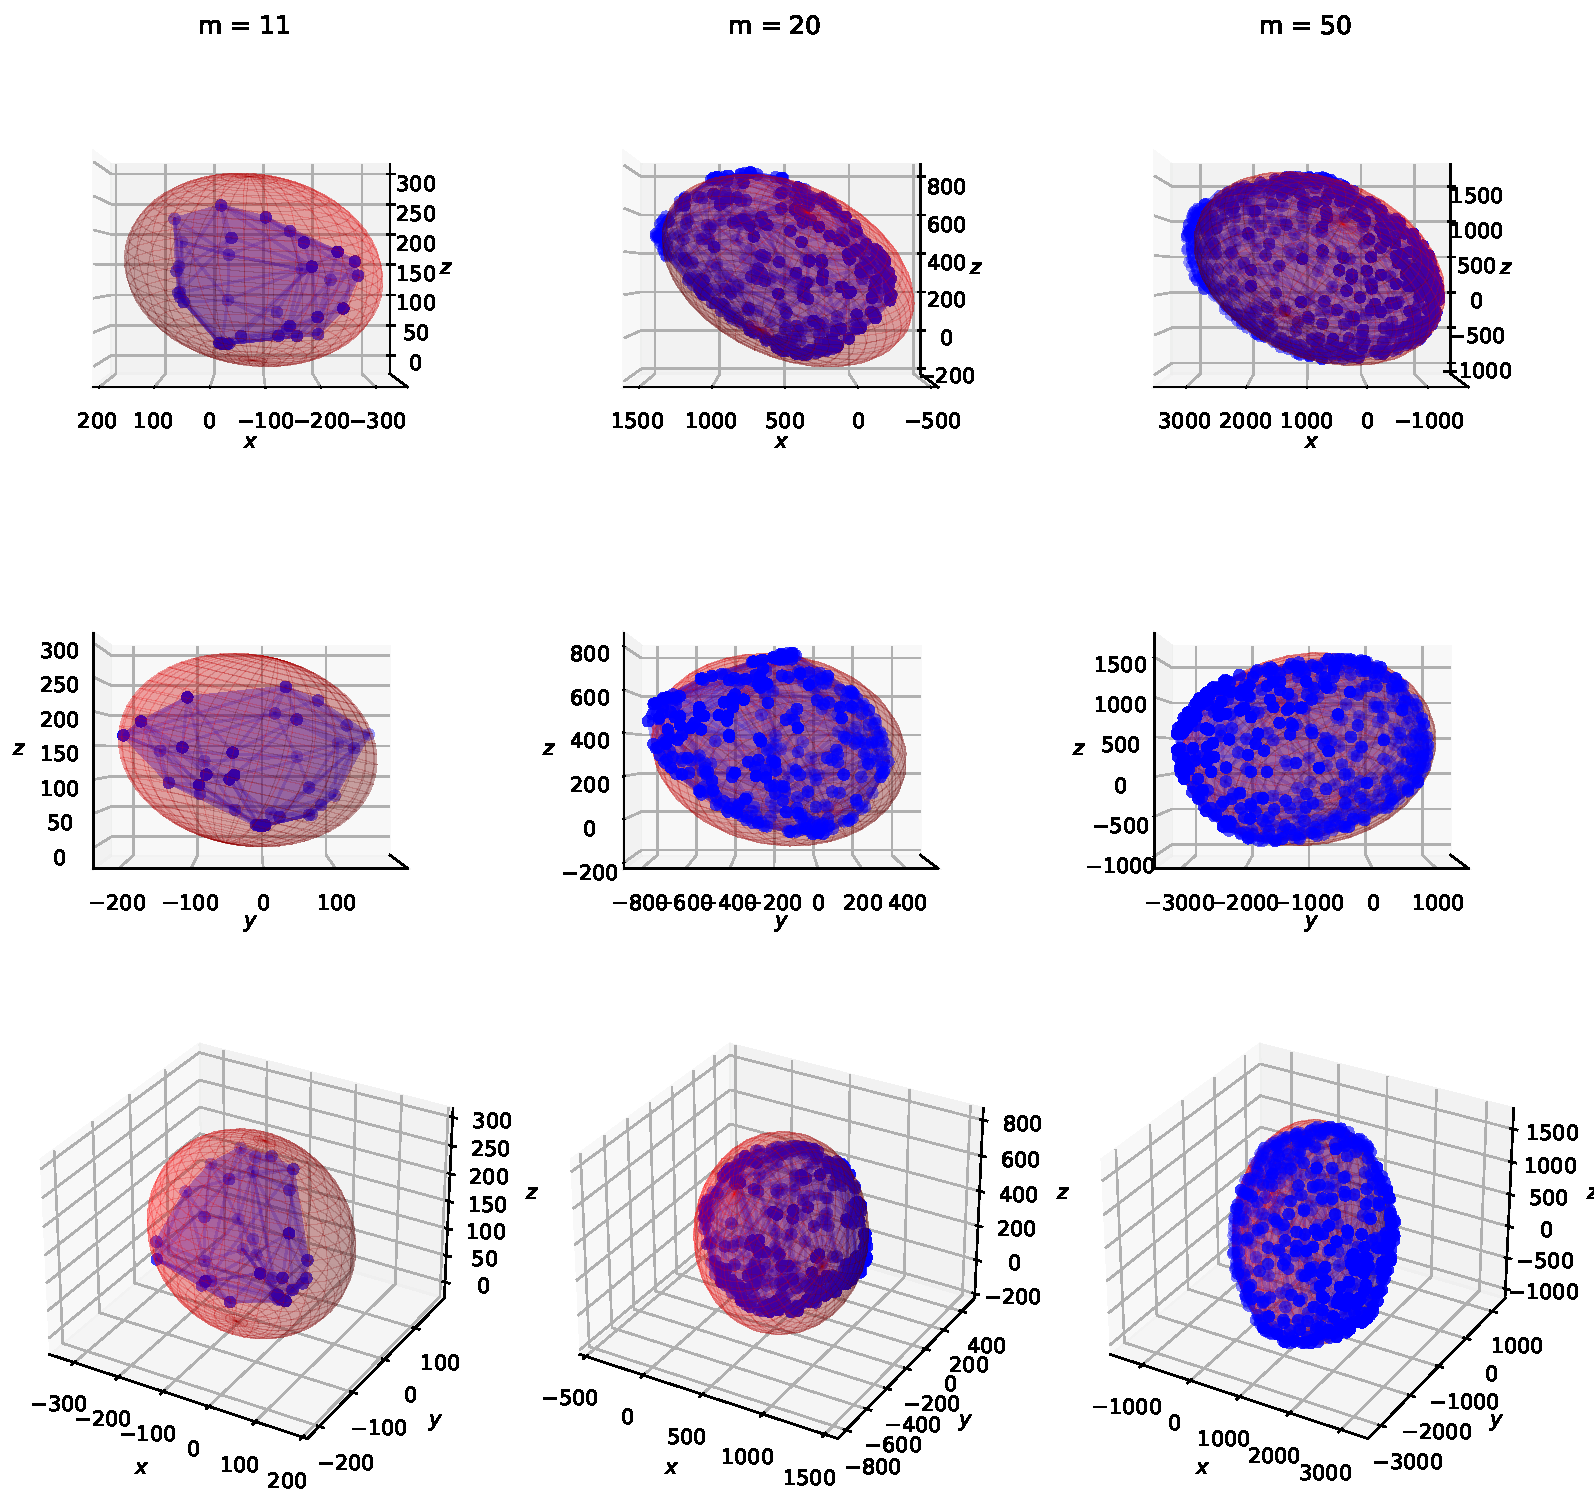
\includegraphics[trim={0 700 0 0},clip, width=0.9\linewidth]{img/chapter_3/myIma5_projection_constant.pdf}
    \end{minipage}
    \begin{minipage}{1\linewidth}
        \centering
        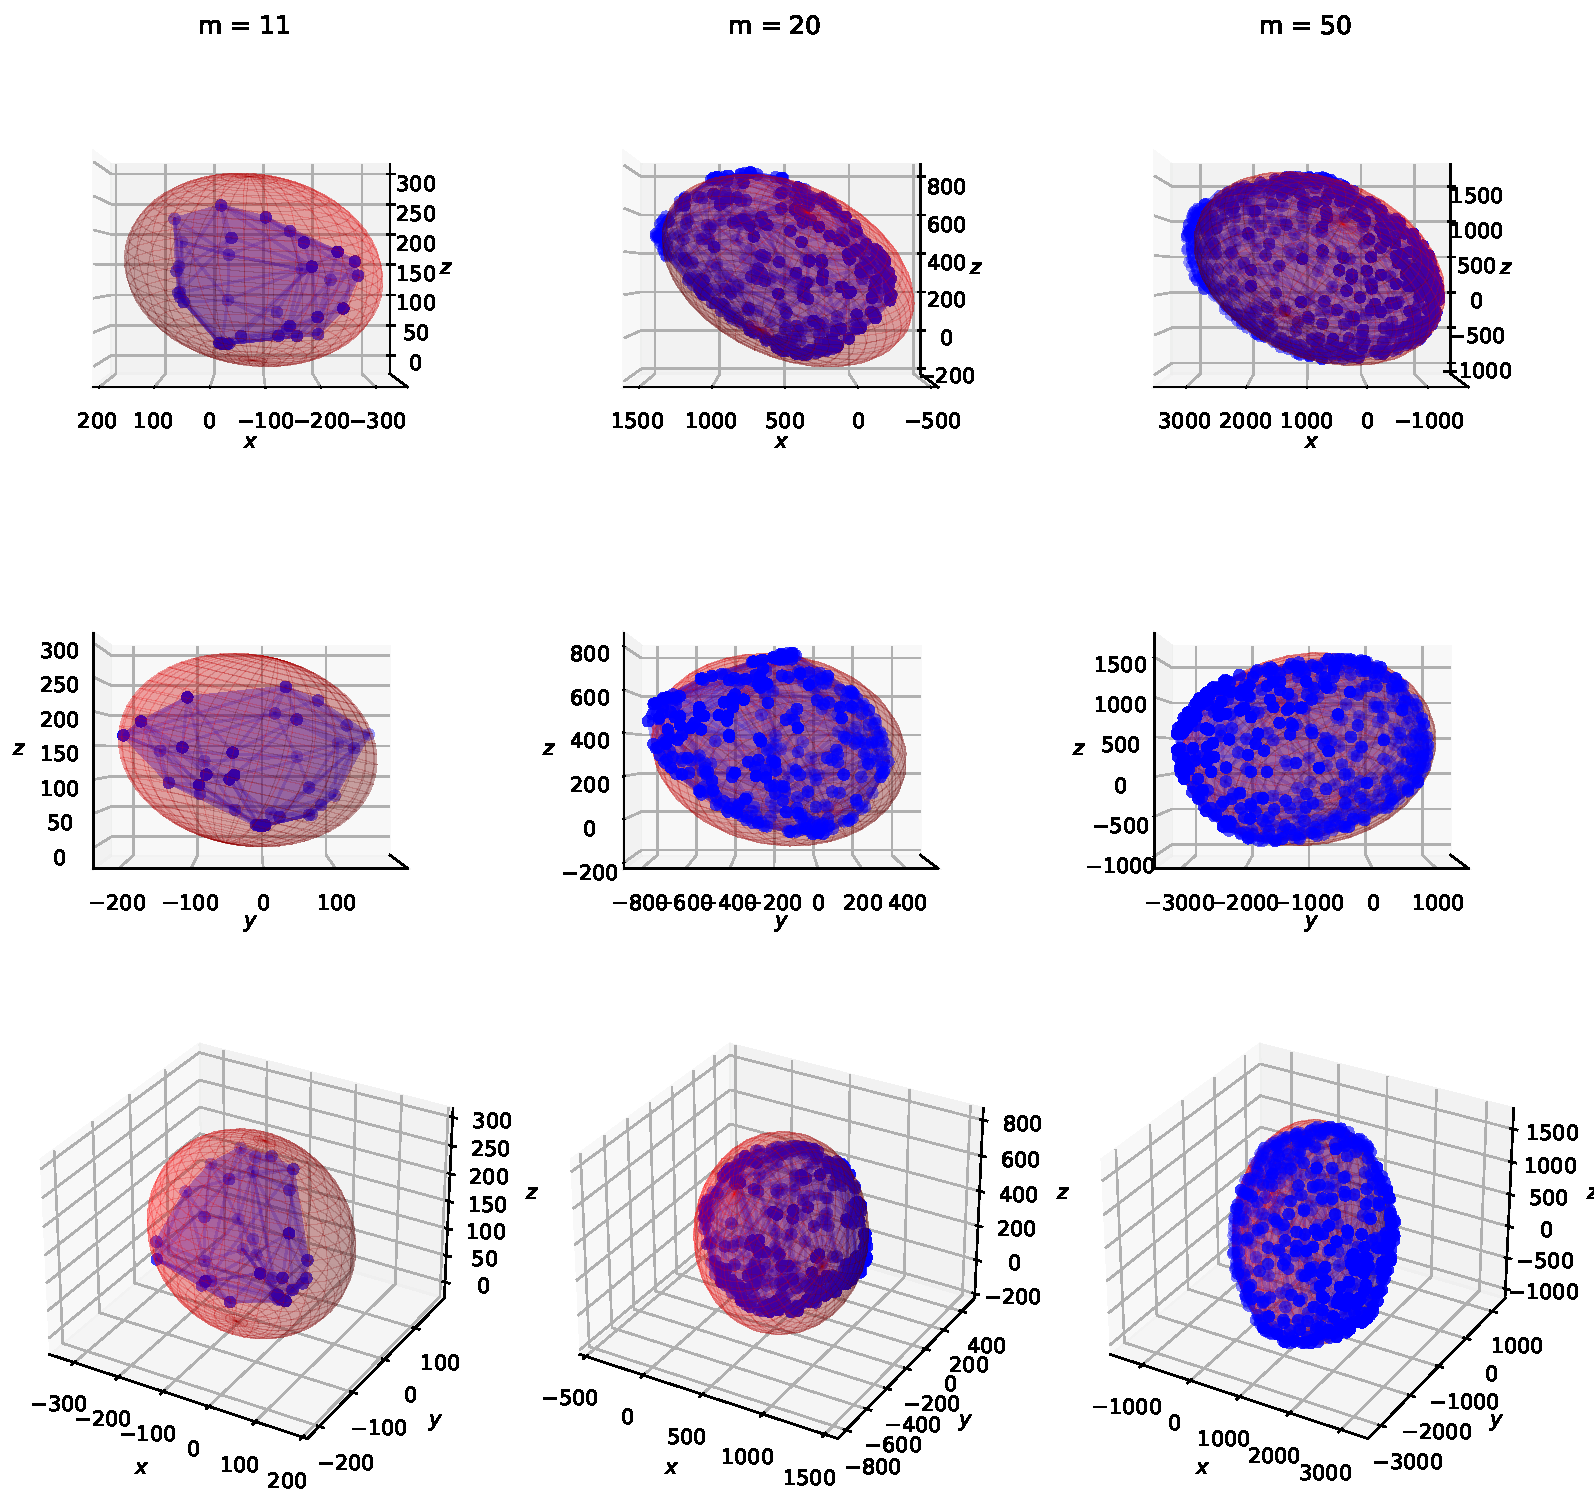
\includegraphics[trim={0 500 0 60},clip, width=0.9\linewidth]{img/chapter_3/myIma5_projection_constant.pdf}
    \end{minipage}
    \begin{minipage}{1\linewidth}
        \centering
        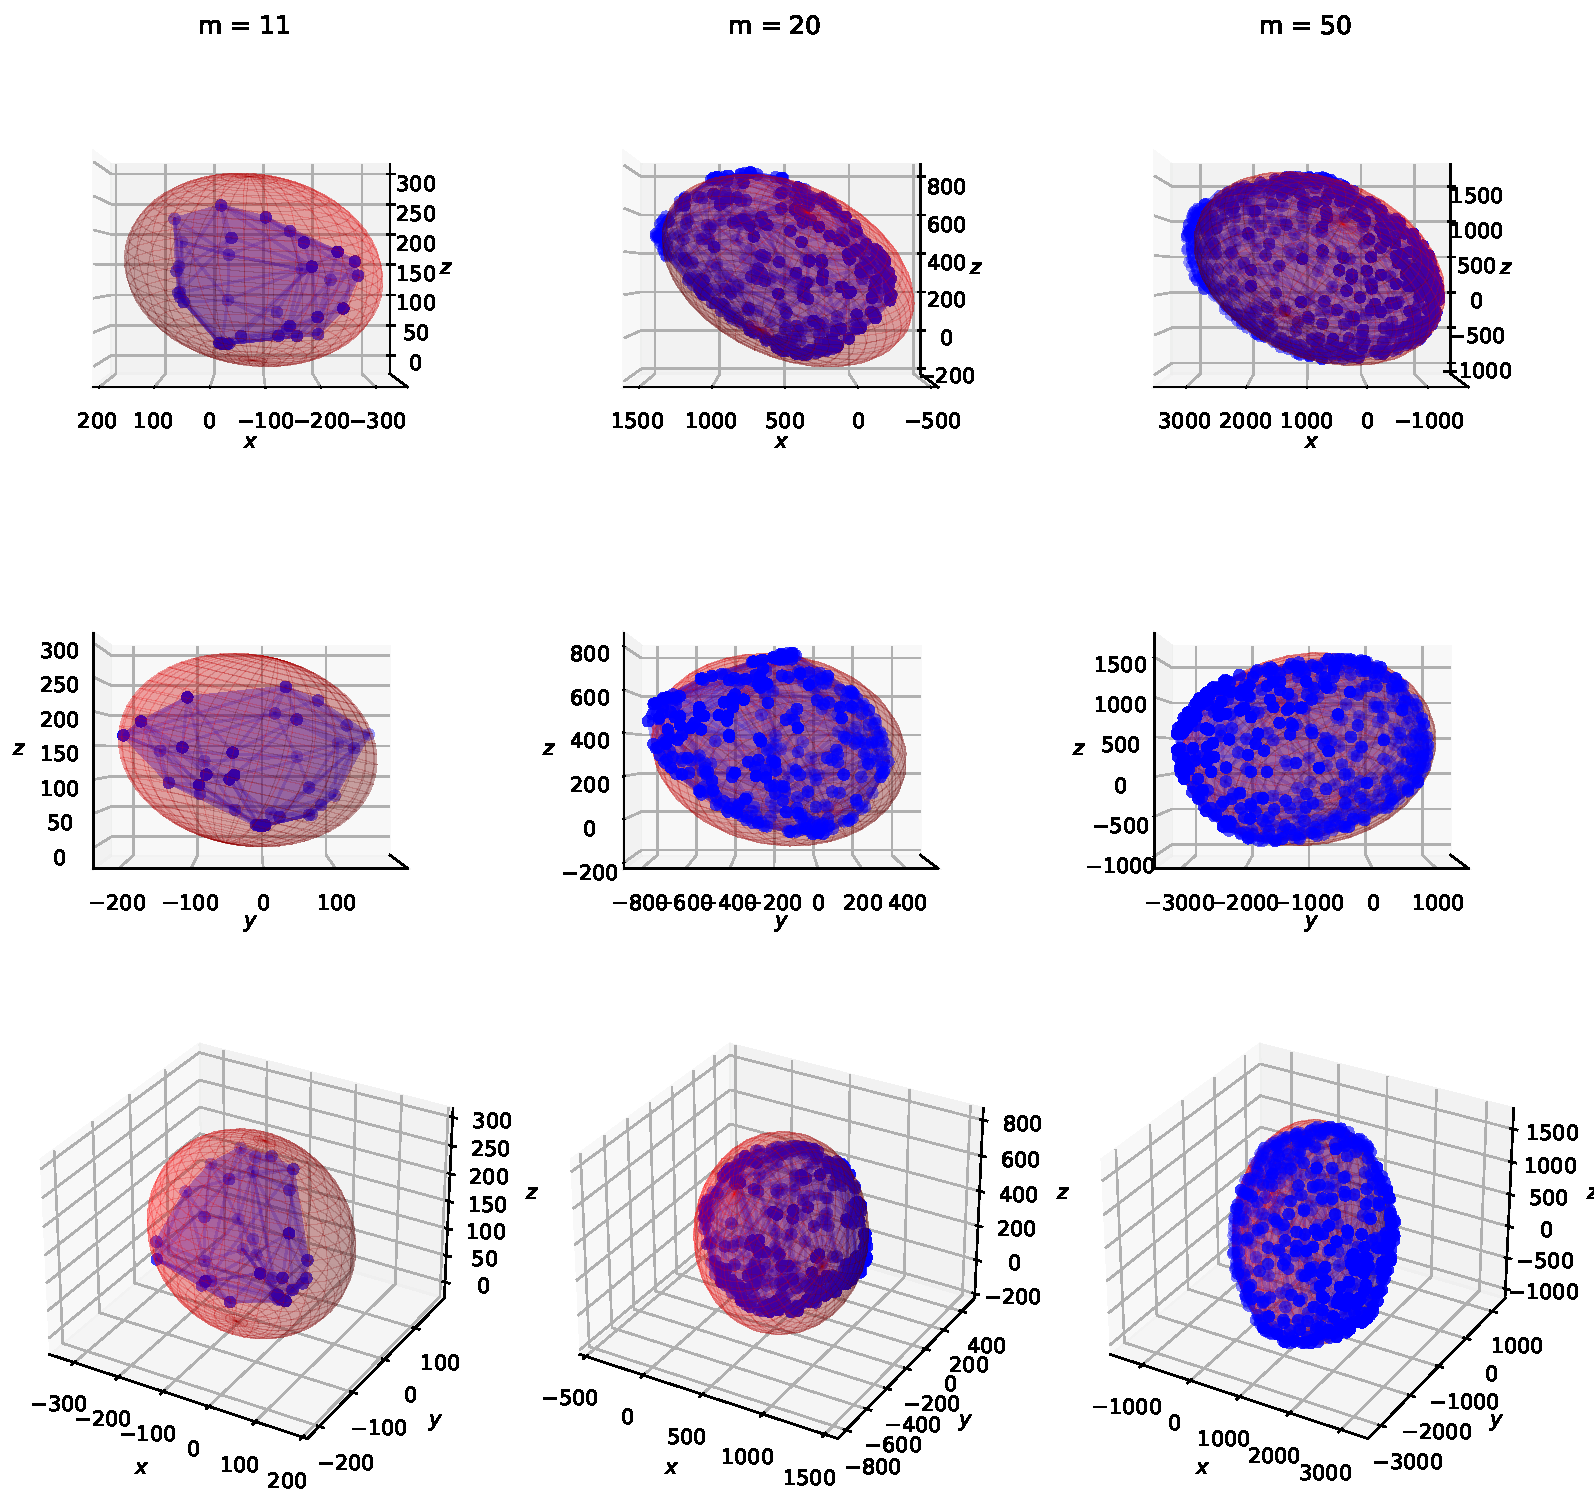
\includegraphics[trim={0 255 0 300},clip, width=0.9\linewidth]{img/chapter_3/myIma5_projection_constant.pdf}
    \end{minipage}
    \begin{minipage}{1\linewidth}
        \centering
        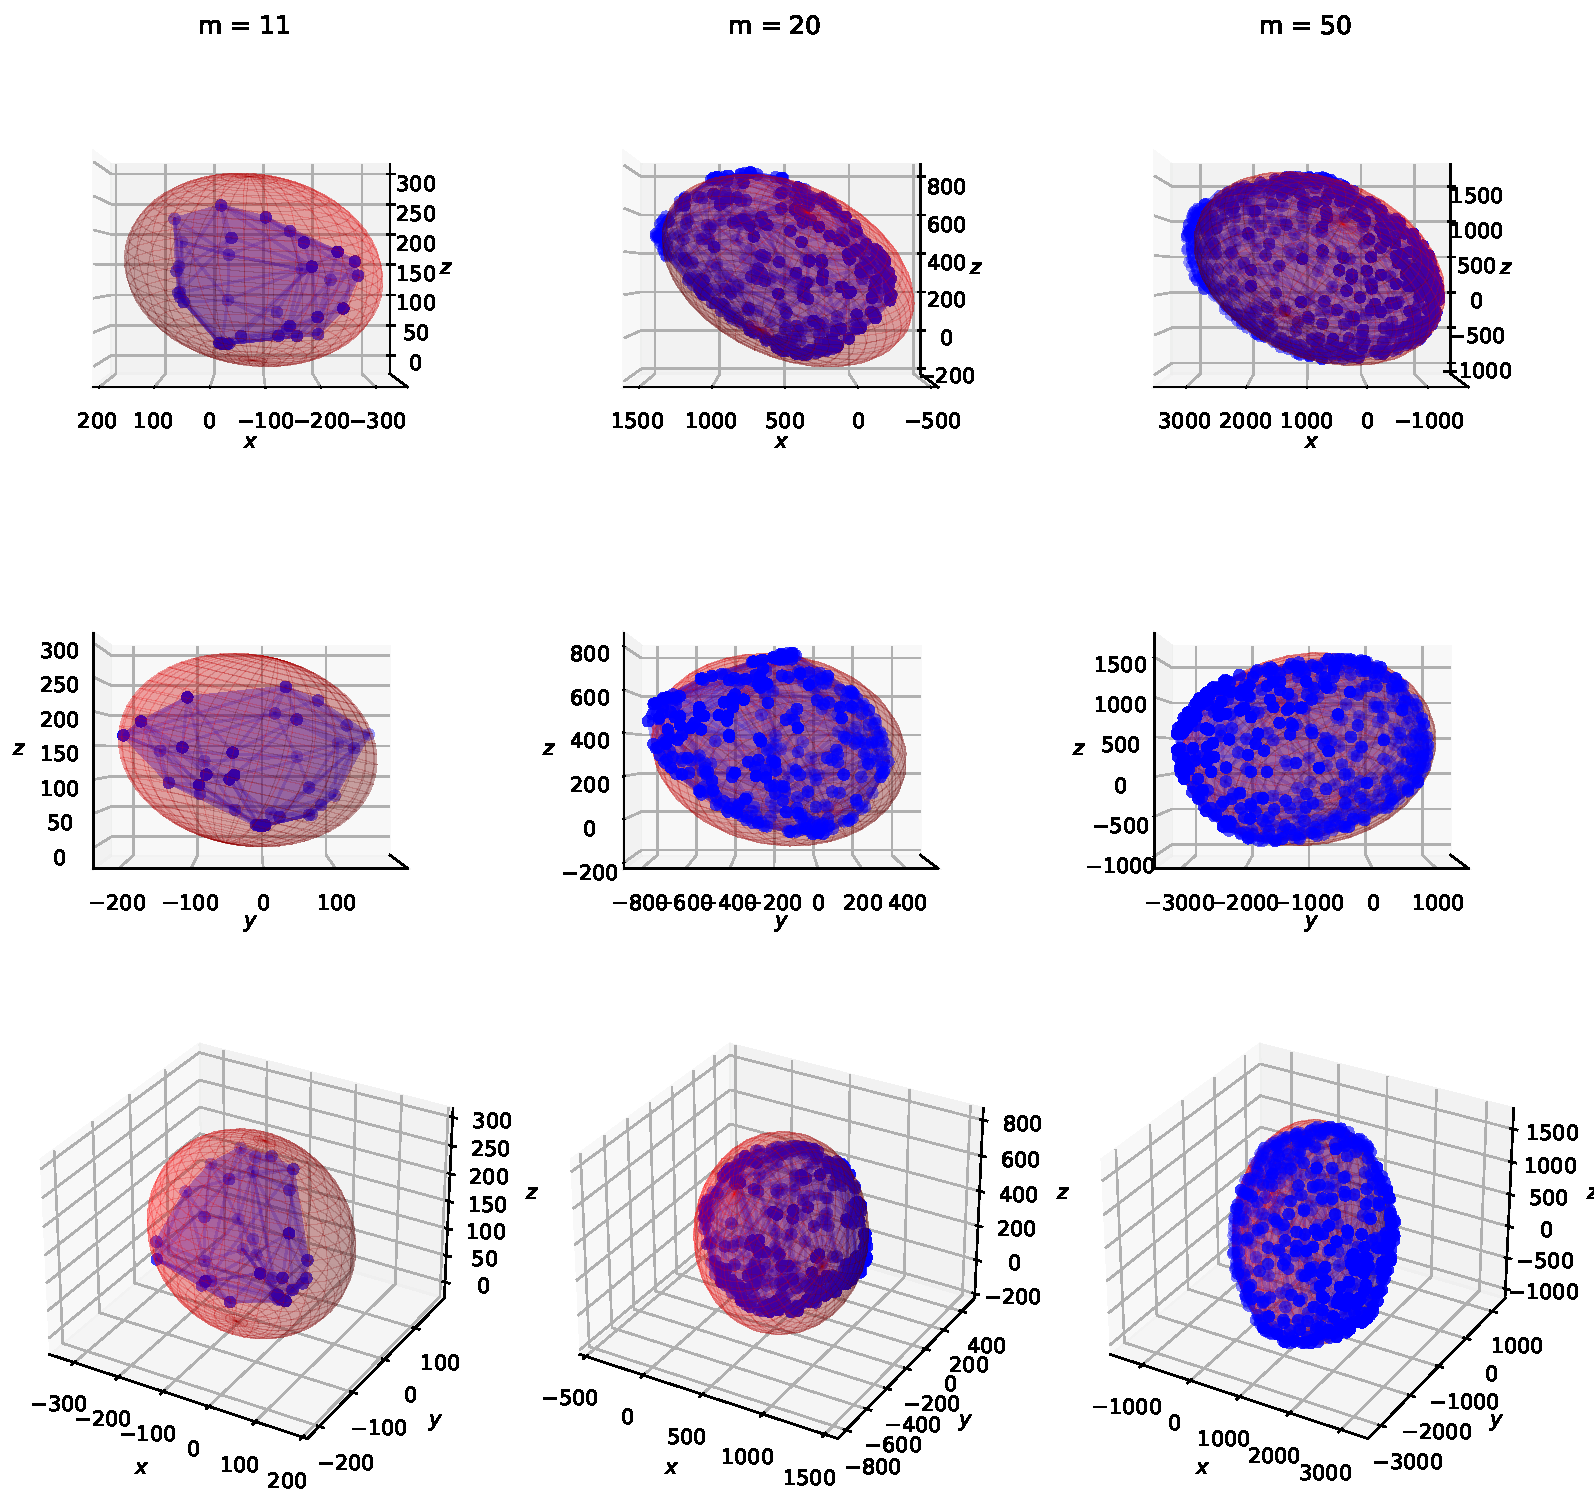
\includegraphics[trim={0 0 0 500},clip, width=0.9\linewidth]{img/chapter_3/myIma5_projection_constant.pdf}
    \end{minipage}
    
    
    \caption{Each column correspond to a different number of muscles ($m=11$, $20$ and $50$). The force polytopes (in blue) are generated by a random projection of a $m$-cube of edge length $1000$ over a $7$-dimensional torque space and intersected with a random $3$D space. As the number of muscles increases, the computed ellipsoidal approximation (in red) gets qualitatively better, and accounts for the dimension of the tension set $m$. This is due to the projection constant which is, by definition, described for $m$ sufficiently large.
    }
    \label{fig:example_proj_constant_applied}
\end{figure}


\section{Evaluating the torque contribution of muscle paths}
\label{sec:sensitivity}

This section is a surprising application of the previous theoretical knowledge gathered in this chapter in order to quantify how much does the geometry of muscles (or muscle paths description) itself impacts the force feasible set. The previous sections showed that a large amount of muscle characterizes its ellipsoidal shape, and we have computable values to return such an ellipsoid approximation.

The geometry of a muscle is dependent for each subject. When scaling a generic musculoskeletal model, a classic starting point is to scale bone lengths. If a muscle path is described as successive segments, then each point on the path should also be adapted to the subject. Since our context is not in vivo, we question the necessity of adapting the path points. In simple words, we want to quantify how does muscle geometry influences the force feasible set.

We shall consider a practical approach using Holzbaur's upper limb musculoskeletal model \cite{holzbaurModelUpperExtremity2005}. It has $7$ degrees-of-freedom to describe the shoulder motion, the elbow joint and the wrist. It is equipped with $50$ muscles, each of them containing $2$ to $12$ path points in OpenSim. Each point has an initial position value located in a body of reference.

Our approach is straight-forward. Consider a certain amount of joint configurations. For each of them, each path point location of each muscle is sampled from a uniform distribution of length $0.005$ meters from the default location. This is equivalent to consider a cube of edge length $0.01$ centers at the default location and uniformly draw samples in this cube. 

Now, we argued that since there are a lot of muscles, the tension set can be modelized as a transformation of the unit sphere (\emph{i.e.} an ellipsoid). For any joint configuration, let's assume it is a unit sphere in $\mathbb{R}^{50}$. Its radius is normalized since we are interested in how the tension set metric transforms \emph{at worst} according to muscle geometry. To describe the metric of the force feasible set, we shall use its reformulation as an \emph{intersection-then-projection}, as seen in section \ref{sec:ellipsoidal_shape_ffs}. In this case, its ball is described as the tension set sphere intersected with the space $K$, so it is an ellipsoid, then it is projected via the lever arm matrix onto $\im J^T$. Computing the metric deformation in the worst case is the purpose of the operator norm, and in our context we are considering a deformation from a sphere to an ellipsoid, so the computation is described in the $2$-norm of the generators of the resulting ellipsoid.

The following table describes the $2$-norm computation for $4$ considered postures $100$ random variations of each points describing Holzbaur's muscle geometry. The postures are defined as 
\begin{itemize}[noitemsep]
    \item {$\mathbf{q}_1 = (13,12.5,-41,30.5,-5.3,0.19,-0.76)$}
    \item {$\mathbf{q}_2 = (13,90,-41,30.5,-5.3,0.19,-0.76)$}
    \item {$\mathbf{q}_3 = (37,90,21,30.5,-5,0.19,-0.76)$}
    \item {$\mathbf{q}_4 = (37,31,21,30.5,-1.3,0.19,-0.76)$}
    \item {$\mathbf{q}_5 = (37,31,21,76,42,0.19,-0.76)$}
    \item {$\mathbf{q}_6 = (110,31,21,76,42,0.19,-0.76)$}
    \item {$\mathbf{q}_7 = (110,10,21,76,74,0.19,-0.76)$}
    \item {$\mathbf{q}_8 = (96,79,120,76,74,0.19,-0.76)$}
\end{itemize}

\begin{table}[!ht]
    \centering
    \begin{tabular}{|c||c|c|}
    \hline
    Posture & \makecell{Mean of $2$-norm} & Standard deviation of $2$-norm \\
    \hline
    \hline
    $\mathbf{q}_1$ & $0.1140$ & $0.0021$ \\ \hline
    $\mathbf{q}_2$ & $0.0822$ & $0.0055$ \\ \hline
    $\mathbf{q}_3$ & $0.0953$ & $0.0012$ \\ \hline
    $\mathbf{q}_4$ & $0.0843$ & $0.0017$ \\ \hline
    $\mathbf{q}_5$ & $0.0929$ & $0.0012$ \\ \hline
    $\mathbf{q}_6$ & $0.0749$ & $0.0028$ \\ \hline
    $\mathbf{q}_7$ & $0.0859$ & $0.0019$ \\ \hline
    $\mathbf{q}_8$ & $0.0980$ & $0.0018$ \\ \hline
    \end{tabular}
    \caption{Mean and standard deviation of the $2$-norm of the force feasible set computed as an intersection then projection of the tension ellipsoid. $100$ random variations of the initial coordinates of each point of each muscles in Holzbaur's upper limb musculoskeletal model.}
    \label{tab:sensitivity}
\end{table}

The important result is the standard deviation: the closer to $0$ it is, the less impact the muscle geometry has on the deformation of the tension set. Note that this is a set-theoretic interpretation, it is not applicable in a more vectorized point of view. What matters is not how a specific muscle tension combination is deformed, but how \emph{everything} deforms \emph{as a whole}.

Almost all standard deviations are close to zero, but remember that we work with a unit sphere transformation, so the order of magnitude is necessarily less than $1$. Such low means are simply reflecting the projected volume problem: we transform a sphere in $50$ dimensions, which has a low volume even if its vectors are of norm $1$. As a result, the force feasible ellipsoid does have this low volume reflected in its small vectors. This implies that we must be extremely careful with the order of magnitude of everything displayed in this table.

For instance, consider the first posture $\mathbf{q}_1$. The mean indicates that in average, for all muscle path points considered, a combination of muscle tensions amounting to a total of $1$N is in the worst possible case roughly equivalent to $0.1140$Nm. In more trivial terms, in the average case the tension exerted by some muscles can maximally account for about $11$\% of $1$Nm.

Consider that each muscle can maximally exert a tension of $1000$N, but any combination of muscles too. For all muscle geometry variations, the above-mentionned standard deviation represents the worst case deformation size of a vector in the tension set when it is transformed as the force feasible set (expressed in the torque space). This means that our muscles exerting together $1000$N produces a torque size between $1000\times (0.1140 - 0.0021) = 111.9$Nm and $1000\times (0.1140 + 0.0021) = 116.1$Nm. In context, this means that if it was possible to personalize precisely the muscle geometry of a subject, the produced force feasible set expressed in the torque space would have, \underline{at worst}, a size difference of $116.1-111.9=4.2$Nm  in posture $\mathbf{q}_1$.

Let's summarize these worst-case scenarii in the following table:

\begin{table}[!ht]
    \centering
    \begin{tabular}{|c||c|c|}
    \hline
    Posture & \makecell{Worst size difference \\ using max-min} & \makecell{Maximal torque contribution difference \\ between two geometries if \\ all muscles have a tension of $1000$N} \\
    \hline
    \hline
    $\mathbf{q}_1$ & $0.0099$ & $9.9$ Nm \\ \hline
    $\mathbf{q}_2$ & $0.0554$ & $55.4$ Nm \\ \hline
    $\mathbf{q}_3$ & $0.0066$ & $6.6$ Nm \\ \hline
    $\mathbf{q}_4$ & $0.0091$ & $9.1$ Nm \\ \hline
    $\mathbf{q}_5$ & $0.0055$ & $5.5$ Nm \\ \hline
    $\mathbf{q}_6$ & $0.0131$ & $13.1$ Nm \\ \hline
    $\mathbf{q}_7$ & $0.0084$ & $8.4$ Nm \\ \hline
    $\mathbf{q}_8$ & $0.0098$ & $9.8$ Nm \\ \hline
    \end{tabular}
    \caption{Worst metric size difference of any muscle tension vector projected onto the force feasible set expressed in the torque space when considering variations of muscle geometry. Each value is computed using the range.}
    \label{tab:sensitivity2}
\end{table}

All these results are meaningful in the sense that they explain how two ``close'' muscle geometries impact the possible torque produced according to the posture.

In our context, this means that if a tension set is assumed to be spherical, we can for specific postures only, use Holzbaur's default muscle path points knowingly \emph{how much we can derive from a better personalized musculoskeletal model}.

Quantifying the error in our assumptions is crucial, and we propose an index measuring specifically the contribution of the muscle geometry to produce a force feasible set (expressed in the torque space).

Also, to conclude this section, we hypothesize that considering a much larger number of muscles should lead to lesser difference in between two close muscle geometries. The intuition behind this is as follows: the more muscles are considered, the more probability the force feasible set has to be ellipsoidal. But this applies as well for the torque feasible set. This is the geometric perspective, but the metric point of view is more adequate to state equivalently that the more muscles are considered, the less impact has a single muscle on the torque space. Naturally, the difference of total impact between various muscle geometries is less and less.
We even assume that for an infinite number of muscles, the projection between the tension space and the torque space is less and less dependent on the muscle geometry, even not dependent. 
It does not mean that the geometric muscle components are not inside the force feasible set formulation, but that there exists a global projection transforming the tension set directly to the force feasible set without requiring to pass by the torque space.

We actually do have some indications on this perfect projection: by rewritting the force feasible set as an intersection-then-section, we showed that the tension set (in $\IRm$) is first intersected by a space $K$ of dimension $m-(n-p)$. When the number of muscles is large, this is similar to not intersect anything at all. The projection thereafter depends on the geometry of muscles. If we assume that any geometry projects similarly through a matrix $P\in \IRnm$ (\emph{i.e.} muscle tensions have the same degree of impact on the force feasible set metric for anyone), then the direct link between the tension space and the force space would be $(J^T)^+P(\mathcal{T})$. In other words, only the mean muscle tension and the arm geometry and motion matters.

Chapter 5 will make this assumption in order to predict force feasible sets in an individual.

\usection{Conclusion}
\label{sec:approx_discussion}

The underlying objective of this chapter was to deeply understand the relations between all elements in the force feasible set general model $\mathcal{F}$ described initially as
$$\mathcal{F} = \left\{ \mathbf{f}\in \IRp \mid J^T\mathbf{f} = -L^T\mathbf{t} - \mathbf{G},\quad \mathbf{t}\in \mathcal{T} \right\}$$

In a more abstract manner, this is equivalent to assume a surjective affine map $\psi\,\colon \IRm\rightarrow \IRn$ and an injective map $\phi\,\colon \IRp\rightarrow \IRn$ such that 
$$\mathcal{F} = \im \phi \cap \psi(\mathcal{T})$$

While this geometric point of view can help us understand the operations involved in this description, the physics behind it should be also considered: the unit measure used to describe elements of $\mathcal{F}$ is the deformation of the unit measure of the tension set $\mathcal{T}$. The link between geometry and metric is already a mathematical field of study, called the Banach space theory. By studying a more precise subbranch of it, the Local Theory, we showed by rewritting $\mathcal{F}$ that whatever the choice of $\mathcal{T}$, $\mathcal{F}$ must resembles an ellipsoid in shape. Working with an ellipsoid is advantageous, in that it allows easier computational tools to describe a set.

However, computing explicitely this ellipsoid is not straight-forward. We noticed a relationship between volumes of sphere projections and cube projections: they are related by the dimension of the tension set (\emph{i.e.} the number of muscles considered). This relation $\lambda$, called \emph{projection constant}, is explicitely computable and corresponds to how much should be the radius of a sphere to behave as if it were a cube in dimension $m$. In a more metric sense, it expresses how the Newton unit in the tension set is approximately seen as $\frac{1}{\lambda}$ of a Newton-meter unit.

This metric perspective allows us, in a context with a large number of muscles compared to the torque space dimension, to directly quantify how the muscle geometry has an impact on the force feasible set using the operator norm of $-L^T$. As an application, it is thus possible to consider small variations of all muscle paths and compute how this norm varies for a given posture. If the range of these norms is less than a context-dependant value of choice, it can be decided if whether or not the personalization of the muscle geometry to an individual should be of concern when studying produced force and torque feasible sets in isometric condition. 

To summarize: 
\begin{enumerate}
    \item {\textbf{Section \ref{sec:ellipsoidal_shape_ffs}:} the force and torque feasible sets are likely to have an ellipsoidal shape when considering a large number of muscles;}
    \item {\textbf{Section \ref{sec:projected_volume_problem}:} an ellipsoid approximation can be computed knowing the number of muscles and how much tension interactions are to be considered;}
    \item {\textbf{Section \ref{sec:sensitivity}:} the force feasible set depends on the posture, the geometry of muscles, their tensions and their interactions. The contribution of these components has been understood as such: 1) interactions describe the force feasible set global shape, 2) its global orientation is mainly described by the arm posture, and 3) tensions values as well as the muscle geometry and the number of muscles describe its global size.  In order to separate the muscle geometry impact from the tensions and number of muscles, we can study it through a specific index related directly to the computation of the operator $2$-norm of $-L^T$. This computation has a meaning only if the number of muscles is large so that an ellipsoid approximation of the force feasible set makes sense.}
\end{enumerate}

While this theoretic results help us to understand the force feasible set modelization, there remains to apply them. The next chapter \ref{chapter:4} is dedicated to in silico applications, in order to measure how an ellipsoidal approximation can help us in predicting force capacities. This chapter will also consider more practical tools to reconstruct a musculoskeletal model when a \emph{low} number of muscles are considered. This will lead to chapter \ref{chapter:5} in which we will add new assumptions on the neuromuscular behavior in order to reconstruct a musculoskeletal model based on experimental data.
